\pagestyle{empty}
\graphicspath{{Fundamentos/}}
\part{Los fundamentos}\label{Fundamentos}

\sffamily

\vspace*{4cm}

En esta parte comenzar�s a conocer qu� es un SIG, el porqu� de su existencia, su utilidad, y los distintos componentes en que podemos dividirlos, y que ser�n estudiados de forma separada a lo largo de todo el libro. Adem�s de esto, se presentan en esta parte algunos conceptos relativos a ciencias afines como la cartograf�a o la geodesia, que son imprescindibles para poder comprender en profundidad los SIG y sus distintas facetas.

\begin{itemize}

\item El cap�tulo \ref{Introduccion_fundamentos} presenta el entorno de los SIG, mostrando al lector el contenido gen�rico sobre el que trata no solo esta parte, sino el libro al completo. Se describen las ideas fundamentales sobre SIG y los elementos que lo forman.

\item El cap�tulo \ref{Historia} recorre la breve pero intensa historia de los SIG, desde su origen hasta nuestros d�as.

\item En el cap�tulo \ref{Fundamentos_cartograficos} se resumen los conceptos cartogr�ficos y geod�sicos b�sicos, imprescindibles para el d�a a d�a del trabajo con un SIG.

\end{itemize}

\rmfamily
%\twocolumn

\chapter{Introducci�n. �Qu� es un SIG?}\label{Introduccion_fundamentos}
\pagestyle{fancy}

\begin{keypoints}
�Qu� es un Sistema de Informaci�n Geogr�fica (SIG)? $\bullet$ �Para qu� sirve? $\bullet$ �C�mo se trabaja con un SIG?  $\bullet$ �Qu� elementos fundamentales comprende? $\bullet$ �Qu� es la Ciencia de la Informaci�n Geogr�fica?  $\bullet$ �En qu� otras disciplinas se fundamenta?
\end{keypoints}

\bigskip

\begin{intro}
Este cap�tulo presenta los conceptos fundamentales sobre Sistemas de Informaci�n Geogr�fica (SIG), definiendo estos y presentando tanto sus capacidades fundamentales como la forma en que estas pueden ser aprovechadas. Asimismo, se presentan los SIG como sistemas complejos, y se describe cada uno de sus componentes principales. El cap�tulo presenta una visi�n global del �mbito de los SIG y de la ciencia asociada a los SIG como disciplina independiente, al tiempo que muestra el contexto en el que el desarrollo y utilizaci�n de estos se produce en la actualidad.
\end{intro}

\section{Introducci�n}

Para justificar la importancia de los Sistemas de Informaci�n Geogr�fica (SIG) y el papel que estos juegan hoy en d�a, es habitual en libros como este citar el hecho de que aproximadamente un 70\% de la informaci�n que manejamos en cualquier tipo de disciplina est� georreferenciada. Es decir, que se trata de informaci�n a la cual puede asignarse una posici�n geogr�fica, y es por tanto informaci�n que viene acompa�ada de otra informaci�n adicional relativa a su localizaci�n. 

Si bien es probable que este porcentaje no haya variado desde que comenz� a mencionarse en los libros sobre SIG, la situaci�n es en la actualidad m�s favorable que nunca para el desarrollo de herramientas que permitan la utilizaci�n de toda esa informaci�n al tiempo que se consideran los datos relativos a su posici�n en el espacio. Esto es as� no solo porque trabajamos con gran cantidad de informaci�n referenciada geogr�ficamente, sino porque somos cada d�a m�s conscientes de la importancia que esa componente geogr�fica tiene. La geograf�a ha pasado de ser un �mbito particular con cierta relaci�n con otros campos a ser un elemento fundamental incorporado a la mayor parte de las disciplinas. Y no solo en el terreno cient�fico, sino en el terreno mismo de la vida diaria, donde toda esta informaci�n desempe�a un papel de gran importancia.

La utilizaci�n de cartograf�a ha dado un vuelco radical en el plazo de unas d�cadas, permitiendo nuevas posibilidades y acercando la informaci�n cartogr�fica como herramienta de primer orden a un p�blico amplio y diverso. La elaboraci�n misma de cartograf�a ha pasado de ser terreno exclusivo de profesionales del sector a ser una labor abierta donde las nuevas tecnolog�as, especialmente las de corte colaborativo, han permitido que otro tipo de usuarios desarrollen y compartan informaci�n cartogr�fica.

En este sentido, los SIG no son solo herramientas dentro de ese contexto de gran importancia de la informaci�n geogr�fica, sino en gran medida responsables de que esa situaci�n sea tal, pues su contribuci�n dentro del panorama relativo a la geograf�a ha sido vital para impulsar esta y hacerla llegar hasta su lugar actual. En una sociedad donde la informaci�n y la tecnolog�a son dos de los pilares fundamentales, los SIG son, sin lugar a dudas, la tecnolog�a estandarte para el manejo de informaci�n geogr�fica, y los elementos b�sicos que canalizan la gesti�n de todo aquello que, de un modo u otro, presente una componente geogr�fica susceptible de ser aprovechada.

As�, un SIG es fundamentalmente una herramienta para trabajar con informaci�n georreferenciada, una definici�n en la que pueden entrar un gran n�mero de tecnolog�as y de otros elementos no tecnol�gicos, los cuales veremos a lo largo de este libro.


\section{Un peque�o ejemplo}

Para comenzar a tener una idea correcta de lo que representa e implica un SIG, veamos un sencillo ejemplo. Supongamos el caso de un organismo o empresa cuyo trabajo incluye la gesti�n de una masa forestal. Este trabajo de gesti�n implicar� algunas actividades como las siguientes, en las cuales se utiliza en mayor o menor medida informaci�n georreferenciada.

\begin{itemize}
	\item Delimitaci�n de las distintas zonas inventariables y unidades dasocr�ticas (montes, cantones, rodales, etc.)
	\item Dise�o de inventarios
	\item Realizaci�n de inventarios y gesti�n de sus datos para la obtenci�n de resultados tales como estimaciones de vol�menes maderables.
	\item Gesti�n de infraestructuras del monte tales como v�as de comunicaci�n, torres de vigilancia contra incendios, etc.
\end{itemize}

En un contexto en el que no existen medios inform�ticos para la realizaci�n de estas tareas, gran parte de ellas se desarrollar�n con el apoyo de cartograf�a cl�sica. As�, las zonas inventariables se delimitar�n sobre un plano, y sobre este mismo pueden medirse sus superficies con la ayuda de un plan�metro. En ese mismo plano se localizan las parcelas a muestrear en un inventario, y los operarios encargados de llegar hasta esas parcelas y realizar las mediciones pertinentes se ayudan de �l para localizarlas y desplazarse sobre el terreno.

Los resultados del inventario se almacenan en estadillos, y las operaciones correspondientes al an�lisis estad�stico de estos se realizan de forma manual, as� como la comparaci�n con inventarios anteriores que permiten estudiar la evoluci�n del monte.

La presencia de medios inform�ticos facilita estas tareas, mejorando por una parte la gesti�n de los datos, y por otra las operaciones que pueden realizarse sobre estos. Una sencilla hoja de c�lculo, por ejemplo, es una herramienta imprescindible para la gesti�n de los datos de un inventario, haciendo que todo el trabajo con ellos resulte m�s eficiente y adecuado.

En lo relativo a la cartograf�a, la situaci�n, aunque con un desarrollo (y especialmente una implantaci�n de usuarios) m�s reciente, no es muy distinta. Ventajas similares a las que aporta una hoja de c�lculo pueden encontrarse en una aplicaci�n que permitiera utilizar mapas y planos \emph{dentro} de un ordenador, con la consecuente ganancia en productividad, eficiencia y precisi�n. Esta aplicaci�n destinada al manejo de cartograf�a es el concepto b�sico de un Sistema de Informaci�n Geogr�fica, y la idea fundamental a partir de la cual comenz� el desarrollo de estos.

Con un SIG, la cartograf�a de esa masa forestal puede visualizarse y almacenarse en un ordenador personal, y pueden realizarse sin dificultad y de forma instant�nea c�lculos tales como mediciones de cada una de las entidades. La creaci�n de nueva informaci�n cartogr�fica se lleva a cabo ya en el propio SIG, del mismo modo que la edici�n de cartograf�a ya existente. Modificar el l�mite de una unidad dasocr�tica o el trazado de una v�a, o crear la cartograf�a correspondiente a las parcelas de inventario son tareas que, en nuestro caso de ejemplo, se realizan hoy en d�a empleando un SIG.

Las ventajas que esto tiene son muchas, especialmente las relacionadas con una mejor gesti�n del conjunto de distintos datos que se manejan, as� como las relativas a la sencillez con que pueden modificarse estos datos\footnote{Veremos con m�s detalle las ventajas de los datos digitales frente a los datos anal�gicos en el cap�tulo \ref{Fuentes_datos}}.

Otras de las labores donde un SIG demuestra su utilidad es en el an�lisis. Los datos geogr�ficos pueden ser objeto de gran n�mero de distintos an�lisis, y la capacidad de c�mputo de un ordenador es necesaria para muchos de ellos. La herramienta id�nea para implementar esos algoritmos y operaciones de an�lisis espacial es el SIG, pues ya contiene los elementos necesarios para el manejo de los datos de partida, es decir, aquellos que contienen la informaci�n georreferenciada.

Y, por supuesto, un SIG conectado a un perif�rico de impresi�n permite generar una versi�n anal�gica a partir de la informaci�n con la que se trabaja, teniendo la capacidad de crear cartograf�a en papel cuando as� se requiera.

En otras palabras, un SIG es una herramienta que brinda a las labores de uso y manejo de informaci�n geogr�fica toda la potencia de un ordenador, pues ha sido dise�ada espec�ficamente para trabajar con este tipo particular de informaci�n.

No obstante, m�s all� de todas estas tareas antes mencionadas el concepto de SIG ha evolucionado hasta convertir actualmente a estos en sistemas complejos que buscan dar soluci�n a todas las necesidades que se presentan en situaciones similares a la del ejemplo comentado. Con la tecnolog�a actual, la incorporaci�n de elementos propios de los SIG puede llegar mucho m�s all�, y uno de los pilares m�s s�lidos de los SIG en la actualidad es su capacidad de mostrar que existe una componente espacial susceptible de ser gestionada con la ayuda de un SIG en la pr�ctica totalidad de contextos posibles.

Como sistema, un SIG puede gestionar la cartograf�a necesaria para la gesti�n integral del monte, y hacerlo adem�s de forma centralizada. De este modo, se garantiza el rigor y la robustez de los datos base, ya que el SIG es el encargado de canalizar la utilizaci�n de estos por parte de todos los usuarios. Esto es de especial importancia en caso de que se editen los datos, ya que esta edici�n tambi�n est� centralizada, y un usuario ve reflejarse en su cartograf�a de forma inmediata los cambios realizados por otro, teniendo siempre a su disposici�n la versi�n m�s actual y, por tanto, m�s adecuada.
 
A esto puede a�adirse la utilizaci�n de SIG m�viles en dispositivos port�tiles, que permiten que el SIG se incorpore tambi�n a las fases de trabajo de campo. Esa misma cartograf�a centralizada pueden utilizarla los operarios en campo a trav�s de sus dispositivos para desarrollar su trabajo, ayud�ndose adem�s de sistemas de navegaci�n para la localizaci�n de las parcelas de un muestreo o de cualquier otro punto de inter�s al que deban desplazarse. 

Gracias a la tecnolog�a SIG, la informaci�n espacial puede ser aprovechada en mayor medida, y en muchos casos pasa de ser una informaci�n inherente a los datos pero sin una verdadera aplicaci�n, a ser un elemento sumamente enriquecedor y clave para muchos an�lisis. 

En nuestro ejemplo de gesti�n forestal, los propios datos del inventario, que antes eran fundamentalmente datos sobre las propiedades de los distintos �rboles medidos (altura, di�metro, etc.), ahora ofrecen muchas m�s posibilidades si se considera que cada uno de estos �rboles ha sido medido en una parcela dada, la cual lleva asociadas unas coordenadas concretas.

El trabajo que se desarrollaba en la hoja de c�lculo con estos datos se puede incorporar al SIG, el cual adem�s de las funciones de an�lisis estad�stico incluye funciones de an�lisis espacial. De este modo, los resultados num�ricos que se obten�an de esos an�lisis (vol�menes totales estimados, alturas medias, etc.) se ampl�an mediante resultados con mayor componente espacial, como puede ser la creaci�n de nueva cartograf�a referente a las variables principales (mapas de densidad media de arbolado, altura dominante media, etc.). 

En resumen, el SIG en su concepci�n actual es una herramienta integradora que busca abarcar en su �mbito todas las funcionalidades que se requieren para el trabajo con variables y elementos espacialmente localizados, incorporando para ello capacidades variadas que ser�n las que vayamos viendo progresivamente a lo largo de esta obra.

\section{�Qu� es un SIG?}

Partiendo del ejemplo anterior, podemos dar una definici�n m�s precisa y formal de lo que realmente es un SIG. B�sicamente, un SIG ha de permitir la realizaci�n las siguientes operaciones:

\begin{itemize}
	\item Lectura, edici�n, almacenamiento y, en t�rminos generales, gesti�n de datos espaciales.
	\item An�lisis de dichos datos. Esto puede incluir desde consultas sencillas a la elaboraci�n de complejos modelos, y puede llevarse a cabo tanto sobre la componente espacial de los datos (la localizaci�n de cada valor o elemento) como sobre la componente tem�tica (el valor o el elemento en s�).
	\item Generaci�n de resultados tales como mapas, informes, gr�ficos, etc.
\end{itemize}

En funci�n de cual de estos aspectos se valore como m�s importante, encontramos distintas definiciones formales del concepto de un SIG. Una definici�n cl�sica es la de \cite{Tomlin1990Prentice}, para quien un SIG es un elemento que permite <<analizar, presentar e interpretar hechos relativos a la superficie terrestre>>. El mismo autor argumenta, no obstante, que <<esta es una definici�n muy amplia, y habitualmente se emplea otra m�s concreta. En palabras habituales, un SIG es un conjunto de \extr{software} y \extr{hardware} dise�ado espec�ficamente para la adquisici�n, mantenimiento y uso de datos cartogr�ficos>>.

En una l�nea similar, \cite{Star1990Prentice} define un SIG como un <<sistema de informaci�n dise�ado para trabajar con datos referenciados mediante coordenadas espaciales o geogr�ficas. En otras palabras, un SIG es tanto un sistema de base de datos con capacidades espec�ficas para datos georreferenciados, como un conjunto de operaciones para trabajar con esos datos. En cierto modo, un SIG es un mapa de orden superior>>.

Ambas definiciones recogen el concepto fundamental de los SIG en el momento en que fueron escritas, pero la realidad hoy en d�a hace necesario recoger otras ideas, y la definici�n actual de un SIG debe fundamentarse sobre todo en el concepto de \emph{sistema} como elemento integrador que engloba a un conjunto de componentes interrelacionados.

Como apunta \cite{Tomlin1990Prentice}, \extr{software} y \extr{hardware} son dos elementos primordiales del SIG, pero no son sin embargo los �nicos. En el contexto actual, otros componentes juegan un papel igual de importante en la ideal global de un SIG.

De igual modo, un SIG puede considerarse como un <<mapa de orden superior>> entendiendo que se trata de una forma m�s potente y avanzada de hacer todo aquello que, previamente a la aparici�n de los SIG, se llevaba a cabo mediante el uso de mapas y cartograf�a en sentido cl�sico. Es decir, los SIG representan un paso m�s all� de los mapas. No obstante, esta definici�n resulta en exceso simplista, pues mapas y SIG no son conceptos equiparables en el contexto actual de estos �ltimos. 

Un mapa es una representaci�n de un conjunto de datos espaciales y, aunque esta representaci�n resulta de enorme importancia, en el entorno de un SIG no es sino un elemento m�s de una serie de componentes (tales como el \extr{software} y el \extr{hardware} que antes mencion�bamos). M�s a�n, un SIG contiene no solo los datos y la representaci�n, sino tambi�n las operaciones que pueden hacerse sobre el mapa, que no son ajenas a este sino partes igualmente de todo el sistema conformado por el SIG.

De la misma forma que los textos han pasado del papel al ordenador (antes le�amos libros, ahora podemos leer libros impresos, libros digitales, p�ginas Web, etc.), los mapas tambi�n han dado ese salto cualitativo con la aparici�n de los SIG. Sin embargo, el SIG es mucho m�s que una nueva forma de cartograf�a, y no invalida en absoluto formas anteriores. De hecho, una funci�n muy importante de los SIG es ayudar a crear mapas en papel, y estos se siguen utilizando hoy en d�a en todos los �mbitos. Y junto con esta funcionalidad, encontramos otras que hacen que en su conjunto un SIG sea una herramienta integradora y completa para el trabajo con informaci�n georreferenciada.

Debe entenderse, pues, un SIG, como un elemento complejo que engloba una serie de otros elementos conectados, cada uno de los cuales desempe�a una funci�n particular. Estos elementos son, como iremos viendo m�s adelante, los datos, los procesos, la visualizaci�n, la tecnolog�a y el factor organizativo. Baste por el momento citarlos, ya que m�s adelante, y a lo largo de todo el libro, se ir�n describiendo pormenorizadamente todos ellos.

Con lo anterior, una definici�n m�s precisa es decir que un SIG es un sistema que integra tecnolog�a inform�tica, personas e informaci�n 			geogr�fica\cite{webGISCOM}, y cuya principal funci�n es capturar, analizar, almacenar, editar y representar datos georreferenciados \cite{Korte2001Autodesk}.

En las siguientes secciones veremos por separado la forma en que un SIG integra la tecnolog�a inform�tica, las personas y la informaci�n geogr�fica, as� como la forma en que los conceptos fundamentales en los que el propio SIG se sustenta suponen una integraci�n de distintas disciplinas.

\subsection{SIG como integrador de informaci�n}

Si bien un SIG tiene una inherente naturaleza integradora y esta puede enfocarse desde muchos puntos de vista tal y como vemos en este apartado, el elemento tal vez m�s relevante en este sentido es la propia informaci�n que un SIG maneja y las caracter�sticas de esta. Conceptualmente, el verdadero pilar de esa naturaleza integradora del SIG reside en la informaci�n geogr�fica con la que se trabaja, que provee la amalgama adecuada para que un SIG sea un sistema s�lido y cohesionado, confiri�ndole a su vez sus propias caracter�sticas y su inter�s como herramienta polivalente.

Muchas disciplinas trabajan con informaci�n de distinta naturaleza. En ellas, no siempre resulta sencillo buscar elementos en com�n para poder unir y coordinar toda esa informaci�n bajo un �nico punto de vista conceptual. En otras ocasiones, disciplinas que en la pr�ctica presentan una interacci�n real (puede decirse que, de un modo u otro, todas las disciplinas est�n interrelacionadas) resultan dif�ciles de integrar desde el punto de vista te�rico, y no es sencillo ponerlas en un marco com�n de trabajo.

Por ejemplo, informaci�n de tipo sociol�gico como la tasa de analfabetismo e informaci�n de car�cter f�sico o biol�gico como puede ser la acidez del suelo, no parecen sencillas de combinar para la realizaci�n de alg�n an�lisis com�n. De existir alguna relaci�n entre ellas (o de no existir, y pretender demostrar que son variables independientes), es necesario buscar un punto de enlace entre ambas informaciones para poder estudiar esta. Un nexo que las une es el hecho de que est�n asociadas a una localizaci�n en el espacio, ya que una serie de datos de tasa de analfabetismo corresponder�n a una serie de lugares, del mismo modo que lo har�n los valores de acidez del suelo. 

El hecho de que ambas informaciones tienen a su vez car�cter geogr�fico va a permitir combinarlas y obtener resultados a partir de un an�lisis com�n. Puesto que, tal y como se mencion� al inicio de este cap�tulo, aproximadamente un 70\% de toda la informaci�n est� georreferenciada, esa georreferencia va a representar en una gran mayor�a de los casos un punto com�n para enmarcar el an�lisis. El SIG es, en este contexto, el marco necesario en el que incorporar esa informaci�n georreferenciada y trabajar con ella.

\subsection{SIG como integrador de tecnolog�as}

Puede pensarse que los SIG son meramente herramientas inform�ticas y que la �nica tecnolog�a que reside tras ellas es la propia tecnolog�a inform�tica. Sin embargo, el papel integrador de los SIG hace que sean la herramienta elegida para la gesti�n de resultados y elementos producidos por otras tecnolog�as, muchas de las cuales se encuentran actualmente en pleno desarrollo. 

La popularizaci�n de los SIG y su mayor presencia en una buena parte de los �mbitos de trabajo actuales han tra�do como consecuencia una mayor  conciencia acerca de la importancia de la componente espacial de la informaci�n, as� como sobre las posibilidades que la utilizaci�n de esta ofrece. Por ello, una gran parte de las tecnolog�as que han surgido en los �ltimos a�os (y seguramente de las que surjan en los pr�ximos) se centran en el aprovechamiento de la informaci�n espacial, y est�n conectadas en mayor o menor medida a un SIG para ampliar su alcance y sus capacidades. Por su posici�n central en el conjunto de todas las tecnolog�as, los SIG cumplen adem�s un papel de uni�n entre ellas, conect�ndolas y permitiendo una relaci�n fluida alrededor de las funcionalidades y elementos base de un Sistema de Informaci�n Geogr�fica.

\subsection{SIG como integrador de personas}

Ya sabemos que la informaci�n georrefenciada es muy numerosa y variada. Esto significa que son muchos los tipos de personas que pueden emplearla y, por tanto, que pueden emplear un SIG para el trabajo con ella. La presencia del SIG como puerta de acceso a esa informaci�n es un punto com�n a todas esas distintas personas, y un Sistema de Informaci�n Geogr�fica es tambi�n un elemento integrador a nivel humano y profesional.

Dentro incluso de un mismo campo de aplicaci�n, son varios los grupos de personas que van a estar implicados en el desarrollo de una tarea dada con la ayuda de un SIG. Desde la creaci�n del dato geogr�fico hasta la obtenci�n de un resultado final son muchas las operaciones que se llevan a cabo, y estas las desarrollan profesionales de distinta especializaci�n y con herramientas particularmente adaptadas a dichas operaciones. En nuestro ejemplo, y en la etapa previa a la aparici�n de los SIG, las herramientas que emplea el cart�grafo para generar un mapa son muy diferentes de las que emplea el gestor para analizar dicho mapa, y estas a su vez distintas a las que pueden emplearse para la elaboraci�n de resultados. 

Con la aparici�n de los SIG, todos los profesionales dentro de esa cadena que va desde el creaci�n del dato hasta las operaciones finales que se realizan sobre estos tienen una herramienta com�n de trabajo, pues un SIG puede utilizarse para desarrollar parcial o totalmente las tareas correspondientes a cada uno de ellos. El SIG es empleado para crear cartograf�a, para almacenar, gestionar y consultar esta, as� como para realizar an�lisis m�s complejos en base a ella y crear resultados.

Las funciones b�sicas que un SIG ha de cumplir, que ya vimos en el momento de dar una definici�n de estos, cubren en realidad un rango amplio de trabajo, y engloban las necesidades de usuarios que con anterioridad no ten�an entre s� un marco de trabajo com�n tan definido. Esto tiene como consecuencia que existe una mejor coordinaci�n entre ellos, pues es la propia herramienta quien establece las caracter�sticas de la relaciones existentes, y estas no dependen ya �nicamente del propio �mbito de aplicaci�n. No obstante, aparece una mayor necesidad de organizaci�n, y como veremos m�s adelante, esta organizaci�n es una de las partes b�sicas del sistema SIG y un elemento necesario para su buen funcionamiento.

\subsection[SIG como integrador de teor�as y fundamentos]{SIG como integrador de teor�as y fundamentos. La Ciencia de la Informaci�n Geogr�fica}

La evoluci�n conceptual que se ha producido en el �mbito de los SIG, pasando como ya hemos visto de ser considerados simples programas inform�ticos a sistemas completos con m�ltiples componentes, ha tenido lugar tambi�n en la ciencia que los rodea. Los SIG no solo han contribuido al desarrollo de las ciencias afines, sino que en muchos casos han modificado estas o han contribuido a la formaci�n de nuevas ramas. Conceptos b�sicos y hasta ese momento s�lidos,  como por ejemplo la idea de lo que es y lo que significa un mapa (una idea fundamental para el trabajo en muchas disciplinas), han sido literalmente redefinidas desde la aparici�n de los SIG.

Desde un punto de vista muy simple, podemos entender un SIG como la uni�n de dos ciencias: la geograf�a y la inform�tica. Visto as�, un SIG es una herramienta inform�tica para ayudar al trabajo en el �mbito geogr�fico. Esta concepci�n tan simple dista, no obstante, mucho del concepto real de un SIG, pues este incorpora elementos de muchas ciencias distintas como pueden ser las siguientes\cite{webGoodchildNCGIA}:

\begin{itemize}
	\item Disciplinas relacionadas con la tecnolog�a y el manejo de informaci�n. Se incluyen aqu� las ciencias de la informaci�n, la inform�tica, el dise�o de bases de datos o el tratamiento digital de im�genes, entre otras. Muchas de estas, a su vez, derivan de otras o toman importantes elementos de ellas. La estad�stica o la matem�tica son algunas de esas ciencias fundamentales.
	\item Disciplinas dedicadas al estudio de la Tierra desde un punto de vista f�sico. La geolog�a, la geolog�a, la oceanograf�a, la ecolog�a, as� como todo el conjunto de ciencias medioambientales, forman parte de este grupo.
	\item Disciplinas dedicadas al estudio de la Tierra desde un punto de vista social y humano. En este grupo se incluyen la antropolog�a, la geograf�a o la sociolog�a, entre otras. Las ciencias de este grupo, as� como las del anterior, son todas ellas potenciales usuarias de los SIG.
	\item Disciplinas dedicadas al estudio del entendimiento humano, en particular en lo concerniente a la interacci�n con m�quinas. Las ciencias del conocimiento, la psicolog�a en general o las ramas que estudian y desarrollan la Inteligencia Artificial tambi�n juegan su papel en el contexto actual de los SIG.
	\item Disciplinas que tradicionalmente han realizando una integraci�n de conocimientos de otros �mbitos distintos. La geograf�a como tal es la principal representante de este grupo.
\end{itemize}

En el contexto presente, podemos entender la Ciencia de la Informaci�n Geogr�fica\footnote{\emph{Geographic Information Science} en ingl�s, abreviado como GIScience o simplemente con el propio acr�nimo GIS} como todo el conjunto de disciplinas y conocimientos que residen tras los SIG, tanto en su desarrollo y creaci�n como en su utilizaci�n y aspectos pr�cticos. Esta ciencia se enmarcar�a a su vez dentro de ese �ltimo grupo de disciplinas integradoras, llevando m�s all� la idea de la geograf�a como �rea de conocimiento que engloba elementos de muchos otros �mbitos.

El t�rmino \emph{geom�tica}, formado a partir de los vocablos \emph{geograf�a} e \emph{inform�tica}, se emplea con frecuencia para hacer menci�n a todo ese grupo de ciencias relacionadas con los SIG. No obstante, y como ya se ha comentado, no se refiere exclusivamente a esas dos disciplinas, sino que simplemente toma nombre de los dos bloques principales de conocimiento a partir de los cuales se ha desarrollado la ciencia de los SIG.

Si los SIG deben ser entendidos a d�a de hoy como un sistema, la ciencia que los define y en la que se fundamentan debe no solo describir y servir de soporte a su elementos, sino tambi�n atender a una de las caracter�sticas fundamentales de todo sistema: las interrelaciones existentes entre dichos elementos. Por esta raz�n, disciplinas tales como las ciencias del conocimiento juegan un papel importante en el �mbito de los SIG, pues son fundamentales para estudiar las relaciones entre dos de sus componentes como son la tecnolog�a y el factor organizativo. 

En este libro desarrollaremos elementos provenientes de distintas disciplinas, centr�ndonos en aquellas ramas que tengan mayor relevancia desde el punto de vista del usuario de SIG, y con independencia de cu�l sea la funcionalidad que este pueda buscar. Dejaremos de lado algunos aspectos sin duda importantes pero que ata�en a otros enfoques distintos (como pueden ser, por ejemplo, el desarrollo de aplicaciones SIG o el dise�o de entornos SIG corporativos), aunque no debe perderse de vista el hecho de que estos contenidos son tambi�n importantes dentro del sistema global de un SIG.

\section {�Qu� no es un SIG?}

Es obvio que, pese a que su propia denominaci�n indica espec�ficamente que los SIG desarrollan su actividad con informaci�n geogr�fica y esta es necesaria para el trabajo con ellos, existen otras tecnolog�as que tambi�n pueden hacer uso directo de esa informaci�n y explotarla de formas alternativas. A medida que se ha ido redefiniendo el concepto de SIG, muchos elementos han ido entrando en el amplio paraguas actual del SIG, as� como distintas disciplinas, seg�n hemos visto y veremos m�s adelante. No obstante, esas propias disciplinas no han desaparecido como tales, y siguen existiendo de forma aut�noma. Y cada una de ellas dispone de sus propias herramientas, las cuales pueden incluir tambi�n tecnolog�as o sistemas m�s complejos similares a los SIG pero con un enfoque distinto.

La distinci�n entre estas y los SIG es notable, m�xime a d�a de hoy, y es f�cil localizar sin confusi�n las parcelas conceptuales y pr�cticas que cada una ocupa o las �reas en las que existe un cierto solape. Por esta raz�n, igual que es necesario definir qu� es un SIG, resulta obligado presentar aquellas tecnolog�as que comparten caracteres comunes con el SIG (siendo el principal de ellos la utilizaci�n de informaci�n georreferenciada), y que han seguido una evoluci�n paralela hasta el punto de diferenciaci�n actual. Ahora que ya sabemos lo que es un SIG, veamos qu� otras herramientas similares, pese a compartir elementos comunes, no entran en la definici�n de SIG que hemos dado.

Dos son las principales soluciones que deben conocerse por su relaci�n directa con el �mbito SIG: Dise�o Asistido por Ordenador (CAD\footnote{Computer--Aided Design}) y AM/FM.

Las aplicaciones CAD (Figura \ref{Fig:CAD}) permiten el dise�o informatizado de elementos muy diversos, que pueden ir desde una pieza industrial o la carrocer�a de un autom�vil (tareas con poca relaci�n con los SIG) a un edificio (con mayor relaci�n con los SIG). El uso de herramientas CAD en disciplinas como la arquitectura para la creaci�n de planos tiene cierta similitud con el uso de un SIG, y ambas herramientas se han nutrido la una de la otra en cuanto a sus funcionalidades. No obstante, siguen existiendo grandes diferencias que hacen que cada aplicaci�n responda a unas necesidades concretas pese a la existencia de caracter�sticas comunes. De entre estas diferencias cabe destacar las siguientes \cite{ESRI2002GISCAD}\cite{Baguena1995Mapping}

\begin{itemize}
\item SIG y CAD han sido dise�ados para prop�sitos diferentes. El del SIG es reflejar la realidad, mientras que el del CAD es dise�ar algo que no existe todav�a. La creaci�n es el elemento fundamental en el CAD, mientras que el estudio de una realidad ya creada constituye la base del SIG.
\item El almacenamiento de datos es diferente debido al distinto enfoque. En los SIG se da mayor peso a la gesti�n de los datos, mientras que en el CAD la parte visual es preponderante, y el almacenamiento as� lo refleja. Un dato SIG se almacena como un un dato geogr�fico complejo, mientras que en un CAD se almacena b�sicamente como un <<dibujo>>, pues es ese el enfoque fundamental de trabajo.
\item El volumen de datos en un SIG es ordenes de magnitud mayor, y ello implica una gesti�n de datos distinta y unas necesidades m�s elevadas en ese sentido. La escala de trabajo tambi�n alcanza dimensiones mayores, ya que, mientras que con ambas herramientas puede trabajarse en una extensi�n limitada, un CAD no esta pensado para gestionar datos de una superficie como la de un pa�s, un continente o el planeta entero.
\item No todos los tipos de datos de un SIG se pueden incorporar en un CAD. Los datos procedentes de la teledetecci�n, por ejemplo, no forman parte del abanico de datos que un CAD puede manejar.
\end{itemize}

\begin{figure}[!hbt]   
\centering
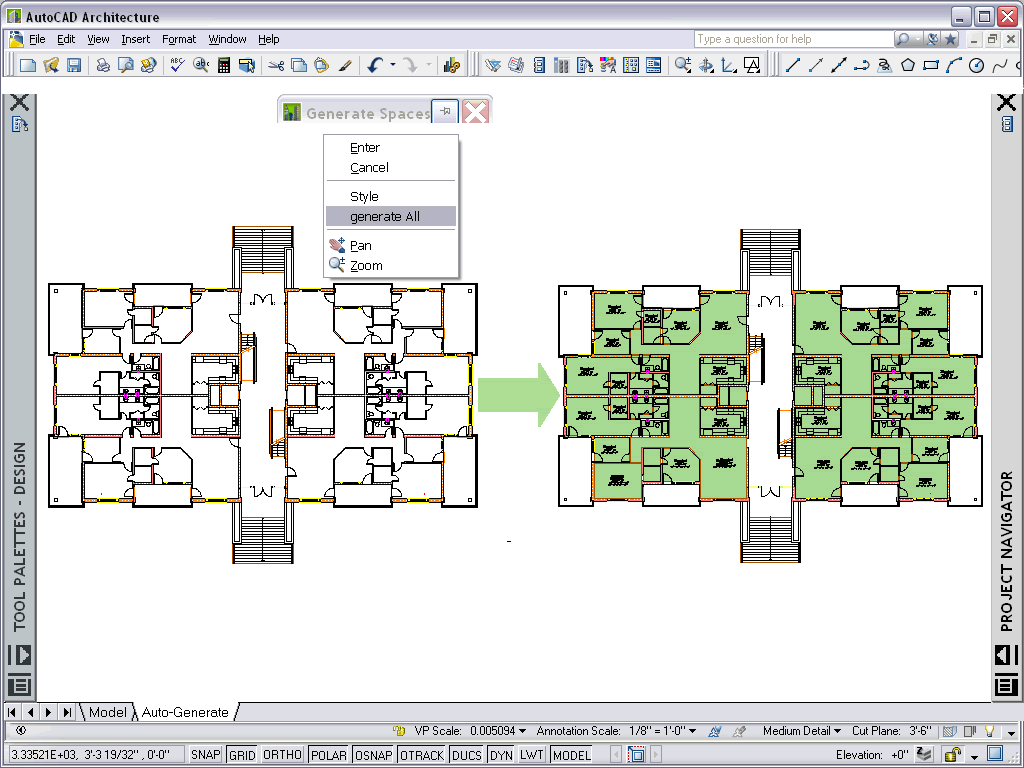
\includegraphics[width=.8\mycolumnwidth]{Introduccion_fundamentos/CAD.png}
\caption{\small Entorno de trabajo de una aplicaci�n CAD.}
\label{Fig:CAD} 
\end{figure}

El CAD puede resultar suficiente para desarrollar algunas tareas propias de los SIG, en particular las relacionadas con el dise�o cartogr�fico. No obstante, algunas circunstancias ponen de manifiesto las carencias de una herramienta CAD para sustituir completamente a un SIG, al tener requerimientos para los que esta no puede ofrecer una soluci�n. Entre estos requerimientos cabe citar los siguientes:
%
\begin{itemize}
\item An�lisis, modelizaci�n, y gesti�n avanzada de datos espaciales.
\item Trabajo con datos que cubren una gran superficie geogr�fica. Necesidad de utilizar diversos sistemas de proyecci�n.
\item Edici�n de datos por usuarios de distinto perfil y de modo concurrente.
\end{itemize}

Por su parte, las siglas AM/FM(\extr{Automated Mapping/Facilities Management})\footnote{Cartograf�a Automatizada/Gesti�n de Servicios} de uso poco habitual en nuestro idioma, hacen referencia a aplicaciones dise�adas para la gesti�n de infraestructuras generalmente de car�cter p�blico, tales como redes de alcantarillado, conducciones de gas o v�as de circulaci�n, entre otras. 

Las aplicaciones empleadas para estas tareas tienen dos bloques b�sicos: un bloque gr�fico de visualizaci�n y otro de gesti�n de datos. Este �ltimo almacena los atributos asociados a los elementos gr�ficos, que son principalmente de tipo lineal (tuber�as, redes de alumbrado, etc.). Otro tipo de elementos, tales como elementos poligonales, son dif�ciles de manejar en estos sistemas, ya que su dise�o obedece a las necesidades existentes en su �mbito de utilizaci�n, y estas se sit�an mayoritariamente alrededor de las infraestructuras lineales. Sin embargo, incluso con este tipo de elementos las capacidades de una aplicaci�n AM/FM no igualan a las de un SIG, ya que no incorporan otro tipo de informaci�n como la relativa a la topolog�a (que describiremos con detalle en el cap�tulo \ref{Tipos_datos}). Esto es as� debido a que el subsistema de an�lisis, fundamental en un SIG, no tiene presencia en estas herramientas, y por tanto sus caracter�sticas no incluyen aquellos componentes que sean necesarios exclusivamente para procesos de tipo anal�tico.

Puede decirse, por tanto, que este tipo de aplicaciones representa un subconjunto de los SIG, pues sus funcionalidades principales son m�s reducidas que las de estos, y su �mbito de aplicaci�n es menos generalista. En cierta medida, las aplicaciones AM/FM se asemejan tambi�n a las aplicaciones CAD, poniendo un �nfasis especial en la componente gr�fica, aunque con una mayor adaptaci�n a la naturaleza geogr�fica de la informaci�n con la que se trabaja.

Al contrario sin embargo de lo que sucede con las aplicaciones CAD, en la actualidad las labores propias asociadas a los productos AM/FM se pueden llevar a cabo en un SIG gen�rico, o bien en una adaptaci�n de este que tenga en consideraci�n las caracter�sticas particulares del �mbito de trabajo. En este sentido, la gesti�n de servicios no es una aplicaci�n m�s espec�fica que otras a la hora de emplear un SIG, y este en la actualidad engloba de forma casi completa las funcionalidades de una herramienta AM/FM.

%
\section{Componentes de un SIG}

Como ya hemos visto, en su concepci�n actual los SIG son sistemas complejos que integran una serie de distintos elementos interrelacionados. El estudio de todos y cada uno de estos elementos es el fundamento para el estudio global de los Sistemas de Informaci�n Geogr�fica, y de ese modo se aborda a lo largo de este libro, mostrando las propias caracter�sticas de cada elemento y los conceptos necesarios para entender las relaciones entre ellos.

Una forma de entender el sistema SIG es como formado por una serie de subsistemas, cada uno de ellos encargado de una serie de funciones particulares. Es habitual citar tres subsistemas fundamentales:

\begin{itemize}
	\item Subsistema de datos. Se encarga de las operaciones de entrada y salida de datos, y la gesti�n de estos dentro del SIG. Permite a los otros subsistemas tener acceso a los datos y realizar sus funciones en base a ellos.
	\item Subsistema de visualizaci�n y creaci�n cartogr�fica. Crea representaciones a partir de los datos (mapas, leyendas, etc.), permitiendo as� la interacci�n con ellos. Entre otras, incorpora tambi�n las funcionalidades de edici�n.
	\item Subsistema de an�lisis. Contiene m�todos y procesos para el an�lisis de los datos geogr�ficos.
\end{itemize}

La figura \ref{Fig:Relacion_subsistemas} muestra el esquema de estos tres subsistemas y su relaci�n.

\begin{figure}[h]   
\centering
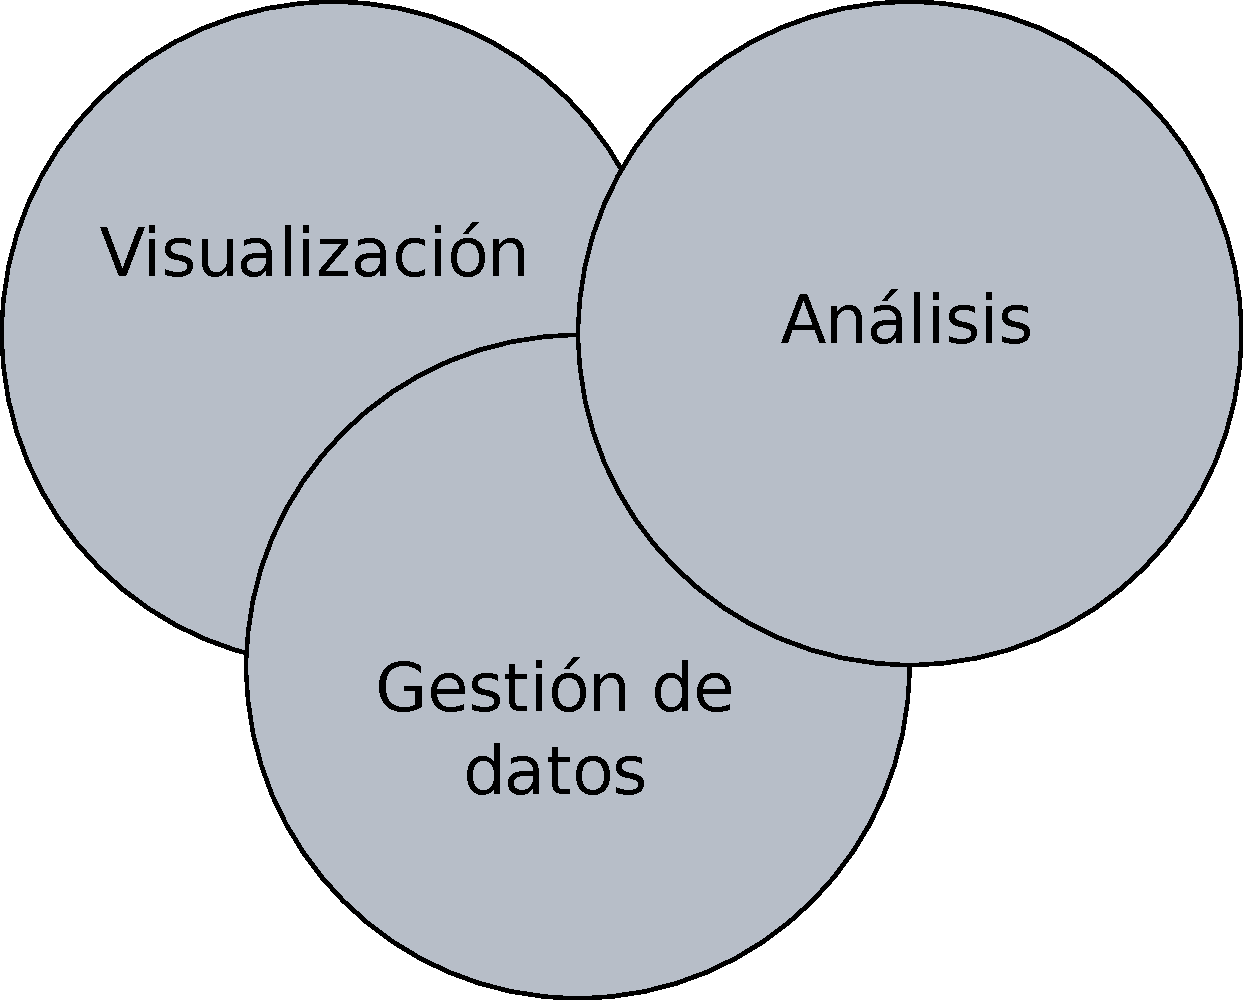
\includegraphics[width=.4\mycolumnwidth]{Introduccion_fundamentos/Relacion_subsistemas.pdf}
\caption{\small Esquema de un SIG con sus tres subsistemas fundamentales: datos, visualizaci�n y an�lisis}
\label{Fig:Relacion_subsistemas} 
\end{figure}

Para que un SIG pueda considerarse una herramienta �til y v�lida con car�cter general, debe incorporar estos tres subsistemas en cierta medida\cite{ESRI2003ESRI}.

Otra forma distinta de ver el sistema SIG es atendiendo a los elementos b�sicos que lo componen. Cinco son los elementos principales que se contemplan tradicionalmente en este aspecto (Figura \ref{Fig:Elementos_SIG}):

\begin{itemize}
 \item Datos. Los datos son la materia prima necesaria para el trabajo en un SIG, y los que contienen la informaci�n geogr�fica vital para la propia existencia de los SIG.
\item M�todos. Un conjunto de formulaciones y metodolog�as a aplicar sobre los datos.
\item Software. Es necesaria una aplicaci�n inform�tica que pueda trabajar con los datos e implemente los m�todos anteriores.
\item Hardware. El equipo necesario para ejecutar el software.
\item Personas. Las personas son las encargadas de dise�ar y utilizar el software, siendo el motor del sistema SIG.
\end{itemize}

\begin{figure}[h]   
\centering
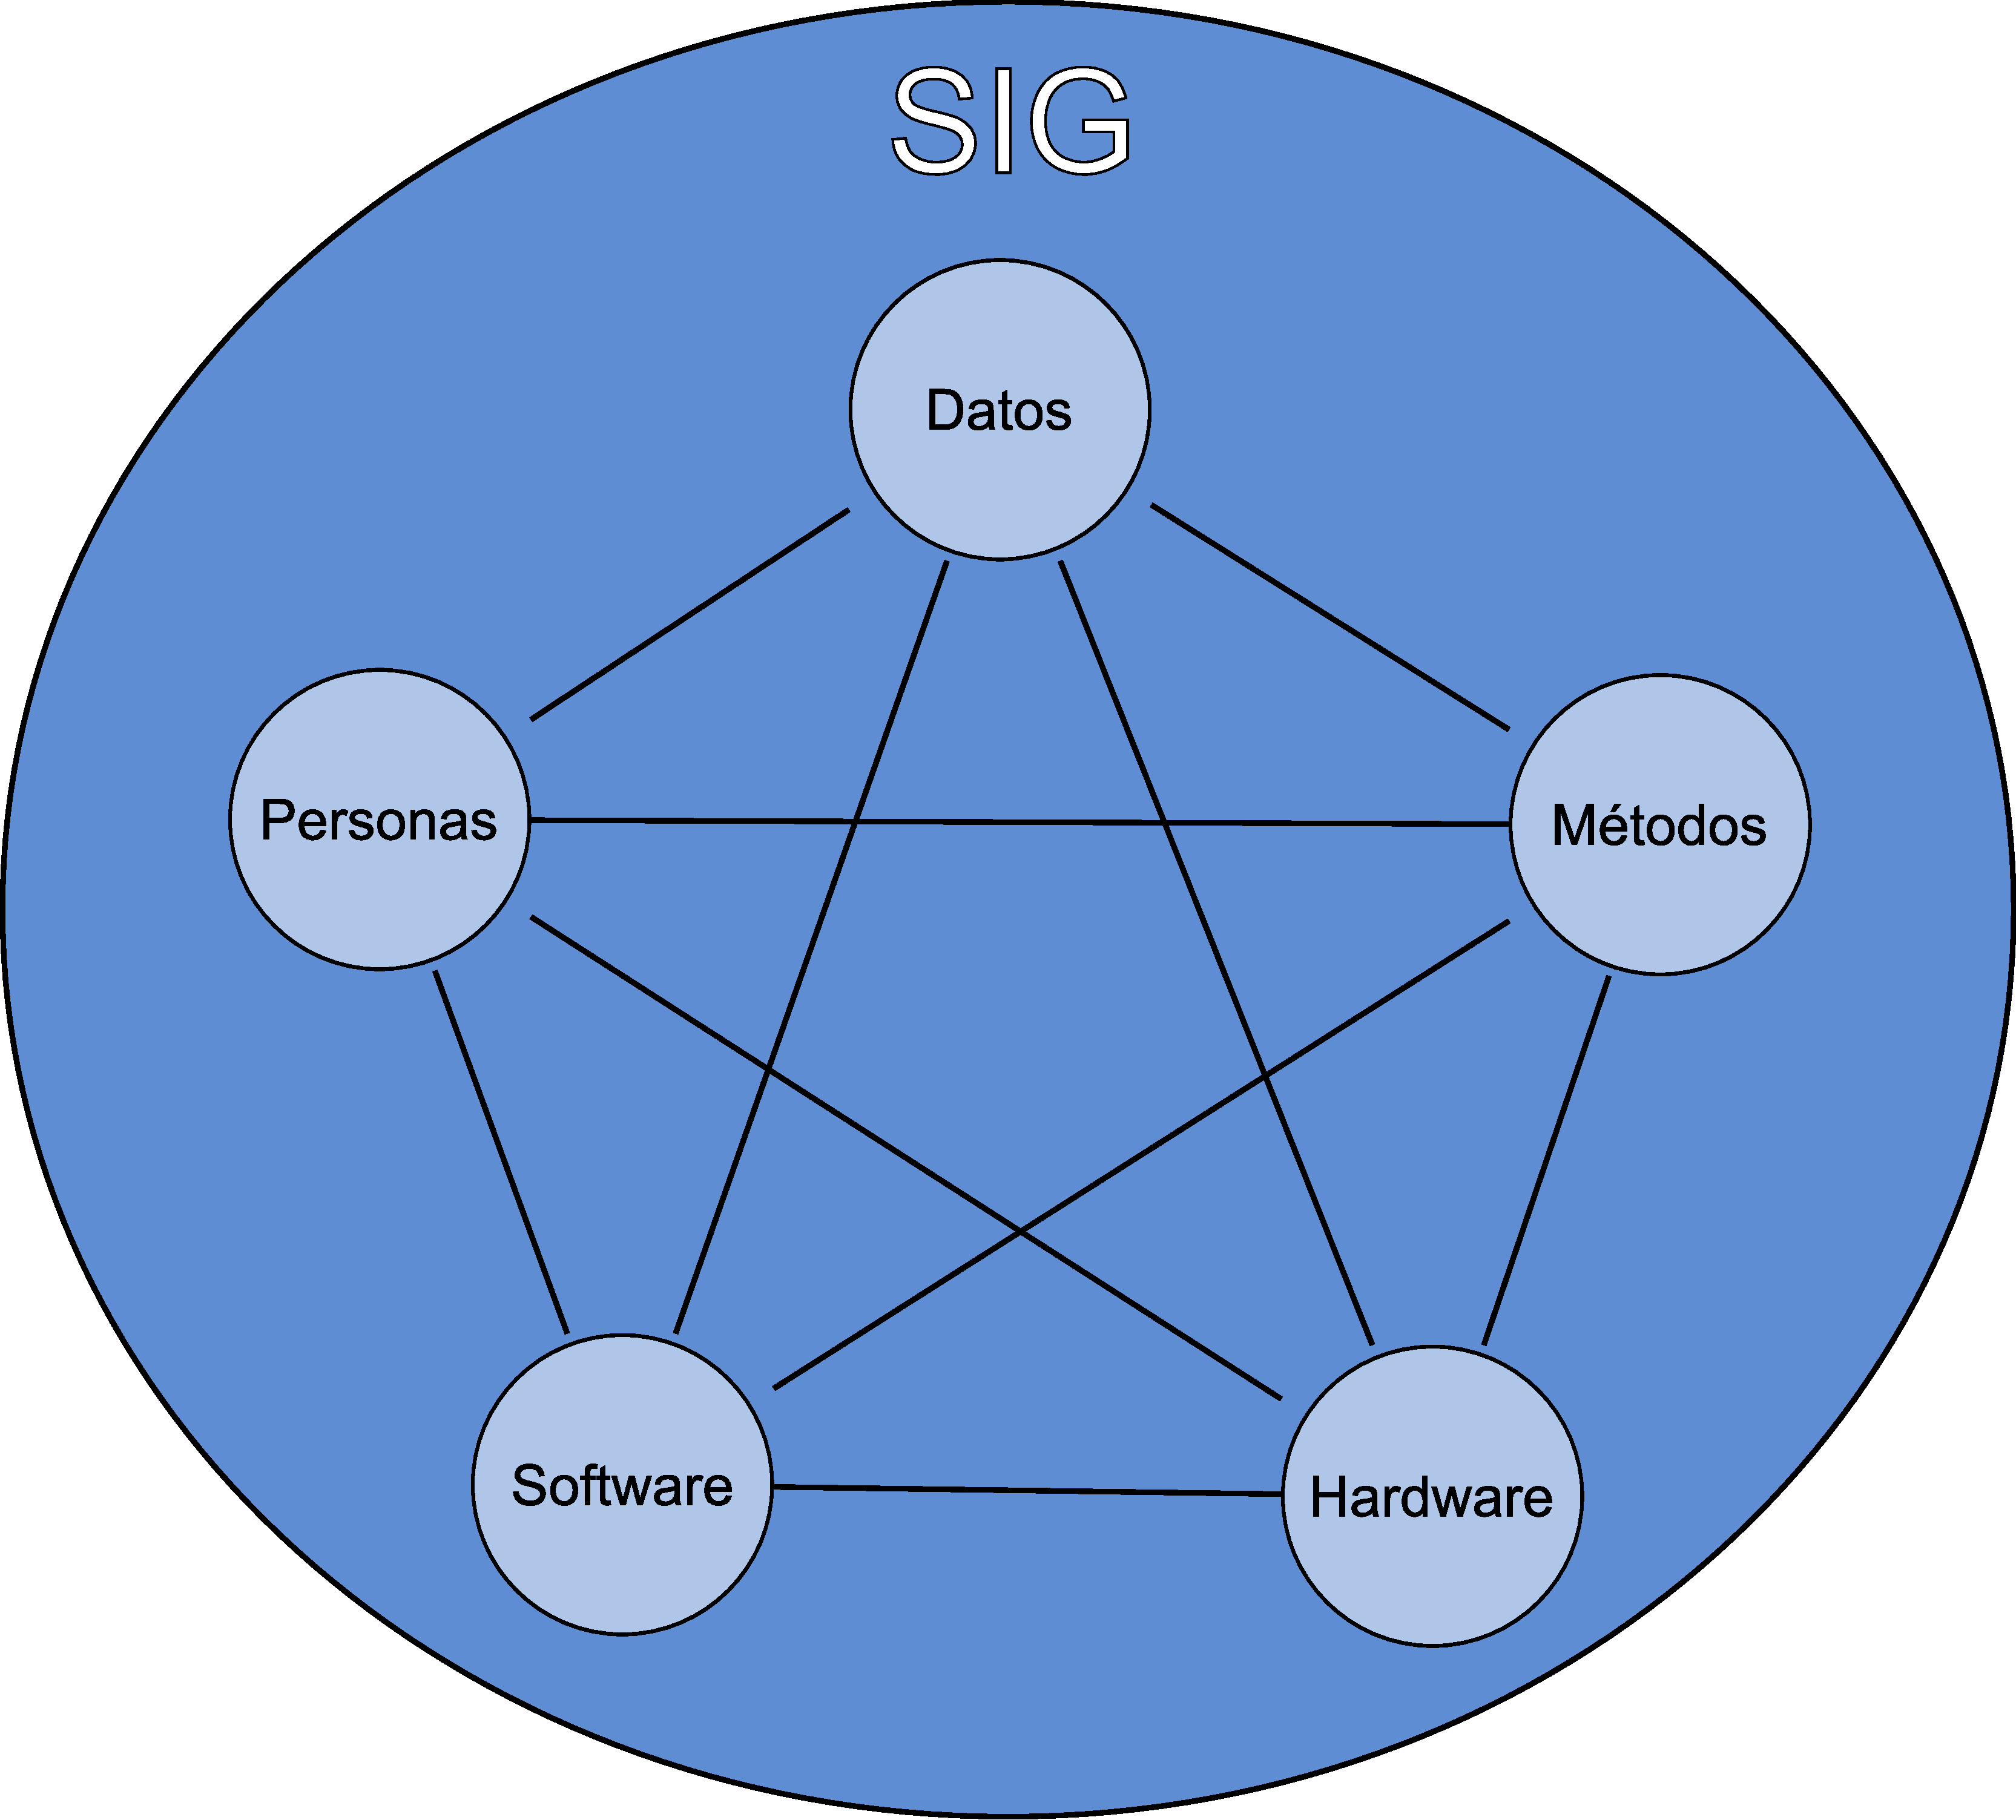
\includegraphics[width=.4\mycolumnwidth]{Introduccion_fundamentos/Elementos_SIG.pdf}
\caption{\small Elementos que forman el sistema SIG}
\label{Fig:Elementos_SIG} 
\end{figure}

Para el enfoque de esta obra, cada uno de los elementos anteriores tiene unas caracter�sticas propias que deben estudiarse. No obstante, el hardware no es un elemento especialmente particular en el caso de un SIG, y las aplicaciones SIG que encontramos actualmente en el mercado en todas sus variedades (que son las que el lector de este libro va a utilizar habitualmente) se ejecutan en su mayor�a sobre ordenadores personales sin requerimientos altamente espec�ficos. M�s a�n, la expansi�n de las tecnolog�as SIG ha alcanzado hoy en d�a otros �mbitos como las plataformas m�viles, haciendo de estas unas tecnolog�as poco espec�ficas en lo que a \extr{hardware} se refiere. Por esta raz�n, no es necesario tratar en detalle esta pieza del sistema SIG, siendo m�s adecuado tratar el resto de elementos, m�s caracter�sticos e importantes para el aprendizaje de los conceptos SIG y la descripci�n de estos.

Por su parte, las personas tienen importancia tanto de forma individual como en su conjunto, siendo diferentes las necesidades que plantean como usuarios y beneficiarios de un SIG. En la sociedad actual, las tecnolog�as y planteamientos colaborativos han calado hondo en el �mbito SIG, y la informaci�n geogr�fica es, por su propia naturaleza, propensa a ser compartida y utilizada por diferentes personas con fines muy distintos. Es por ello que el aspecto de mayor relevancia respecto a las personas como partes del sistema SIG es el de sus relaciones y su organizaci�n, siendo adem�s en este campo donde se han producido en mayor medida los �ltimos avances, y donde ha tenido lugar un cambio m�s profundo, no ya solo dentro de los SIG, sino tambi�n en otras tecnolog�as de similar �ndole.

Puede entenderse esto como un nuevo subsistema: el subsistema \emph{de gesti�n}, que es responsable de gestionar la interacci�n de los restantes y definir y controlar el marco en que esta tiene lugar.

Las personas a su vez dan forma a los distintos �mbitos de trabajo, definiendo estos en funci�n de sus necesidades. Puede tratarse el conjunto de campos de especializaci�n como un nuevo elemento del sistema SIG, en lugar de incorporarlo dentro de otro. 

Algunos autores proponen modificar el esquema cl�sico de cinco elementos para reflejar m�s correctamente la nueva realidad de los SIG. Por ejemplo, \cite{webGISEvolve} propone un esquema como el mostrado en la figura \ref{Fig:Elementos_SIG2}.

\begin{figure}[h]   
\centering
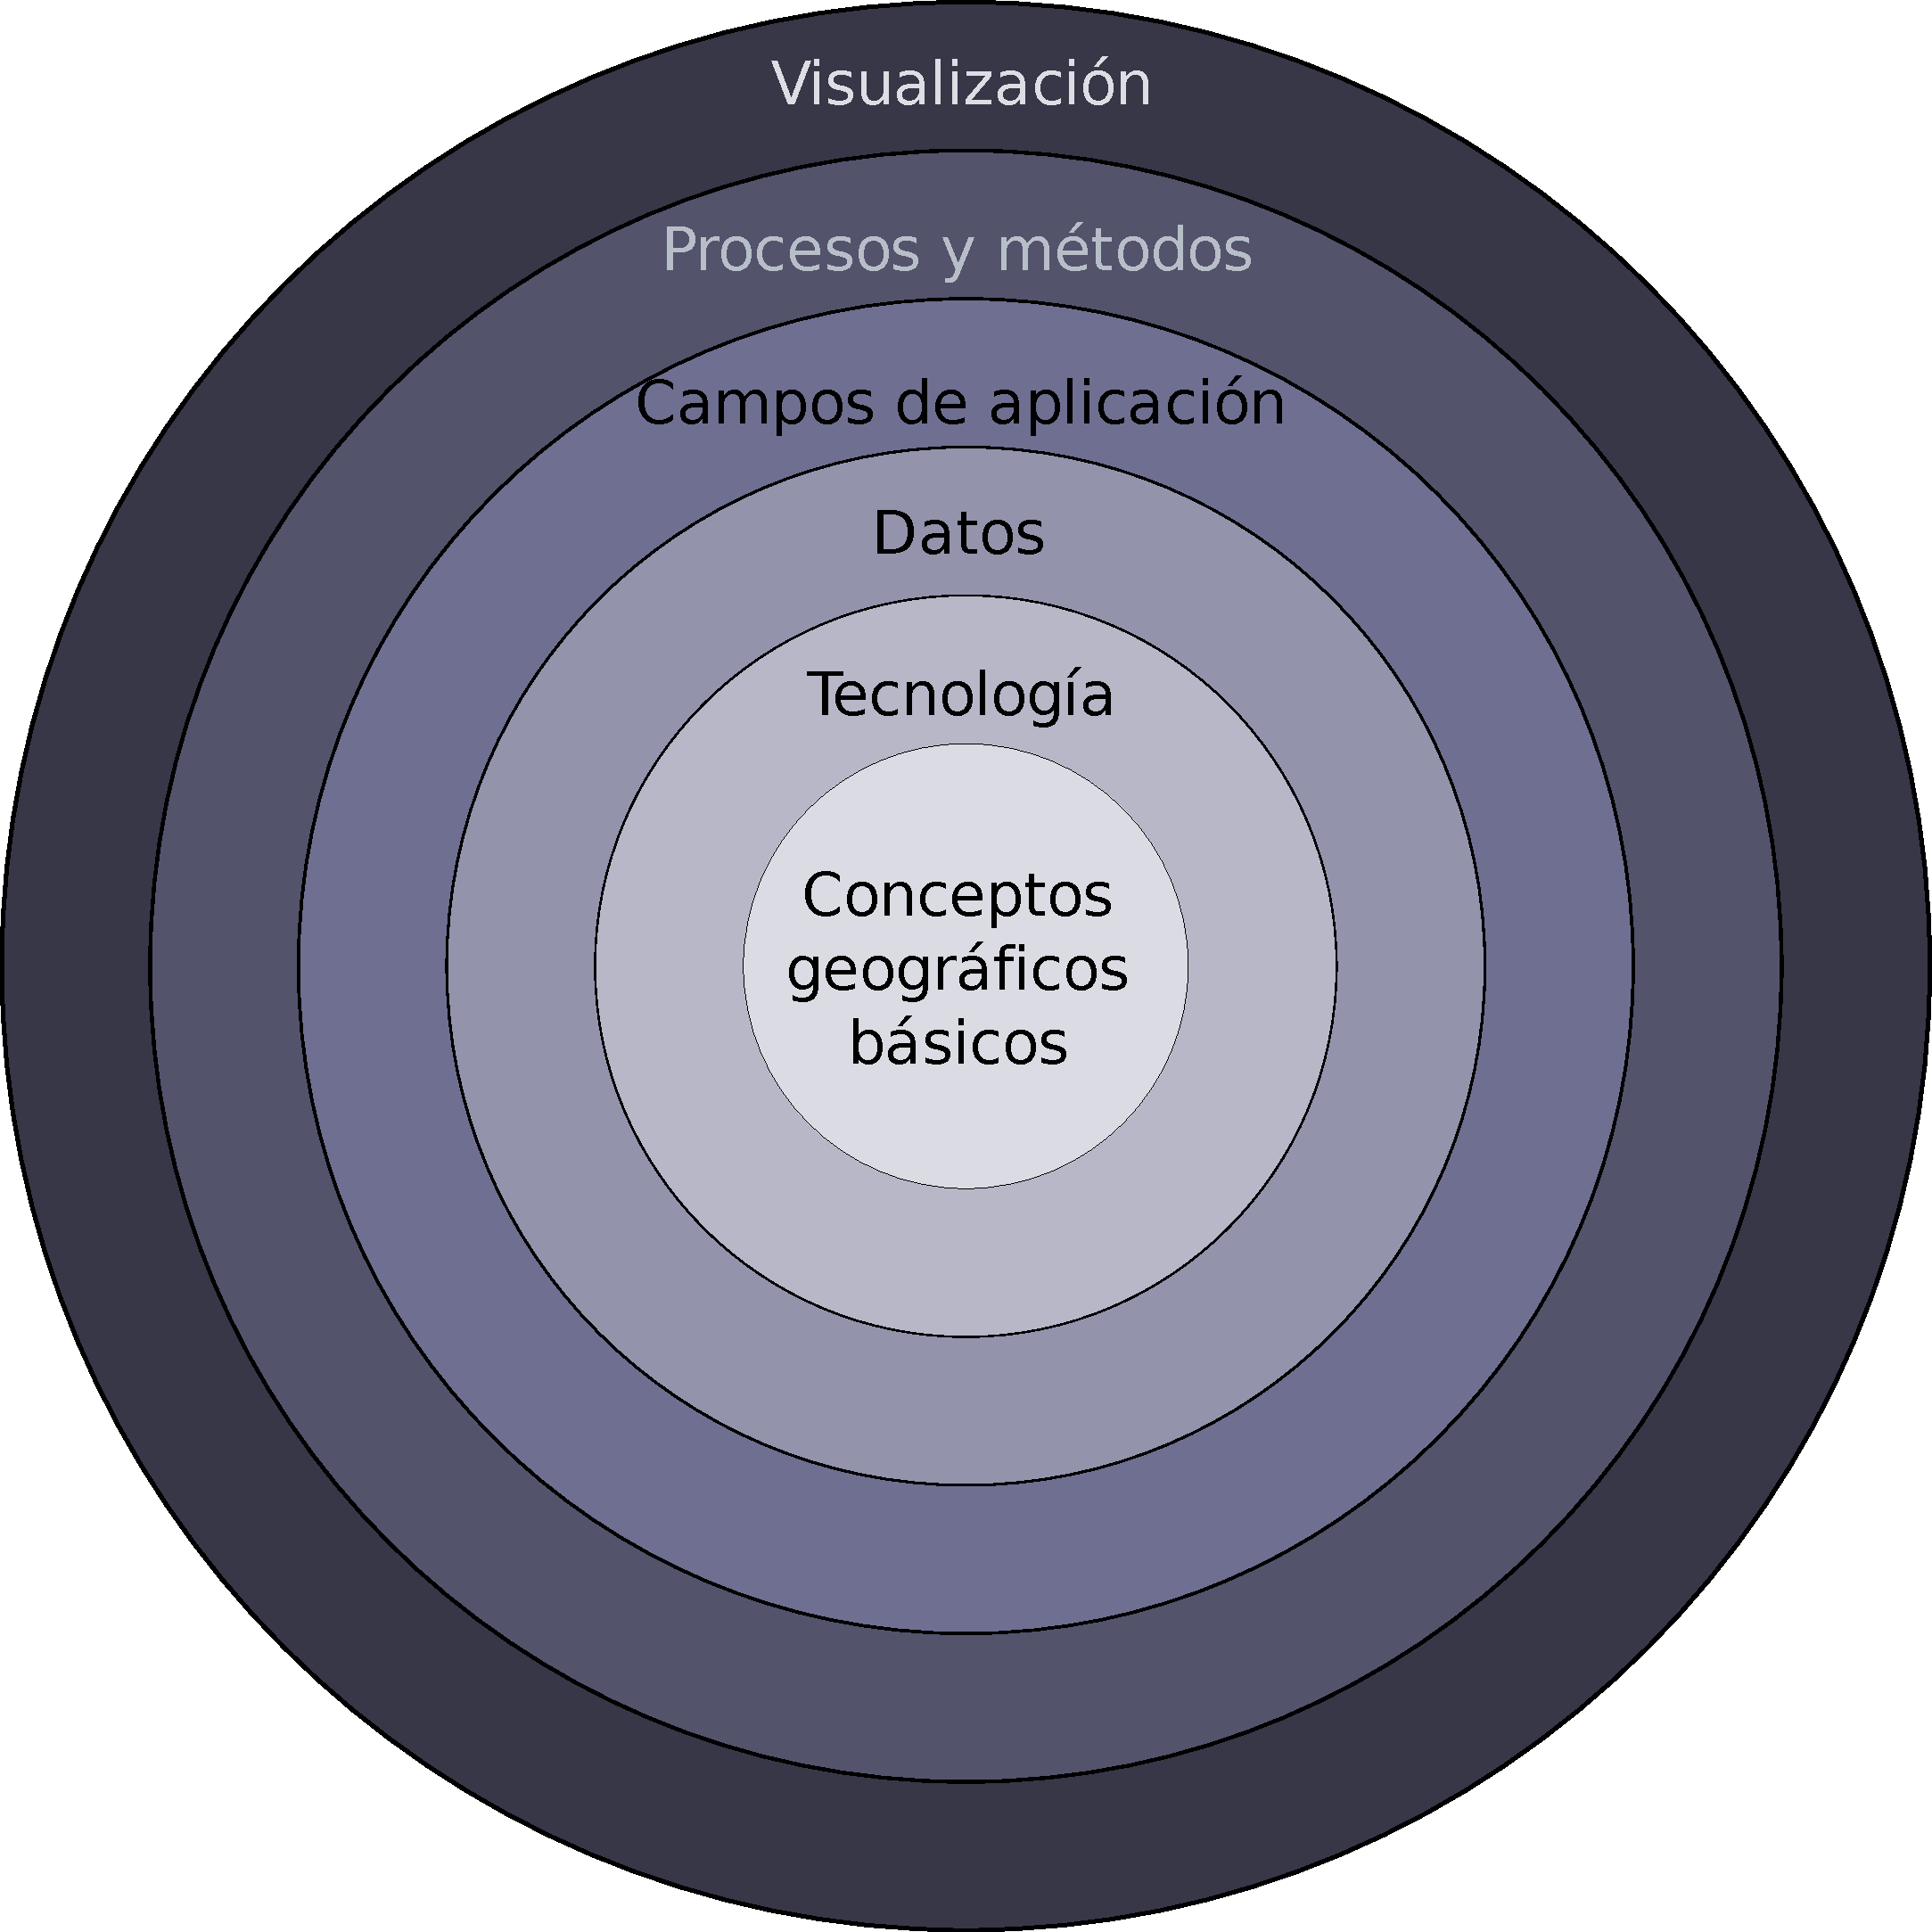
\includegraphics[width=.4\mycolumnwidth]{Introduccion_fundamentos/Elementos_SIG2.pdf}
\caption{\small Una divisi�n distinta del sistema SIG (seg�n \cite{webGISEvolve})}
\label{Fig:Elementos_SIG2} 
\end{figure}

La incorporaci�n de la visualizaci�n es una diferencia notable con respecto al esquema cl�sico. En realidad, y si volvemos a ese enfoque basado en subsistemas, el subsistema de visualizaci�n resulta de enorme importancia en un SIG, siendo pese a ello habitual que no sea tratado con la suficiente profundidad en textos dedicados a los SIG desde un punto de vista gen�rico. Precisamente por no ser considerado un elemento independiente, no se le concede la necesaria atenci�n como parte que debe estudiarse al tratar la disciplina de los SIG.

Esto contrasta con el hecho de que, a pesar de que las capacidades de los SIG son mucho m�s amplias que las relacionadas con la visualizaci�n, muchos usuarios usan estas por encima de las restantes, desconociendo incluso en muchos casos gran parte de las otras capacidades que un SIG puede brindarles. Correcto o no, desde el punto de vista del usuario medio, las capacidades de visualizaci�n est�n en primera l�nea del conjunto de funcionalidades de un SIG.

Abordar el estudio de un SIG acudiendo al esquema cl�sico de cinco elementos deja de lado la visualizaci�n, en cuanto que la engloba como una funcionalidad derivada de dichos elementos en su conjunto pese a que esta tiene unas caracter�sticas peculiares en el entorno de un SIG y una vital importancia en la concepci�n actual de este. Es decir, el esquema de partes de un SIG no resulta el m�s adecuado para estructurar el estudio de los SIG, al menos en lo que respecta a la visualizaci�n como parte fundamental de estos.

El objetivo de este libro es tratar con suficiente detalle y rigor todos los aspectos fundamentales de un SIG, incluyendo, por supuesto, la visualizaci�n de datos geogr�ficos. Para ello, es conveniente tratar tambi�n esta desde un punto de vista te�rico, detallando los fundamentos en los que se basa y que, pese a ser de vital importancia para el uso de un SIG, son ignorados frecuentemente. 

Con todo lo anterior, resulta m�s conveniente para su estudio pr�ctico adoptar una evoluci�n del esquema cl�sico de cinco elementos, y establecer unos nuevos componentes, cada uno de los cuales act�a como un pilar conceptual sobre es que ha de sustentarse es estudio de la disciplina de los SIG. Estos componentes son cinco:

\begin{itemize}
 \item Datos.
\item Procesos. M�todos enfocados al an�lisis de los datos.
\item Visualizaci�n. M�todos y fundamentos relacionados con la representaci�n de los datos. 
\item Tecnolog�a. \extr{Software} y \emph{hardware} SIG
\item Factor organizativo. Engloba los elementos relativos a la coordinaci�n entre personas, datos y tecnolog�a, o la comunicaci�n entre ellos, entre otros aspectos.
\end{itemize}
%
A modo de introducci�n, se describen a continuaci�n algunas ideas b�sicas de cada uno de estos componentes. Posteriormente, cada uno de ellos ser� tratado en detalle en una parte completa de este libro.

Aunque no lo consideraremos como una parte del sistema SIG, el conjunto de �mbitos especializados de aplicaci�n merece tambi�n atenci�n separada, pues todo usuario de SIG deber� situarse en uno de ellos a la hora de llevar a cabo su trabajo. Por ello, dedicaremos igualmente una parte del libro a tratar las principales �reas de aplicaci�n de los SIG.

\subsection{Datos}

Los datos son necesarios para hacer que el resto de componentes de un SIG cobre sentido y puedan ejercer su papel en el sistema. La informaci�n geogr�fica, la verdadera raz�n de ser los SIG, reside en los datos, y es por ello que el conocimiento exhaustivo de los datos y su naturaleza resulta obligado para una buena comprensi�n los propios SIG.

Son muchas las facetas de los datos que deben estudiarse, y todas ellas con una gran importancia. Por un lado, es necesario conocer las caracter�sticas fundamentales del dato geogr�fico que utilizamos en un SIG, es decir, su forma y sus propiedades. De ellas dependen, por ejemplo, los procesos que podremos o no realizar con los datos, y en general todo cuanto podemos esperar de ellos.

Prescindiendo del hecho de que se trata de un dato geogr�fico, es relevante conocer c�mo los datos se gestionan y almacenan en un entorno digital, aspectos de corte puramente inform�tico que desarrolla la disciplina de la gesti�n de bases de datos. Cuando las ideas fundamentales al respecto se aplican al caso particular de los datos geogr�ficos, surgen conceptos que resultan b�sicos para un buen uso de un SIG, y que adem�s van siendo cada vez m�s relevantes a medida que los vol�menes de datos de que se dispone van aumentando. 

Al igual que aumenta el volumen de datos, lo hacen los or�genes de estos y las formas en que la informaci�n geogr�fica puede recogerse. Un aspecto clave para una utilizaci�n correcta de un SIG es saber integrar datos de distinta procedencia, para lo cual es vital entender c�mo esta afecta a las propias caracter�sticas de dichos datos.

Otros elementos tales como la calidad de los datos, la cual cobra cada d�a m�s importancia, ser�n tratados igualmente junto a los anteriores en una parte espec�ficamente dedicada a los datos, probablemente una de las m�s importantes dentro de este libro.

\subsection{Procesos}

El an�lisis es una las funcionalidades b�sicas de los SIG, y una de las razones fundamentales que llevaron al desarrollo de estos. Un ordenador es una herramienta con enorme capacidad de c�lculo, y esta puede aplicarse a los datos espaciales para obtener resultados de muy diversa �ndole.

En mayor o menor medida, un SIG siempre incorpora una serie de formulaciones que permiten la obtenci�n de resultados y el an�lisis de los datos espaciales. Estas formulaciones representan procesos que pueden ser sumamente sencillos o enormemente complejos, y que pueden resultar de aplicaci�n en uno u otro campo, o incluso con car�cter general. Su origen puede ser muy variado, y no derivan  necesariamente del �mbito puro de la geograf�a, sino que pueden ir desde simples consultas o mediciones a elaborados modelos que empleen datos de variables muy numerosas y arrojen resultados complejos. La estad�stica, entre otras ciencias, puede aportar al �mbito SIG muchas de sus ideas, y estas, adaptadas al marco de la informaci�n georreferenciada, constituir en el SIG un nuevo conjunto de procesos de an�lisis.

Las ventajas de la incorporaci�n de todos estos procesos en una �nica herramienta, el SIG, van desde la automatizaci�n de tareas a la aparici�n de nuevos procesos que, aprovechando la gran capacidad de c�mputo de la plataforma en la que se ejecuta el SIG, producen resultados que no podr�an ser obtenidos de otro modo. Bien sea por la complejidad propia de los procesos o por el nivel de precisi�n al que se trabaja, existen muchos procesos que mediante el uso de cartograf�a cl�sica y sin el apoyo de medios informatizados no pueden realizarse. El SIG abre un campo de actuaci�n en el que la practica totalidad de ideas y formulaciones de an�lisis pueden plasmarse y aplicarse con car�cter pr�ctico.


\subsection{Visualizaci�n}

Cualquier tipo de informaci�n puede ser representada de forma gr�fica, lo cual habitualmente facilita la interpretaci�n de dicha informaci�n o parte de esta. Gran parte de las caracter�sticas de la informaci�n (por ejemplo, la presencia de patrones sistem�ticos), son m�s f�ciles de estudiar cuando se apoyan sobre alg�n elemento visual, pues este a�ade un nuevo punto de vista.

En el caso particular de la informaci�n geogr�fica, la visualizaci�n no solo es una forma m�s de trabajar con esa informaci�n, sino que resulta la forma principal, no ya por ser la que en general hace m�s f�cil e intuitivo el tratamiento de esa informaci�n, sino porque es aquella a la que estamos m�s acostumbrados. La informaci�n geogr�fica tiene una inherente naturaleza visual, ya que el espacio en s� es entendido de forma gr�fica por el ser humano. Junto a esto, no debemos olvidar que la informaci�n geogr�fica se ha almacenado de forma tradicional de modo tambi�n visual, a trav�s de mapas. Un mapa es en s� una representaci�n visual de la informaci�n geogr�fica.

Al contrario que un mapa, que de por s� es de naturaleza gr�fica, en un SIG trabajamos con datos de tipo puramente num�rico, ya que es as� como el ordenador puede manejarlos, y la informaci�n geogr�fica debe almacenarse de este modo, como veremos con detalle en el cap�tulo \ref{Tipos_datos}. Para poder presentar una utilidad similar a la de un mapa en lo que a la presentaci�n de la informaci�n respecta, un SIG debe incluir capacidades que generen representaciones visuales a partir de esos datos num�ricos, aprovechando en la medida de lo posible las propias capacidades del medio inform�tico en que se trabaja para hacer estas representaciones m�s potentes como transmisoras de informaci�n. 

Es deseable igualmente que el SIG sea capaz de generar cartograf�a cl�sica, y que incorpore m�todos para el dise�o cartogr�fico y la creaci�n de mapas impresos, pues estos no pierden su vigencia pese a la existencia de los SIG.

La visualizaci�n de la informaci�n geogr�fica se rige por los mismos conceptos y principios que se emplean para la confecci�n de cartograf�a impresa, y estos deben ser conocidos por el usuario de SIG, ya que una de las tareas de este es el dise�o cartogr�fico y las preparaci�n de los elementos de visualizaci�n para poder realizar su trabajo sobre las representaciones creadas. A los conceptos tradicionales hay que sumar algunas ideas nuevas, ya que un SIG es capaz de generar representaciones m�s avanzadas (por ejemplo, representaciones tridimensionales). A esto hay que sumar la presencia de un elemento caracter�stico y de gran importancia como es la elevada interactividad que toda representaci�n gr�fica lleva asociada dentro de un SIG, y que constituye una gran diferencia frente al car�cter est�tico de la cartograf�a cl�sica.

Por todo ello, la visualizaci�n debe considerarse como un componente fundamental del sistema SIG en su concepci�n actual, y particularmente uno con especial inter�s desde el punto de vista del usuario directo de tecnolog�as SIG.

\subsection{Tecnolog�a}

Incluimos en este elemento tanto el \emph{hardware} sobre el que se ejecutan las aplicaciones SIG, como dichas aplicaciones, es decir el \emph{software} SIG. Ambos forman un binomio tecnol�gico en el que encontramos diversas alternativas, y que se enriquece diariamente con la r�pida evoluci�n del mercado tecnol�gico.

En lo que a \emph{hardware} respecta, es el elemento f�sico del sistema SIG, y conforma la plataforma sobre la que tiene lugar el trabajo con un SIG. La utilizaci�n de un SIG hoy en d�a se puede llevar a cabo en ordenadores personales o estaciones de trabajo, y ya sea de forma individual o en una arquitectura cliente--servidor m�s compleja. Estas �ltimas han cobrado importancia muy r�pidamente en los �ltimos tiempos, especialmente en lo que al acceso a datos se refiere. Veremos m�s adelante como esto tambi�n ha tenido influencia en otros componentes del sistema SIG, principalmente en el factor organizativo.

Adem�s de la propia plataforma, el \emph{hardware} incluye una serie de perif�ricos para tareas m�s concretas. De uso habitual en el trabajo con SIG son los perif�ricos para entrada de datos geogr�ficos y la creaci�n de cartograf�a. Las tabletas digitalizadoras son la forma m�s habitual dentro del primer grupo (las veremos con m�s detalle en el apartado \ref{heads-down}), mientras que \emph{plotters}\index{Plotter} e impresoras son empleados para la creaci�n cartogr�fica, requiri�ndose generalmente un mayor formato que para otros usos.

Mas recientemente, la aparici�n de Sistemas de Navegaci�n Global\index{Sistemas de Navegaci�n Global} como el GPS\index{GPS} (que pueden a su vez considerarse como otro tipo de perif�ricos) ha creado una parcela tecnol�gica con gran relaci�n con los SIG, convirtiendo a estos en herramientas ideales para la gesti�n de los datos de dichos sistemas. Incluso, la combinaci�n de SIG y GPS sobre un �nico elemento de hardware ha dado lugar a herramientas como los navegadores GPS, que han supuesto un hito no solo desde el punto de vista t�cnico, sino tambi�n desde un enfoque social, pues acercan las tecnolog�as SIG a usuarios no expertos.

Por su parte, el \emph{software} es el encargado de operar y manipular los datos. El software SIG tambi�n ha sufrido una gran evoluci�n, y bajo el paraguas de esa denominaci�n encontramos desde las aplicaciones cl�sicas que permiten visualizar, gestionar y analizar los datos geogr�ficos, hasta herramientas m�s especializadas que se centran en alguno de estos campos, o bien componentes que pueden incluso pasar a formar parte de otras aplicaciones fuera del �mbito SIG, pero que puntualmente requieren algunas de sus funcionalidades, especialmente las relacionadas con la visualizaci�n de cartograf�a digital.

\subsection{Factor organizativo}

El sistema SIG requiere una organizaci�n y una correcta coordinaci�n entre sus distintos elementos. El factor organizativo ha ido progresivamente ganando importancia dentro del entorno SIG, a medida que la evoluci�n de estos ha ido produciendo un sistema m�s complejo y un mayor n�mero de intrarelaciones e interrelaciones entre los distintos componentes que lo forman.

Especialmente importante es la relaci�n entre las personas que forman parte del sistema SIG, as� como la relaci�n de todos los elementos con los datos, sobre los cuales act�an de un modo u otro. Ello ha propiciado la aparici�n de, entre otros, elementos que pretenden estandarizar los datos y gestionar estos adecuadamente.

Cuando los SIG se encontraban en sus etapas de desarrollo iniciales y eran meras herramientas para visualizar datos y realizar an�lisis sobre ellos, cada usuario tenia sus propios datos con los cuales trabajaba de forma independiente del resto de usuarios, incluso si estos llevaban a cabo su trabajo sobre una misma �rea geogr�fica y estudiando las mismas variables. Hoy en d�a, la informaci�n no se concibe como un elemento privado de cada usuario, sino como un activo que ha de gestionarse, y del que deriva toda una disciplina completa.La aplicaci�n de esta disciplina es la base de algunos de los avances m�s importantes en la actualidad, teniendo implicaciones no ya solo t�cnicas sino tambi�n sociales en el �mbito de los SIG.

Asimismo, las necesidad de gesti�n de los datos y la propia complejidad de un SIG, provocan ambas que no exista un perfil �nico de persona involucrada en el sistema SIG, sino varias en funci�n de la actividad que desarrollen. Al usuario cl�sico de SIG se unen las personas responsables de gestionar las bases de datos, las encargadas de dise�ar la arquitectura de un SIG cuando este se establece para un uso conjunto por parte de toda una organizaci�n o grupo de mayor entidad. Dentro de las personas que participan en un SIG, el usuario directo es el eslab�n �ltimo de una cadena que incluye igualmente a otros profesionales con roles bien distintos.

Incluso atendiendo �nicamente a los usuarios, tambi�n entre estos existen diferentes perfiles, y las comunidades de usuarios no expertos juegan en la actualidad un importante papel en el mundo del SIG. Esta situaci�n, a su vez, requiere elementos organizativos importantes. Con la popularizaci�n y bajo coste de las unidades GPS y la aparici�n de la denominada Web 2.0, el SIG ha llegado a usuarios no especializados, los cuales utilizan estas herramientas para la creaci�n y uso de su propia cartograf�a, dentro de lo que se conoce como VGI (\emph{Volunteered Geographic Information}\footnote{Informaci�n geogr�fica creada voluntariamente}) \cite{goodchildVGI}. El t�rmino \emph{Neogeograf�a}, de reciente creaci�n, hace referencia a este uso de los SIG y otras herramientas asociadas por parte de grupos de usuarios no especializados.

En definitiva, resulta necesario gestionar correctamente la complejidad del sistema SIG, y esta gesti�n se ha convertido ya en un elemento fundamental dentro del entorno SIG actual, por lo que debe ser estudiada igualmente.

\section{Resumen}

En este cap�tulo hemos presentado los SIG como herramienta para el manejo general de informaci�n geogr�fica, fundamental para trabajar hoy en d�a con todo tipo de informaci�n georreferenciada. Un SIG es un sistema compuesto por cinco piezas fundamentales: datos, tecnolog�a, procesos, visualizaci�n y factor organizativo. Cada una de ellas cumple un papel determinado dentro del sistema SIG, el cual se caracteriza fundamentalmente por su naturaleza integradora. 

Existen otras herramientas y tecnolog�as que pueden en principio asemejarse a los SIG, pero que realmente no comparten con estos su capacidad de integrar bajo un marco com�n una serie completa de elementos y disciplinas, siendo esta la verdadera propiedad que define a los SIG.

Todo el conjunto de conocimientos sobre los cuales se asientan los SIG conforman la denominada Ciencia de la Informaci�n Geogr�fica. Bajo esta denominaci�n se recogen todos los temas a tratar en esta obra.

%\bibliographystyle{unsrt}
%\bibliography{../../Libro_SIG}


\chapter{Historia de los SIG}\label{Historia}

\begin{keypoints}
�Cu�ndo y d�nde se desarrollo el primer SIG? $\bullet$ �C�mo han evolucionado los SIG desde sus or�genes hasta nuestros d�as? $\bullet$ �Qu� etapas pueden diferenciarse? $\bullet$ �C�mo ha evolucionado la recogida de datos utilizados en un SIG? $\bullet$ �Qu� eventos han marcado la historia de los SIG? $\bullet$ �C�mo ha afectado al desarrollo de los SIG la evoluci�n de otras tecnolog�as y disciplinas?
\end{keypoints}

\bigskip

\begin{intro}
Antes de comenzar a estudiar en profundidad los Sistemas de Informaci�n Geogr�fica y sus elementos constituyentes, as� como la ciencia que definen, es conveniente ver c�mo se ha llegado hasta la situaci�n actual a partir de los esfuerzos llevados a cabo en diversas direcciones. Estudiar la evoluci�n y desarrollo de los SIG es ciertamente importante, en la medida en que nos encontramos ante una disciplina compleja que se nutre de muchas fuentes distintas. En este cap�tulo recorreremos el camino desde los primeros programas que establecieron las bases para el concepto de SIG, hasta llegar a la concepci�n moderna de este. De esta manera, ser� m�s sencillo entender m�s adelante el porqu� de cada una de las partes de un SIG, su funcionalidad y su raz�n de ser.
\end{intro}

\section{Introducci�n}

El desarrollo sufrido por los SIG desde sus or�genes hasta nuestros d�as es enorme. La popularizaci�n de las tecnolog�as y los esfuerzos de desarrollo llevados a cabo por un amplio abanico de ciencias beneficiarias de los SIG, todos han contribuido a redefinir la disciplina e incorporar elementos impensables entonces. No obstante, los componentes principales que identifican el n�cleo principal de un SIG se mantienen a lo largo de todo ese desarrollo, y es su aparici�n la que define el momento inicial en el que podemos situar el origen de los SIG.

Este momento surge al inicio de la d�cada de los sesenta como resultado de unos factores que convergen para dar lugar al desarrollo de los primeros SIG. Estos factores son principalmente dos: la necesidad creciente de informaci�n geogr�fica y de una gesti�n y uso �ptimo de la misma, y la aparici�n de los primeros computadores. 

Estos mismos factores son los que desde entonces han seguido impulsando el avance de los SIG, ya que el inter�s en el estudio y conservaci�n del medio se incrementa paulatinamente tambi�n hoy en d�a, y ello crea una situaci�n ideal para la evoluci�n de las t�cnicas y herramientas empleadas, muy particularmente los SIG.

\section{Los or�genes}

Las bases para la futura aparici�n de los SIG las encontramos algunos a�os antes de esa d�cada de los sesenta, con el desarrollo de nuevos enfoques en cartograf�a que parecen predecir las necesidades futuras que un manejo informatizado de esta traer�. Los trabajos desarrollados por John K.Wright\index{Wright, John K.} en la Sociedad Geogr�fica Americana\index{Sociedad Geogr�fica Americana}, en especial la publicaci�n de su obra \emph{Elements of Cartography} en 1953\index{Elements of Cartography}, son particularmente importantes. Obras como esta van ampliando el campo de la geograf�a cuantitativa hasta que este alcanza un nivel donde puede plantearse, una vez que la inform�tica alcanza una cierta madurez, la uni�n de ambas disciplinas.

La primera experiencia relevante en esta direcci�n la encontramos en 1959, cuando Waldo Tobler\index{Tobler, Waldo} define los principios de un sistema denominado MIMO (map in--map out)\index{MIMO}\index{Map in-map out} con la finalidad de aplicar los ordenadores al campo de la cartograf�a. En �l, establece los principios b�sicos para la creaci�n de datos geogr�ficos, su codificaci�n, an�lisis y representaci�n dentro de un sistema informatizado. Estos son los elementos principales del \emph{software} que integra un SIG, y que habr�n de aparecer en todas las aplicaciones desarrolladas desde ese momento.

El primer Sistema de Informaci�n Geogr�fica formalmente desarrollado aparece en Canad�, al auspicio del Departamento Federal de Energ�a y Recursos. Este sistema, denominado CGIS (Canadian Geographical Information Systems)\index{CGIS}, fue desarrollado a principios de los 60 por Roger Tomlinson\index{Tomlinson, Roger}, quien dio forma a una herramienta que ten�a por objeto el manejo de los datos del inventario geogr�fico canadiense y su an�lisis para la gesti�n del territorio rural. El desarrollo de Tomlinson es pionero en este campo, y se considera oficialmente como el nacimiento del SIG. Es en este momento cuando se acu�a el t�rmino, y Tomlinson es conocido popularmente desde entonces como <<el padre del SIG>>.

La aparici�n de estos programas no solo implica la creaci�n de una herramienta nueva, sino tambi�n el desarrollo de t�cnicas nuevas que hasta entonces no hab�an sido necesarias. La m�s importante de ellas es la codificaci�n y almacenamiento de la informaci�n geogr�fica, un problema en absoluto trivial que entonces era clave para lograr una usabilidad adecuada del \emph{software}. El trabajo de Guy Morton\index{Morton!Guy} con el desarrollo de su \emph{Matriz de Morton}\index{Matriz!de Morton}\index{Morton!Matriz de}\footnote{Veremos con algo m�s de detalle este concepto en el cap�tulo \ref{Tipos_datos}} juega un papel primordial\cite{Foresman1998Prentice}, superando las deficiencias de los equipos de entonces, tales como la carencia de unidades de almacenamiento con capacidad de acceso aleatorio, que dificultaban notablemente el manejo y an�lisis de las bases de datos.

Simult�neamente a los trabajos canadienses, se producen desarrollos en Estados Unidos, en el seno del Harvard Laboratory\index{Harvard Laboratory}, y en el Reino Unido dentro de la Experimental Cartography Unit\index{Experimental Cartography Unit}. Ambos centros se erigen tambi�n como principales desarrolladores de \emph{software} para la producci�n, manejo y an�lisis de informaci�n geogr�fica durante aquellos a�os.

En el Harvard Laboratory, ve la luz en 1964 SYMAP\index{SYMAP}, un aplicaci�n que permit�a la entrada de informaci�n en forma de puntos, l�neas y �reas, lo cual se corresponde a grandes rasgos con el enfoque que conocemos hoy en d�a como \emph{vectorial}. En la imagen \ref{Fig:SYMAP} puede verse que los resultados cartogr�ficos de este \emph{software} son a�n de poca calidad. No obstante, el inter�s que despertaron las novedosas capacidades del programa para la generaci�n de cartograf�a impuls� el desarrollo posterior y la evoluci�n hacia sistemas m�s avanzados.

En 1969, utilizando elementos de una versi�n anterior de SYMAP, David Sinton\index{Synton, David}, tambi�n en el Harvard Laboratory, desarrolla GRID\index{GRID}, un programa en el que la informaci�n es almacenada en forma de cuadr�culas. Hasta ese momento, la estructura de cuadr�culas regulares era solo utilizada para las salidas de los programas, pero no para la entrada y almacenamiento de datos. Son los inicios de los Sistemas de Informaci�n Geogr�fica \emph{r�ster}\footnote{los conceptos de SIG r�ster y vectorial se tratan extensamente en el cap�tulo \ref{Tipos_datos}. No te preocupes si ahora no comprendes completamente qu� representa cada uno de ellos y qu� los diferencia.}.

\begin{figure}[h]   
\centering

\includegraphics[width=.45\mycolumnwidth]{Historia/SYMAP.png}
\caption{\small Aspecto de un mapa generado con SYMAP}
\label{Fig:SYMAP} 
\end{figure}

SYMAP evoluciona y nuevos programas aparecen, tales como SYMVU\index{SYMVU} (Figura \ref{Fig:SYMVU}), con capacidad de representaci�n tridimensional, o CALFORM\index{CALFORM}, con nuevas capacidades de representaci�n y de generaci�n de resultados impresos. GRID da lugar a IMGRID\index{IMGRID} (Interactive Manipulation GRID)\index{Interactive Manipulation GRID}, que sentar� la base para el trabajo de Dana Tomlin\index{Tomlin, Dana} con su paquete MAP\index{MAP}, el cual incluye todos los elementos que hoy en d�a son imprescindibles para el an�lisis r�ster (y que veremos en el cap�tulo \ref{Algebra_de_mapas})

\begin{figure}[h]   
\centering
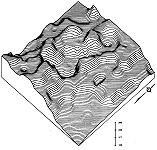
\includegraphics[width=.45\mycolumnwidth]{Historia/SYMVU.png}
\caption{\small Representaci�n tridimensional creada con SYMVU}
\label{Fig:SYMVU} 
\end{figure}

Si la d�cada de los sesenta es la de los pioneros y las primeras implementaciones, la de los setenta es la de la investigaci�n y el desarrollo. A partir de los SIG primitivos se va dando forma a un �rea de conocimiento sin duda con gran futuro, y se elabora una base s�lida de conocimiento y de herramientas aptas para un uso m�s gen�rico. Sin haber entrado a�n en la �poca del uso masivo y generalizado, los primeros paquetes comienzan a distribuirse y pasan a incorporarse a la comunidad cartogr�fica, lejos ya de ser el producto de unos pocos pioneros.

A partir de este punto, el campo de los SIG recorre sucesivas etapas hasta nuestros d�as (Figura \ref{Fig:Etapas_evolucion_SIG}), evolucionando muy r�pidamente ante la influencia de numerosos factores externos. Desde este punto, vamos a estudiar c�mo esos factores han ido a su vez evolucionando y c�mo su influencia ha condicionado el rumbo seguido por los SIG. Distinguiremos los siguientes elementos:

\begin{figure}[!hbt]   
\centering
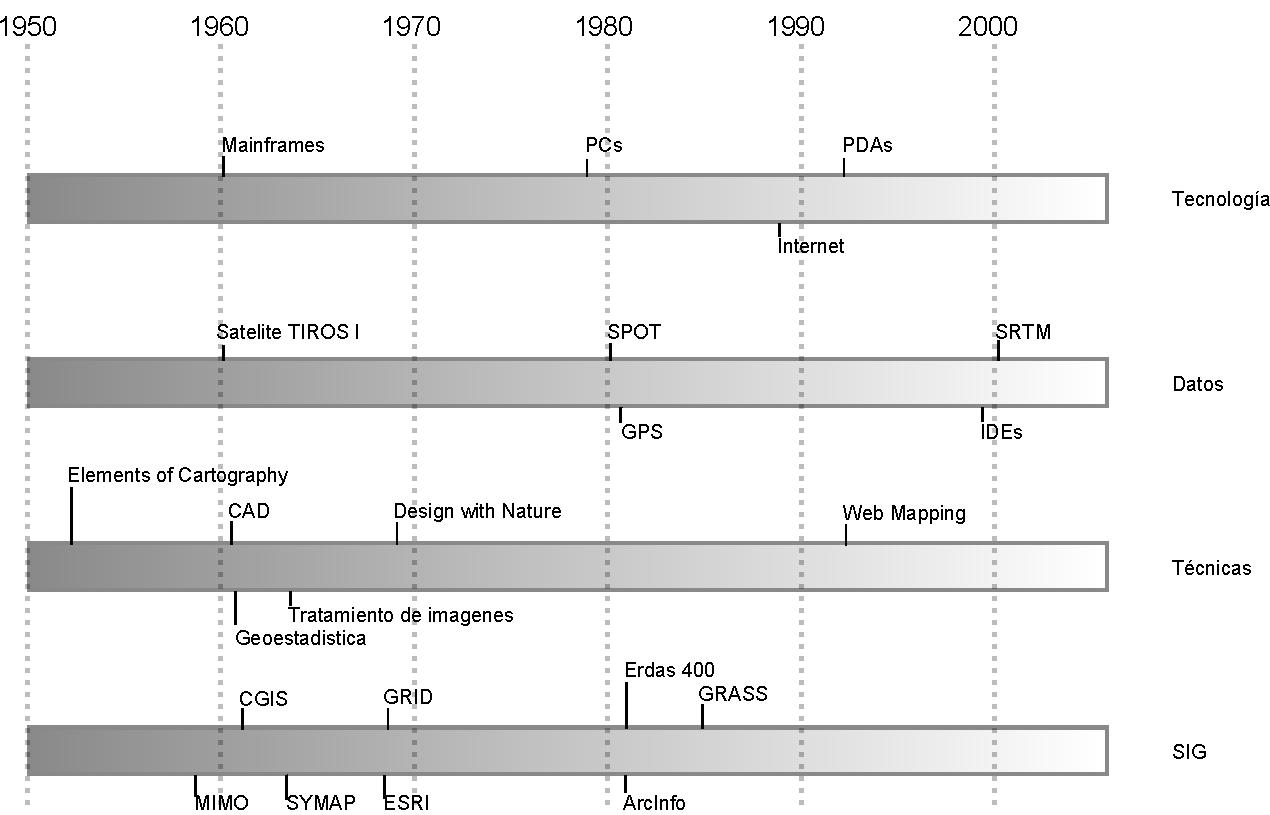
\includegraphics[width=.9\textwidth]{Historia/Etapas_historia.pdf}
\caption{\small Esquema temporal de la evoluci�n de los SIG.}
\label{Fig:Etapas_evolucion_SIG} 
\end{figure}

\begin{itemize}
\item La evoluci�n del SIG como disciplina. C�mo ha cambiado la presencia social de los SIG y su relaci�n con otras disciplinas cient�ficas, tanto influenci�ndolas como siendo influenciado por ellas.
\item La evoluci�n de la tecnolog�a. C�mo ha variado el \emph{software} SIG, as� como los ordenadores, perif�ricos y elementos inform�ticos de los que depende para su funcionamiento.
\item La evoluci�n de los datos. C�mo ha cambiado la generaci�n de datos, su almacenamiento, y c�mo esto ha condicionado el desarrollo de nuevas soluciones para su manejo.
\item La evoluci�n de las t�cnicas y formulaciones. Desde los elementos b�sicos de la cartograf�a cuantitativa, c�mo se han desarrollado nuevos conceptos, enfoques, teor�as o ramas de conocimiento de nueva aparici�n, que han dejado su huella en la evoluci�n de los SIG.
\end{itemize}

\section{La evoluci�n de los SIG como disciplina}

Como hemos visto, los SIG eran en origen una mera combinaci�n de elementos de cartograf�a cuantitativa, enlazados con los sistemas inform�ticos de la �poca. Se trataba de un territorio propio de cart�grafos y ge�grafos que intentaban adaptar sus conocimientos y necesidades a las tecnolog�as que por aquel entonces comenzaban a surgir. No obstante, desde aquellos or�genes los cambios han sido muy grandes, y se han incorporado al �mbito de los SIG un gran n�mero de otras disciplinas cuya aportaci�n e influencia puede ser equivalente o incluso superior a la de la cartograf�a o la geograf�a. 

La utilizaci�n del t�rmino <<geogr�fico>> para denominar a estos sistemas de manejo de informaci�n ha hecho que tradicionalmente, y a falta de una parcela de conocimiento propia bien delimitada, haya reca�do en la geograf�a la tarea docente e investigadora relacionada con los SIG. No obstante, y dada la multidisciplinaridad del �mbito y su uso por grupos muy distintos hoy en d�a, no es necesariamente este el mejor enfoque \cite{SarriaSIG}. En general, el conjunto de ciencias del medio y ciencias sociales han sabido todas ellas hacer uso de los SIG y aportar a estos los elementos propios de su �mbito.

Si bien los or�genes del SIG est�n �ntimamente ligados a la gesti�n forestal o la planificaci�n urban�stica, son muchas otras las disciplinas que han jugado un papel importante. Un elemento sin duda clave es la sensibilizaci�n medioambiental, que obliga a un estudio del medio mucho m�s detallado. Coincidiendo con la etapa inicial del desarrollo de los SIG, empieza a aparecer una preocupaci�n por el entorno que tiene consecuencias muy favorables para el desarrollo de todas las ciencias relacionadas, la gran mayor�a de las cuales son o ser�n usuarias directas de SIG. El SIG comienza a integrarse paulatinamente en las tareas de gesti�n del medio, como un apoyo imprescindible a la hora de analizar este.

Al principio de la d�cada de los setenta, siendo ya claro que los SIG son herramientas con gran futuro, aparecen no solo los esfuerzos de desarrollo y estabilizaci�n de la disciplina, sino todos los restantes que dan entidad propia a la prometedora ciencia de la informaci�n geogr�fica con base inform�tica.

As�, a finales de septiembre de 1970, apenas media d�cada despu�s de que el CGIS fuera desarrollado, tiene lugar en Ottawa, Canada, el primer Simposio Internacional de Sistemas de Informaci�n Geogr�fica. La celebraci�n de eventos similares ser� ya una actividad en constante aumento desde entonces.

Paralelamente, el SIG pasa a formar parte de los \emph{curricula} universitarios y a constituirse en una disciplina bien diferenciada, al tiempo que el mercado editorial comienza a prestar atenci�n a los SIG y aparecen obras cl�sicas que engloban toda la base conceptual de las herramientas modernas. Poco despu�s, se crean las principales revistas especializadas que recogen los avances y tendencias de una ciencia en muy r�pido desarrollo. 

En 1987 se empieza a publicar el \emph{International Journal Of Geographical Information Systems}\index{International Journal Of Geographical Information Systems}. Un a�o m�s tarde se funda en la Universidad Estatal de Nueva York, en Buffalo, la primera lista de distribuci�n en Internet dedicada a los SIG\index{Lista de distribuci�n}, y arranca la publicaci�n mensual \emph{GIS World}\index{GIS World}.

Los productos del Harvard Laboratory se hab�an vendido a precios m�dicos a otros investigadores para financiar su propio desarrollo, pero sin gran af�n comercial. La incorporaci�n de los SIG al mercado y la aparici�n de una industria basada en ellos aparece poco despu�s del inicio de estos, al final de los a�os sesenta. En 1969, Jack Dangermond\index{Dangermond, Jack}, un integrante del propio Harvard Laboratory, funda junto a su esposa la empresa Environmental Systems Research Institute (ESRI)\index{ESRI}\index{Environmental Systems Research Institute},  pionera y l�der del sector hasta el d�a de hoy. La popularizaci�n de los SIG y su conversi�n en un elemento de consumo es debida tambi�n en gran medida a la labor de ESRI dentro del mercado y a su l�nea original de productos.

Esta popularizaci�n de la herramienta, acompa�ada de la disponibilidad creciente de ordenadores personales, hace que los SIG pasen de ser elementos al alcance de unos pocos a estar disponibles para todos los investigadores en una gran variedad de �mbitos. La multidisciplinaridad de los SIG\index{SIG!multidisciplinaridad} como �tiles de trabajo para todas las ciencias del medio se ve reforzada a partir de este momento con continuas aportaciones por parte de estas y la aceptaci�n del SIG como un elemento m�s dentro de innumerables campos de trabajo.

Surgen nuevas empresas en el mercado, y en 1985 aparece el primer SIG libre, GRASS (Geographic Resources Analysis Support System)\index{GRASS}\index{Geographic Resources Analysis Support System}, siendo a�n en la actualidad el referente dentro de su �rea. Tambi�n en la d�cada de los 80, comienzan a perder sentido los primeros desarrollos con los que comenz� el SIG, y programas tales como CGIS no se encuentran ya en condiciones de competir en el mercado, que se desarrolla muy r�pidamente y va creando soluciones adaptables.

En este sentido, es rese�able el hecho de que los SIG dejan de ser sistemas completos y pasan a ser plataformas adaptables sobre las que construir soluciones particulares. Los SIG se convierten en herramientas base para todo ese gran conjunto de disciplinas beneficiarias, cada una de las cuales adapta y particulariza estos a la medida de sus necesidades.

Con el paso del tiempo, los SIG van confluyendo y los diversos enfoques se unen para constituir una base �til sobre la que construir nuevos desarrollos. Los SIG r�ster incluyen cada vez m�s elementos vectoriales, los SIG vectoriales cada vez m�s elementos r�ster, y en ambos se van implementando formulaciones que trabajan con ambos formatos de almacenamiento y los combinan. De forma similar, los procesos para an�lisis de im�genes van ganando su espacio dentro de los SIG generales, aunque no dejan de existir aplicaciones espec�ficas en este terreno.

Por �ltimo, respecto a su presencia social, en nuestros d�as los SIG han pasado de elementos restringidos para un uso profesional a ser elementos de consumo y estar presentes en nuestra vida diaria. Un ejemplo de ello es la aparici�n de servicios como \emph{Google Maps}\index{Google!Maps}\cite{webGoogleMaps} y la multitud de aplicaciones con interfaces Web basadas en �l que permiten acceder a informaci�n geogr�fica de toda clase. De la mano tambi�n de \emph{Google}, \emph{Google Earth}\index{Google!Earth}\cite{webGoogleEarth} es otra aplicaci�n popular que no est� restringida al uso profesional.  Estas aplicaciones acercan los SIG a usuarios no especializados, d�ndoles la posibilidad de utilizarlos y aprovechar parte de sus capacidades. 

La popularizaci�n de los navegadores GPS, que incorporan tanto elementos de representaci�n como de an�lisis propios de los SIG, son otro buen ejemplo.

\section{La evoluci�n de la tecnolog�a}

La tecnolog�a sobre la que se basan los SIG es clave para entender todo lo relacionado con ellos, especialmente su evoluci�n a lo largo del tiempo. Desde los primeros SIG muy lejos del alcance de un usuario medio, hasta las aplicaciones de escritorio o los elementos derivados de los SIG que son de uso habitual hoy en d�a, se ha producido un cambio enorme que, como cabe esperar, es paralelo al que la propia tecnolog�a ha sufrido.

Tres son los bloques principales del desarrollo inform�tico con una influencia m�s marcada en el campo de los Sistemas de Informaci�n Geogr�fica \cite{Heywood1998Longman}:

\begin{itemize}
 \item Salidas gr�ficas. Sin las capacidades de representaci�n gr�ficas de hoy en d�a, puede parecernos imposible el uso de un SIG, ya que, aunque los procesos de an�lisis son una parte imprescindible y definitoria del mismo y pueden llevarse a cabo sin necesidad de visualizaci�n, esta visualizaci�n es una herramienta fundamental de un SIG. No obstante, tanto los primeros ordenadores como las primeras impresoras dedicadas a la impresi�n de mapas  carec�an de dichas capacidades. Como puede verse en la figura \ref{Fig:SYMAP}, las representaciones en esos tiempos se basaban en el uso de caracteres y no en gr�ficos puramente dichos.

La evoluci�n de las capacidades gr�ficas, intensa desde esos inicios hasta nuestros d�as y a�n muy activa, ha sido seguida de cerca por los SIG, que progresivamente van incorporando mejoras tanto en la representaci�n en pantalla como en la generaci�n de mapas impresos.
\item Almacenamiento y acceso de datos. Desde el inicio, el almacenamiento y acceso de datos ha sido un problema clave en el cual se han producido grandes avances. Por una parte, los problemas asociados a los grandes vol�menes de informaci�n. Por otra, los relacionados con la lectura de estos, que ha de realizarse de forma fluida pese a dicho volumen. A medida que han ido aumentando las capacidades de almacenamiento y lectura, ha ido aumentando paralelamente el tama�o de los datos manejados, as� como los soportes utilizados para ellos, y esta evoluci�n paralela ha de continuar y condicionar la forma que adopten los SIG.
\item Entrada de datos. Los datos geogr�ficos utilizados en los primeros a�os de los SIG eran datos en papel que se digitalizaban y almacenaban mec�nicamente en tarjetas perforadas en un �nico proceso mec�nico. Hoy en d�a, y aunque veremos que las fuentes de datos han sufrido por su parte una gran evoluci�n, sigue siendo necesaria la digitalizaci�n de una gran cantidad de datos. Desde esos sistemas mec�nicos de tarjetas hasta los modernos equipos, la aparici�n de \emph{scanners}\index{Scanner} de gran precisi�n y t�cnicas de digitalizaci�n autom�ticas, entre otros, ha cambiado completamente el �mbito de la entrada de datos para su uso en un SIG.
\end{itemize}

Adem�s del avance de estos factores, la evoluci�n general de los ordenadores afecta a todos los elementos de \emph{software} que se ejecutan sobre ellos. De las grandes computadoras se pasa a los ordenadores personales, y los programas tales como los SIG realizan tambi�n esa transici�n de una a otra plataforma.

La elaboraci�n y an�lisis de cartograf�a se convierte a finales de los a�os 80 en una tarea que puede ya llevarse a cabo en equipos personales (PC) de bajo coste, lejos de las grandes m�quinas y equipos dedicados de alto coste.

En 1978, la recientemente creada empresa ERDAS\index{ERDAS} adapta para el PC un \emph{software} de an�lisis de im�genes denominado IMGGRID\index{IMGGRID}, y comienza a distribuir este junto con un hardware relativamente asequible para uso personal. El ERDAS 400 System se convierte as� en el primero de su clase con esas caracter�sticas.

Paralelamente, ArcInfo\index{ArcInfo}, de la compa��a ESRI, se convierte en 1981 en el primer SIG que alcanza el �mbito de los ordenadores personales. Ser� tambi�n un producto de esta compa��a, ArcView\index{ArcView}, el que en 1991 pase a popularizar el SIG como herramienta de escritorio.

A mitad de los 80, ArcInfo y ERDAS comienzan a distribuirse de forma conjunta en un producto comercial que integra el an�lisis vectorial con el tratamiento de im�genes dentro del entorno de un PC.

La evoluci�n de las plataformas no se detiene ah�. Las tendencias actuales apuntan a llevar los SIG de forma gen�rica a plataformas m�viles tales como PDA, especialmente indicadas para la toma de datos en campo. La combinaci�n de PDA y GPS se demuestra altamente pr�ctica en este aspecto.

Elementos de SIG se incluyen tambi�n en los navegadores GPS cada d�a m�s populares, confirmando la tendencia de adaptar los SIG a los dispositivos port�tiles, tanto para el an�lisis como para la consulta de la informaci�n geogr�fica.

La aparici�n de Internet es un hecho que ha modificado todos los aspectos de la sociedad actual, est�n relacionados o no con �mbito cient�fico. Los SIG no son, como cabe esperar, una excepci�n a esto, e Internet ha jugado un papel decisivo en redefinir el concepto de SIG que hoy conocemos.

El nacimiento de la World Wide Web (WWW) puede establecerse a finales de 1989, pero no ser� hasta 1993 cuando empiece a utilizarse directamente para actividades relacionadas con los SIG o la distribuci�n de cartograf�a. En esta fecha aparece \emph{Xerox PARC}\index{Xerox PARC}, el primer servidor de mapas. \emph{Mapserver}\index{Mapserver}, uno de los principales servidores de cartograf�a en la actualidad, aparece a mediados de 1997.

El primer atlas digital en linea es el Atlas Nacional de Canad�, que se encuentra disponible desde 1994. Otros como MultiMap\index{MultiMap} o MapQuest\index{MapQuest}, que alcanzan gran popularidad, aparecen en 1996 y establecen la l�nea a seguir por otros servicios de Internet relacionados con la informaci�n geogr�fica.

En 2005 aparece Google Maps\cite{webGoogleMaps}\index{Google!Maps}, que adem�s de ofrecer servicios de cartograf�a permite desarrollar nuevas aplicaciones sobre dichos servicios a trav�s de una interfaz de programaci�n abierta y documentada. Los conceptos de la Web 2.0\index{Web 2.0} se adaptan as� al �mbito de los SIG. El n�mero de ideas y funcionalidades basados en Google Maps crece exponencialmente desde pr�cticamente su nacimiento, extendiendo la tecnolog�a SIG a campos casi insospechados y muy distintos de los que originalmente constitu�an el �mbito de uso de los SIG.

\section{La evoluci�n de los datos}

Los datos son el elemento principal del trabajo dentro de un SIG. Sin ellos, no tiene sentido un Sistema de Informaci�n Geogr�fica. Esta relaci�n entre los datos y los elementos de \emph{software} y \emph{hardware} empleados en su manejo ha ejercido una notable influencia en el desarrollo de las tecnolog�as SIG y, rec�procamente, estas han definido el marco de trabajo para los avances en los tipos de datos. 

En los or�genes, los primeros SIGs dieron soluci�n al problema de la codificaci�n de datos, e intentaron adaptar la cartograf�a disponible. Los primeros datos geogr�ficos con los que se trabajaba proven�an de la digitalizaci�n de cartograf�a impresa. La primeras bases de datos geogr�ficas conten�an mapas escaneados y elementos digitalizados en base a estos.

A partir de este punto, no obstante, van apareciendo nuevas fuentes de datos cuya estructura es m�s adecuada para su tratamiento informatizado, y al tiempo que los SIG se adaptan a estas, surge una relaci�n bidireccional que resulta beneficiosa para ambos.

Un avance primordial en este sentido lo constituye el lanzamiento de los primeros sat�lites de observaci�n terrestre. Las t�cnicas existentes para la toma de fotograf�as a�reas, desarrolladas principalmente con fines militares durante la Primera Guerra Mundial, pasan a ser aplicadas a escala global con la aparici�n de sat�lites destinados a estos efectos. 

El 1960, el primer sat�lite de observaci�n meteorol�gico, el \emph{TIROS I}\index{TIROS I}, es lanzado al espacio. Dos a�os despu�s, Rusia lanza su sat�lite \emph{Kosmos}\index{Kosmos}, y en 1974 el primer prototipo del sat�lite SMS--1\index{SMS--1} es puesto en �rbita.

Otros hitos importantes son los lanzamientos de los sat�lites LANDSAT\index{LANDSAT} 2 y 7 en 1975 y 1999 respectivamente, cuyos productos son ambos de uso muy extendido (como veremos en el cap�tulo \ref{Fuentes_datos}).

El 1980 se funda SPOT\index{SPOT}, la primera compa��a mundial en ofrecer con car�cter comercial im�genes procedentes de sat�lite para toda la superficie terrestre. A este hecho le seguir�a el lanzamiento de un buen n�mero de nuevos sat�lites con o sin fines comerciales. Los productos de la teledetecci�n pasan a constituir una fuente de negocio, al tiempo que se incorporan como elementos b�sicos del an�lisis geogr�fico.

Las tecnolog�as de posicionamiento y localizaci�n son otra fuente de datos de primer orden. En 1981, el sistema GPS\index{GPS} pasa a ser plenamente operativo, y en 2000 se ampl�a la precisi�n de este para uso civil. Este �ltimo hecho aumenta la penetraci�n de la tecnolog�a, pudiendo ya ser empleado el sistema para el desarrollo de elementos como navegadores GPS u otros productos derivados, hoy en d�a de uso com�n.

Al igual que las aplicaciones, los distintos tipos de datos geogr�ficos digitales se van asentando y popularizando, recibiendo progresivamente m�s atenci�n y medios. El Servicio Geogr�fico Estadounidense (USGS)\index{USGS} publica en 1976 los primeros Modelos Digitales de Elevaciones (MDE), en respuesta a la gran importancia que este tipo de dato tiene dentro del nuevo contexto del an�lisis geogr�fico. 

La evoluci�n de los datos de elevaci�n  a nivel global llega a un punto hist�rico en el a�o 2000 con la \emph{Shuttle Radar Topographic Mission}\index{SRTM}\index{Shuttle Radar Topographic Mission} (SRTM). La SRTM es un proyecto conjunto dirigido entre la NASA\index{NASA} y la National Imagery and Mapping Agency\index{National Imagery and Mapping Agency} (NIMA)\index{NIMA}, cuyo objetivo es ofrecer informaci�n altitudinal de un 80\% de la superficie terrestre a una resolucion de un segundo de arco (aproximadamente, 30 metros).

La aparici�n de nuevas t�cnicas tales como el LiDAR (ver \ref{Sensores})\index{LiDAR} abre nuevos caminos en cuanto a la precisi�n que puede obtenerse en la caracterizaci�n del terreno, posibilitando nuevos usos y an�lisis antes no planteados.

La evoluci�n de los datos no es solo una evoluci�n t�cnica, sino tambi�n de car�cter social y organizativo. En la denominada \emph{era de la informaci�n}, el papel de los datos es tenido cada vez m�s en cuenta, y los esfuerzos para coordinar la enorme cantidad de datos espaciales y sus numerosas procedencias se hacen cada vez m�s relevantes. Se empieza a entender que resulta necesario formular estrategias adecuadas para la gesti�n de los datos espaciales. Estas estrategias pasan por la creaci�n de las denominadas \emph{Infraestructuras de Datos Espaciales} (IDE)\index{Infraestructuras de Datos Espaciales}\index{IDE}, a las cuales se dedica una cap�tulo completo de este libro.

El ejemplo m�s destacado de estas es la IDE Nacional de los Estados Unidos (NSDI)\index{NSDI}\cite{Clinton1994FR}, surgida a ra�z de la Orden Ejecutiva 12096, que fue promulgada en 1994 y tuvo una vital importancia en este �mbito. En Europa, la directiva INSPIRE\cite{Craglia2009INSPIRE}, con fecha 14 de marzo de 2007, pretende la creaci�n de una infraestructura similar.

Muchos de estos desarrollos y actividades se adhieren a las especificaciones establecidas por el \emph{Open GIS Consortium}\index{Open GIS Consortium}\index{OGC} (OGC), un consorcio internacional fundado en 1994 para homogeneizar el empleo y difusi�n de los datos geogr�ficos.

\section{La evoluci�n de las t�cnicas y formulaciones}\label{Evolucion_tecnicas}

Los problemas iniciales de los pioneros del SIG eran el desarrollo de los primeros programas --- esto es, la mera implementaci�n --- y los relativos al almacenamiento y codificaci�n de datos, como ya vimos. Las formulaciones de estos inicios eran las de la cartograf�a cuantitativa del momento, a�n no muy desarrollada. Una vez que se implementan los primeros SIG y se suplen las necesidades de an�lisis y gesti�n de datos espaciales que motivaron su aparici�n, comienza el proceso de desarrollar nuevas t�cnicas y planteamientos que permiten ir m�s all� en dicho an�lisis. 

La cartograf�a cuantitativa sufre desde entonces un avance muy notable, arrastrada por las necesidades de los SIG en su propia evoluci�n, y muchas disciplinas cient�ficas desarrollan nuevas formulaciones que comienzan a tener como base los Sistemas de Informaci�n Geogr�fica. Algunas de ellas resultan especialmente relevantes y pasan a formar parte del conjunto habitual de herramientas y elementos de un SIG gen�rico.

Como indica \cite{Martin1991Routledge} la mayor�a de los avances de cierta importancia dentro del mundo de los SIG han venido motivadas por las necesidad de una utilizaci�n concreta o por la tecnolog�a en s�, y pocas veces por el desarrollo puro de una teor�a. No obstante, e independientemente de las razones que lo motiven, los SIG han servido como contexto ideal para dar cuerpo a estas teor�as, y su historia debe considerarse de forma pareja.

Antes de que aparecieran los primeros SIG, los trabajos de algunos pioneros establecen bases que m�s tarde ser�n de gran importancia para otros avances. Junto con el ya citado \emph{Elements of Cartography} de John K.Wright, los trabajos de Ian McHarg\index{McHarg, Ian} anticipan una forma de operar con los datos geogr�ficos que m�s adelante va a convertirse en una constante del trabajo con estos dentro de un SIG. En su libro \emph{Design with Nature}\index{Design with Nature} (1969), McHarg define los elementos b�sicos de la superposici�n y combinaci�n de mapas, que, como veremos m�s adelante, son los que se aplican tanto en el an�lisis como en la visualizaci�n de las distintas \emph{capas} de datos geogr�ficos en un SIG.

Aplicaciones de esta �ndole, en las cuales se combinan diversos mapas tem�ticos, ya se hab�an llevado a cabo con anterioridad. McHarg, sin embargo, es el encargado de generalizarlas como metodolog�as de estudio y an�lisis geogr�fico, asentando as� los fundamentos que luego se introducir�n dentro de los SIG.

El trabajo de McHarg tiene, adem�s, un fuerte componente medioambiental, elemento que, como ya se ha dicho, es una de las razones que impulsan al desarrollo de los SIG como herramientas para una mejor gesti�n del medio.

Antes de McHarg, ya se hab�an empezado a realizar an�lisis cartogr�ficos, arrancando la l�nea que llega hasta los procedimientos que actualmente empleamos en un SIG. M�s de cien a�os antes, John Snow (1813--1858)\index{Snow, John} realiz� la que puede considerarse como una de las primeras experiencias cartogr�ficas anal�ticas, al utilizar mapas de puntos para efectuar sus deducciones y localizar en Inglaterra la fuente de un brote de c�lera.

Junto con la componente anal�tica, otros elementos de la pr�ctica cartogr�fica evolucionan similarmente. En 1819, Pierre Charles Dupin crea el primer mapa de coropletas\index{Mapa!de coropletas}\index{Dupin, Pierre Charles} para mostrar la distribuci�n del analfabetismo en Francia, dando un gran salto cualitativo en el dise�o cartogr�fico, particularmente en un tipo de mapas de muy habitual creaci�n dentro de un SIG.

Una vez que los SIG ya han hecho su aparici�n, entre los elementos que m�s han impulsado el desarrollo de estos cabe destacar el gran avance en el estudio del relieve, de notable importancia por ser un elemento base para muchos otros an�lisis en un amplio abanico de ciencias afines. La orograf�a cl�sica, con un enfoque tradicionalmente sustentado en la geolog�a y el an�lisis geomorfol�gico, va dando lugar a una ciencia cada vez m�s cuantitativa centrada en el an�lisis morfom�trico del relieve. Trabajos como los de \cite{Evans1972Harper} sientan las bases para este tipo de an�lisis, que necesitan de un SIG para ser aplicados de forma efectiva.

De igual modo sucede con la geoestad�stica\index{Geoestad�stica}, una rama de la estad�stica que aparece de la mano del franc�s Georges Matheron\index{Matheron, George} a principio de los a�os sesenta. Las formulaciones geoestad�sticas, hoy parte caracter�stica de los SIG, son desarrolladas en esa �poca desde el punto de vista te�rico, aunque no son aplicables para un uso real si no es con el uso de ordenadores, y pierden gran parte de su valor pr�ctico si no se realiza esta tarea con el concurso de Sistemas de Informaci�n Geogr�fica.

En general, el desarrollo de la estad�stica encaminado a la adaptaci�n de teor�as y metodolog�as al �mbito espacial ha tenido un fuerte crecimiento en las �ltimas d�cadas, un hecho muy ligado a la aparici�n y evoluci�n de los SIG. Uno de los hitos de este proceso es el desarrollo de \cite{Whittle1954Biometrika}, que extiende los modelos autoregresivos\index{Modelos!autoregresivos}, de importancia clave para el an�lisis de la variaci�n de series temporales, a los datos espaciales \cite{Goodchild2003JoE}.

El desarrollo de otras ramas de conocimiento ha sido igualmente clave para el enriquecimiento de la ciencia del an�lisis geogr�fico. Muchas de ellas, por depender tambi�n en gran medida de la componente inform�tica, ha evolucionado paralelamente a los SIG, pues el desarrollo de las tecnolog�as ha jugado un papel similar en ellas.

Otro hecho importante es la aparici�n de los primeros programa de dise�o asistido por ordenador (CAD) \index{CAD}\index{Dise�o!Asistido por Ordenador|see{CAD}}, que coincide con la de los SIG, all� por el final de los a�os sesenta. Originalmente pensados para el dise�o industrial, pronto pasan a ser utilizados para el dise�o arquitect�nico y la delineaci�n de elementos geogr�ficos, y sus conceptos son incorporados paulatinamente a los SIG. Hoy en d�a, y cada vez con m�s frecuencia, los SIG  incorporan capacidades similares a los sistemas CAD, que permiten tanto la digitalizaci�n de cartograf�a con las herramientas propias del CAD como la creaci�n de nuevos elementos geogr�ficos. Asimismo, los formatos habituales de las aplicaciones CAD son soportados por gran n�mero de SIG, existiendo una cierta interoperabilidad\index{Interoperatividad}, no obstante muy mejorable. Firmas como Autodesk\index{Autodesk} tienen presencia en el mercado tanto del SIG como del CAD, compaginando ambas y compartiendo parcialmente soluciones y elementos.

El avance en el desarrollo de las aplicaciones CAD, y en general de las representaciones gr�ficas por ordenador, impuls� igualmente la aparici�n y evoluci�n posterior de una nueva disciplina: la geometr�a computacional\index{Geometr�a computacional}. Esta denominaci�n se emplea por primera vez en 1975 \cite{Preparata1985Springer}, siendo hoy el nombre de una rama de la ciencia consolidada y en constante avance. Los algoritmos que componen la geometr�a computacional son la base sobre la que se fundamenta el an�lisis vectorial dentro de un SIG.

\section{Resumen}

A principios de los a�os sesenta, el creciente inter�s por la informaci�n geogr�fica y el estudio del medio, as� como el nacimiento de la era inform�tica, propiciaron la aparici�n de los primeros SIG.

Desde ese punto hasta nuestros d�as, los SIG han ido defini�ndose en base a la evoluci�n de la inform�tica, la aparici�n de nuevas fuentes de datos susceptibles de ser utilizadas en el an�lisis geogr�fico --- muy especialmente las derivadas de sat�lites ---, y del desarrollo de disciplinas relacionadas que han contribuido a impulsar el desarrollo propio de los SIG.

Siendo en su origen aplicaciones muy espec�ficas, en nuestros d�as los SIG son aplicaciones gen�ricas formadas por diversos elementos, cuya tendencia actual es a la convergencia en productos m�s vers�tiles y amplios.

%\bibliographystyle{unsrt}
%\bibliography{../../Libro_SIG}


\chapter{Fundamentos cartogr�ficos y geod�sicos}\label{Fundamentos_cartograficos}

\begin{keypoints}
�Qu� aspectos trata la geodesia y por qu� es necesario conocer estos para trabajar con un SIG? $\bullet$ �Qu� es el geoide? $\bullet$ �Qu� es el datum? $\bullet$ �Qu� es un sistema de proyecci�n y cu�les son los principales? $\bullet$ �Qu� diferencias existen entre ellos? $\bullet$  �Qu� es la escala?  $\bullet$ �Qu� entendemos por generalizaci�n cartogr�fica y para qu� resulta �til?
\end{keypoints}

\bigskip

\begin{intro}
Trabajar con informaci�n georreferenciada requiere conocer una serie de conceptos previos necesarios para poder realizar correctamente todo tipo de operaciones. Estos conceptos no son exclusivos del �mbito de los SIG, sino que derivan de otras disciplinas que tradicionalmente han trabajado con este tipo de informaci�n, como por el ejemplo la cartograf�a.

Los datos georreferenciados tienen adem�s una peculiaridad como datos espaciales, pues son datos que se sit�an sobre la superficie de la Tierra. Por ello, es necesario tener un conocimiento preciso de la forma de esta, para as� tratar con exactitud y rigor la informaci�n con que se trabaja en un SIG. La geodesia es la ciencia que se encarga del estudio de la forma de la Tierra, y sus fundamentos se encuentran entre los conceptos base de todo SIG, siendo por tanto necesario conocerlos para poder hacer uso de estos.

En este cap�tulo veremos algunas ideas esenciales sobre cartograf�a y geodesia, que ser�n de aplicaci�n constante y fundamental en el uso de cualquier SIG.
\end{intro}

\section{Introducci�n}

La caracter�stica principal de la informaci�n georreferenciada es que tiene una localizaci�n en el espacio, particularmente en el espacio terrestre. Esta localizaci�n se ha de dar por medio de unas coordenadas que la definan de forma adecuada, lo cual implica la necesidad de establecer un sistema en base al cual expresar dichas coordenadas. 

Si medimos un dato de temperatura necesitamos un sistema de medici�n conocido, sin el cual el dato de temperatura en s� carece de valor y significado. As�, no es lo mismo decir que una temperatura es de 25 grados Celsius o que es de 25 grados Fahrenheit. Del mismo modo, si a esa temperatura le queremos asociar alg�n tipo de informaci�n espacial (por ejemplo, el punto exacto en el que fue medida), debemos establecer un sistema que permita dar sentido a las mediciones que realicemos, y que posteriormente nos sirva para interpretar los valores de las coordenadas y poder saber con exactitud \emph{d�nde} est� el punto al que estas hacen referencia.

El establecimiento de un sistema de referencia en el que expresar la situaci�n de un punto dado no es en absoluto una tarea sencilla, y requiere el conocimiento de abundantes conceptos previos que van desde ideas f�sicas hasta complejos desarrollos matem�ticos y geom�tricos. Los avances en este campo han sido constantes desde la antig�edad, y esta evoluci�n es la que ha permitido que en la actualidad se puedan obtener resultados altamente precisos en el trabajo con informaci�n georreferenciada. Gran parte de lo que podemos hacer en un SIG carecer�a de sentido si no se dispusiera de metodolog�as bien desarrolladas para el establecimiento de sistemas de referencia.

La geodesia es la ciencia encargada de proveer el marco te�rico en el que fundamentar todo lo anterior, y es una disciplina compleja con diversas ramas de estudio. Todas ellas responden al objetivo b�sico de estudiar la forma de la Tierra, ya que debemos saber c�mo es la Tierra para poder localizar puntos sobre su superficie. La determinaci�n de la forma y dimensiones de la Tierra es tarea de la denominada \emph{geodesia esferoidal}\index{Geodesia!esferoidal}, cuyo cometido coincide con el del concepto cl�sico de geodesia, esto es, la definici�n de la figura terrestre. No obstante, en la actualidad encontramos otras ramas como la \emph{geodesia f�sica}\index{Geodesia!f�sica}, encargada de analizar el campo gravitatorio terrestre y sus variaciones, o la \emph{astronom�a geod�sica}\index{Astronom�a geod�sica}, que utiliza m�todos astron�micos para la determinaci�n de ciertos elementos geod�sicos muy importantes que veremos m�s adelante. En conjunto, todas estas ramas dan forma a una serie de m�todos y conceptos que son los que van a permitir  la utilizaci�n rigurosa de coordenadas.

La necesidad del estudio geod�sico surge por el hecho de que la Tierra no es plana, y cuando el territorio que pretendemos estudiar es lo suficientemente extenso, la curvatura de la Tierra no puede ser ignorada. Este es el caso que vamos a encontrar cuando trabajemos con un SIG, y es por ello que los SIG implementan los elementos necesarios para poder efectuar un manejo de la informaci�n geogr�fica riguroso y acorde con los conceptos de la geodesia.

Vimos en el primer cap�tulo de esta parte que existen otras aplicaciones que trabajan con informaci�n georreferenciada, entre las cuales estaban los programas de dise�o asistido por ordenador (CAD)\index{CAD}. Dec�amos entonces que una de las principales limitaciones de estos era su mala disposici�n al trabajo con zonas extensas, ya que han sido dise�ados para operar con zonas de unas dimensiones reducidas. 

Cuando un arquitecto dise�a el plano de una casa con una aplicaci�n CAD, no necesita emplear los conceptos de la geodesia, puesto que a esa escala la forma de la Tierra no tiene relevancia, y prescindiendo de ella puede expresar las coordenadas de los distintos elementos (un muro, un pilar, etc.) con la suficiente precisi�n y correcci�n como para que luego pueda construirse esa casa.  Sin embargo, cuando un usuario de SIG estudia la cuenca vertiente de un r�o o la distribuci�n de poblaci�n en las comunidades aut�nomas de un pa�s, o bien analiza las rutas migratorias de un ave entre dos continentes, los conceptos de la geodesia resultan fundamentales. 

En la actualidad, los SIG han hecho que la informaci�n geogr�fica tenga en muchos casos car�cter global y cubra grandes extensiones o incluso la totalidad del planeta. Esto obliga m�s que nunca a hacer hincapi� en los fundamentos geod�sicos que resultan b�sicos para que toda esa informaci�n pueda manejarse correctamente, siendo de inter�s para cualquier usuario de SIG, con independencia de su escala de trabajo.

Otro aspecto b�sico a la hora de trabajar en un SIG son las denominadas \emph{proyecciones cartogr�ficas}\index{Proyecci�n}. Estas permiten transformar las coordenadas sobre la superficie curva de la Tierra en coordenadas sobre una superficie plana. Esto es necesario para poder representarlas en un soporte plano tal como puede ser un mapa o la pantalla del ordenador, as� como para poder analizarlas de forma m�s simple.

Con los elementos de la geodesia y las proyecciones cartogr�ficas ya podemos elaborar cartograf�a y estamos en condiciones de trabajar con la informaci�n georreferenciada. No obstante, existen ciertos conceptos relativos a esa cartograf�a que resultan de suma importancia y deben conocerse antes de abordar esas tareas. El m�s importante de ellos es la escala\index{Escala}, es decir, la relaci�n entre el tama�o real de aquello que representamos y su tama�o en la representaci�n, la cual constituye un factor b�sico de toda informaci�n cartogr�fica. 

La escala condiciona a su vez la aparici�n de otra serie de ideas y de procesos asociados, como por ejemplo la generalizaci�n cartogr�fica\index{Generalizaci�n!cartogr�fica}. Esta engloba los procedimientos que permiten que a cada escala se represente la informaci�n de la forma m�s adecuada posible, maximizando el valor de dichas representaciones. Aunque tanto la escala como la generalizaci�n cartogr�fica son conceptos muy vinculados a las propias representaciones visuales de la informaci�n geogr�fica, y este libro contiene una parte dedicada espec�ficamente a la visualizaci�n, se trata de conceptos cartogr�ficos fundamentales y por ello se incluyen en este cap�tulo, ya que resultan necesarios incluso si se trabaja con datos georreferenciados sin visualizaci�n alguna de estos.

\section{Conceptos geod�sicos b�sicos}

A la hora de definir la forma y dimensiones de la Tierra, la geodesia plantea modelos que puedan recoger la complejidad natural de la superficie terrestre y expresarla de una forma m�s simple y f�cil de manejar. 

Con estos modelos, uno de los objetivos principales de la geodesia es establecer un sistema de referencia y definir un conjunto de puntos (conocidos como \emph{v�rtices geod�sicos})\index{V�rtice geod�sico} cuyas coordenadas en dicho sistema sean conocidas con una precisi�n elevada. Posteriormente, y en base a esos puntos, los cuales forman una \emph{red geod�sica}\index{Red geod�sica}, se pueden calcular las coordenadas de cualquier punto en el sistema de referencia definido.

Los v�rtices geod�sicos se establecen por triangulaci�n a partir de un punto �nico determinado por m�todos astron�micos. En funci�n de la longitud de los lados de los tri�ngulos empleados en dicha triangulaci�n, tenemos redes de mayor o menor precisi�n.

Veamos ahora c�mo establecer los elementos necesarios para establecer ese sistema de referencia base y definir esos modelos de partida citados. A la hora de buscar un modelo al que asimilar la forma de la Tierra, existen dos conceptos b�sicos: el  \emph{elipsoide de referencia} y el \emph{geoide}.

\subsection{Elipsoide de referencia y geoide}

\index{Elipsoide!de referencia}\index{Geoide}
El intento m�s b�sico de establecer un modelo de la forma de la Tierra es asimilar esta a una figura geom�trica simple, la cual pueda expresarse mediante una ecuaci�n matem�tica. Adem�s de ser m�s sencilla de manejar, disponer de esta ecuaci�n matem�tica permite la aplicaci�n de conceptos geom�tricos, estableciendo as� una base pr�ctica para el trabajo con coordenadas y la definici�n de sistemas de referencia.

Desde la antig�edad, se han formulado numerosas hip�tesis sobre la forma que la Tierra ten�a, las cuales van desde suponer la Tierra plana a admitir la evidencia de que esta ha de tener forma esf�rica (o similar) si se atiende a diversos hechos como, por ejemplo, el movimiento circular de las estrellas o la existencia de horizonte.

En realidad, la Tierra no es una esfera perfecta, ya que su propia rotaci�n ha modificado esa forma y ha provocado un achatamiento en los polos. Esta hip�tesis fue ya planteada por Newton\index{Newton, Isaac}, y corroborada posteriormente con numerosas experiencias. No obstante, podemos seguir tratando de asimilar la forma de la Tierra a la de una superficie te�rica, aunque no ya la de una esfera sino la de lo que se denomina un \emph{elipsoide}. Sobre un elipsoide, el radio de la Tierra ya no es constante, sino que depende del emplazamiento.

Suponer que la Tierra es una esfera no es una aproximaci�n tan mala como puede parecer (las representaciones gr�ficas a las que estamos acostumbrados exageran habitualmente mucho el achatamiento del planeta), aunque el elipsoide es m�s preciso y necesario a la hora de elaborar cartograf�a de zonas no muy extensas. A gran escala, sin embargo, y para determinadas tareas, es habitual suponer la Tierra con una forma perfectamente esf�rica.

Como se muestra en la figura \ref{Fig:Elipsoide}, un elipsoide viene definido por dos par�metros: el semieje mayor\index{Semieje!mayor}\index{Semieje!menor} y el semieje menor. En el caso de la Tierra estos se corresponder�an con el radio ecuatorial y el radio polar respectivamente. La relaci�n existente entre estas dos medidas define el grado de achatamiento del elipsoide. En particular, se establece un factor de achatamiento seg�n 

\begin{equation}
f=\frac{r_1-r_2}{r_1}
\end{equation}

\noindent siendo $r_1$ el semieje mayor y $r_2$ el semieje menor.

\begin{figure}
\centering
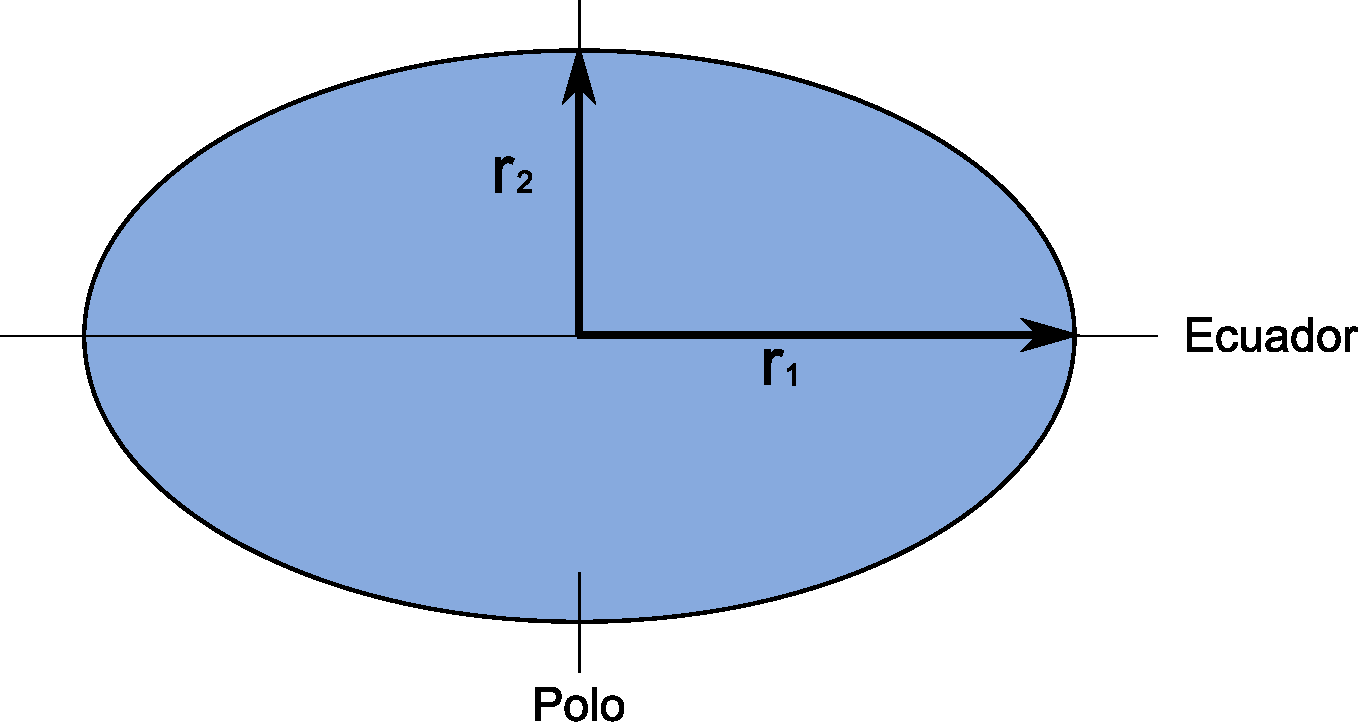
\includegraphics[width=.6\mycolumnwidth]{Fundamentos_cartograficos/Elipsoide.pdf}
\caption{\small Par�metros que definen el elipsoide}
\label{Fig:Elipsoide} 
\end{figure}

El elipsoide es la forma geom�trica que mejor se adapta a la forma real de la Tierra, y por tanto la que mejor permite idealizar esta, logrando un mayor ajuste. \index{Elipsoide}

Una vez que se dispone de una expresi�n te�rica para la forma de la Tierra, el siguiente paso es la determinaci�n de los par�metros que definen esta. En el caso de utilizar la esfera, hay que calcular su radio. En el caso de asumir el elipsoide como forma de referencia, deben determinarse las medidas de los semiejes menor y mayor. 

Debido a la evoluci�n hist�rica de la idea de elipsoide de referencia, las medidas de los semiejes que lo definen no son �nicas. Es decir, no en todos lugares y en todas las circunstancias se emplea un mismo elipsoide caracterizado por unos valores $r_1$ y $r_2$ id�nticos. Esto es debido principalmente al hecho de que un determinado elipsoide no se adapta de modo igualmente preciso a todas las regiones terrestres, y el elipsoide que proporciona un mejor ajuste para un �rea dada (por ejemplo, un continente o pa�s) puede no ser el mejor en otra zona de la Tierra alejada de la primera. 

A esto debe sumarse que los esfuerzos iniciales por determinar la forma de la Tierra y los par�metros del elipsoide de referencia fueron realizados en tiempos en los que la comunicaci�n entre distintos puntos de la superficie terrestre no era la misma que hoy en d�a. Por ejemplo, los geodestas europeos de entonces realizaban un trabajo similar a sus colegas americanos, pero los datos con los que contaban eran bien distintos, pues las mediciones de cada grupo eran relativas a sus zonas de trabajo, ya que no resultaba sencillo desplazarse a otras partes del planeta a realizar una labor similar.

De este modo, los geodestas de Europa tomaban sus datos y ajustaban a estos sus elipsoides, mientras que los de Am�rica hac�an un trabajo similar y obten�an sus propios elipsoides. A la hora de establecer un elipsoide de referencia oficial, en cada zona (ya sea administrativa o geogr�fica) se tomaba el m�s id�neo, que no era el mismo en todas ellas. 

Si a�adimos las diferencias tecnol�gicas y metodol�gicas que tambi�n exist�an en el proceso de recogida y procesado de datos, es f�cil comprender que tengamos una larga serie de elipsoides, cada uno de los cuales ha sido empleado de forma regular en un pa�s o grupo de pa�ses, o incluso a escala continental, pero no a nivel global.

La tabla \ref{Tabla:Elipsoides} muestra algunos de los elipsoides de uso m�s extendido en diversas partes del mundo, con sus correspondientes par�metros.

\begin{table*}
\begin{center}
\begin{tabular}{cccc}\toprule
\textsf{Elipsoide} & \textsf{Semieje mayor} & \textsf{Semieje menor}  & \textsf{$\frac{1}{f}$} \\ \midrule
Australian National & 6378160.000 & 6356774.719 & 298.250000 \\
Bessel 1841 & 6377397.155 & 6356078.963 & 299.152813 \\
Clarke 1866 & 6378206.400 & 6356583.800 & 294.978698 \\
Clarke 1880 & 6378249.145 & 6356514.870 & 293.465000 \\
Everest 1956 & 6377301.243 & 6356100.228 & 300.801700 \\
Fischer 1968 & 6378150.000 & 6356768.337 & 298.300000 \\
GRS 1980 & 6378137.000 & 6356752.314 & 298.257222 \\
International 1924 (Hayford) & 6378388.000 & 6356911.946 & 297.000000 \\
SGS 85 & 6378136.000 & 6356751.302 & 298.257000 \\
South American 1969 & 6378160.000 & 6356774.719 & 298.250000 \\
WGS 72 & 6378135.000 & 6356750.520 & 298.260000 \\
WGS 84 & 6378137.000 & 6356752.314 & 298.257224 \\ \bottomrule
\end{tabular}
\end{center}
\caption{\small Algunos elipsoides y sus par�metros caracter�sticos}
\label{Tabla:Elipsoides}
\end{table*}

La necesidad de trabajar con un elipsoide global para todo el planeta es m�s reciente, pero ya desde hace casi un siglo se hace patente que debe realizarse un esfuerzo por homogeneizar el uso de elipsoides, de tal modo que pueda trabajarse con una referencia internacional que facilite el uso de cartograf�a en las distintas zonas del planeta. Como consecuencia de esto, surgen los primeros elipsoides \emph{generales} (en contraste con los elipsoides \emph{locales}), los cuales, adem�s de buscar un ajuste �ptimo, han de cumplir las siguientes caracter�sticas:
\index{Elipsoide!local}\index{Elipsoide!general}
\begin{itemize}
	\item El centro de gravedad terrestre y el del elipsoide deben coincidir.
	\item El plano ecuatorial terrestre y el del elipsoide deben coincidir.
\end{itemize}

El elipsoide WGS--84\index{WGS--84} es muy empleado en la actualidad, pues es el utilizado por el sistema GPS (apartado \ref{GPS}).\index{GPS}

El geoide\index{Geoide} es la otra superficie de referencia, definida como la superficie tridimensional en cuyos puntos la atracci�n gravitatoria es constante. Se trata de una superficie equipotencial que resulta de suponer los oc�anos en reposo y a un nivel medio (el nivel es en realidad variable como consecuencia de las mareas, corrientes y otros fen�menos) y prolongar estos por debajo de la superficie terrestre. La particularidad del geoide reside en que en todos sus puntos la direcci�n de la gravedad es perpendicular a su superficie.

El geoide no es, sin embargo, una superficie regular como el elipsoide, y presenta protuberancias y depresiones que lo diferencian, como puede observarse en la figura \ref{Fig:Geoide}. La densidad de la Tierra no es constante en todos sus puntos, y ello da lugar a que el geoide sea una superficie irregular como consecuencia de las anomal�as gravim�tricas que dichas variaciones de densidad ocasionan.\index{Anomal�as gravim�tricas}

\begin{figure}
\centering
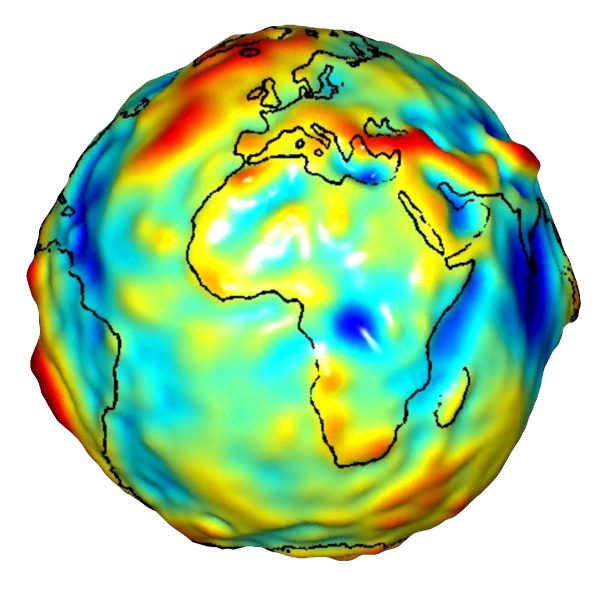
\includegraphics[width=.4\mycolumnwidth]{Fundamentos_cartograficos/Geoide.png}
\caption{\small Representaci�n gr�fica del geoide (Fuente: Misi�n GRACE (NASA)).}
\label{Fig:Geoide} 
\end{figure}

L�gicamente, el elipsoide, por su naturaleza m�s simple, no puede recoger toda la variabilidad del geoide, por lo que estas dos superficies presentan diferencias, cuyo m�ximo es generalmente del orden de $\pm100$ metros. Estas diferencias se conocen como \emph{alturas geoidales}.\index{Alturas geoidales}

Al igual que en el caso de los elipsoides, existen diversos geoides de referencia, y estos no son constantes en el tiempo sino que evolucionan para adaptarse a las modificaciones que tienen lugar sobre la superficie terrestre.

La figura \ref{Fig:Tres_superficies} muestra una comparaci�n esquem�tica entre las tres superficies: superficie real de la Tierra, geoide y elipsoide.

\begin{figure}
\centering
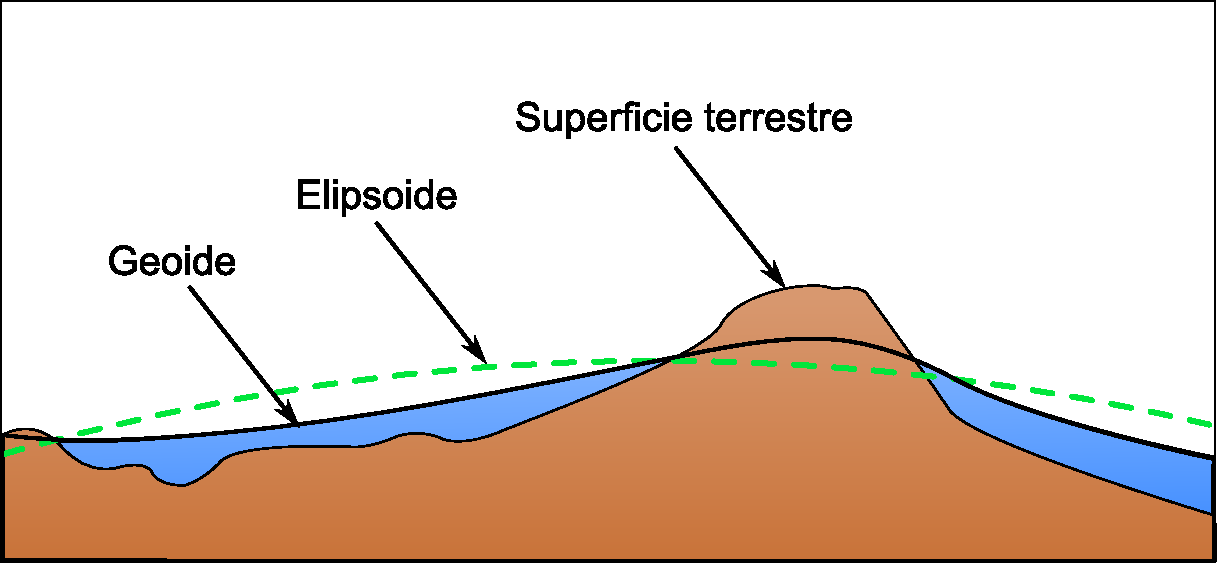
\includegraphics[width=.6\mycolumnwidth]{Fundamentos_cartograficos/Tres_superficies.pdf}
\caption{\small Tres superficies fundamentales: superficie real de la Tierra, geoide y elipsoide (Adaptado de Wikipedia).}
\label{Fig:Tres_superficies} 
\end{figure}

\subsection{El datum geod�sico}

\index{Datum geod�sico}

Cuando se trabaja con un elipsoide general, este, como se ha dicho, se sit�a de tal modo que tanto la posici�n de su centro de gravedad como su plano ecuatorial coincidan con los terrestres. Por el contrario, cuando el elipsoide es local, estas propiedades no han de cumplirse necesariamente, y el elipsoide a solas resulta insuficiente ya que carecemos de informaci�n sobre su posicionamiento con respecto a la superficie terrestre.

Surge as� el concepto de \emph{datum}, que es el conjunto formado por una superficie de referencia (el elipsoide) y un punto en el que <<enlazar>> este al geoide. Este punto se denomina \emph{punto astron�mico fundamental}\index{Punto astron�mico fundamental} (para su c�lculo se emplean m�todos astron�micos), o simplemente \emph{punto fundamental}, y en �l el elipsoide es tangente al geoide. La altura geoidal en este punto es, como cabe esperar, igual a cero. La vertical al geoide y al elipsoide son id�nticas en el punto fundamental.

Para un mismo elipsoide pueden utilizarse distintos puntos fundamentales, que dar�n lugar a distintos datum y a distintas coordenadas para un mismo punto.

%*****************

\section{Sistemas de coordenadas}

\index{Coordenadas!sistemas de}
Disponiendo de un modelo preciso para definir la forma de la Tierra, podemos establecer ya un sistema de codificar cada una de las posiciones sobre su superficie y asignar a estas las correspondientes coordenadas. Puesto que la superficie de referencia que consideramos es un elipsoide, lo m�s l�gico es recurrir a los elementos de la geometr�a esf�rica y utilizar estos para definir el sistema de referencia. De ellos derivan los conceptos de latitud y longitud, empleados para establecer las \emph{coordenadas geogr�ficas}\index{Coordenadas!geogr�ficas} de un punto.

No obstante, la geometr�a plana resulta mucho m�s intuitiva y pr�ctica que la geometr�a esf�rica para realizar ciertas tareas, y a ra�z de esto surgen las \emph{proyecciones cartogr�ficas}\index{Proyecci�n}, que tratan de situar los elementos de la superficie del elipsoide sobre una superficie plana, y que son los que se emplean para la creaci�n de cartograf�a. Al aplicar una proyecci�n cartogr�fica, las coordenadas resultantes son ya coordenadas cartesianas.

Ambas formas de expresar la posici�n de un punto son utilizadas en la actualidad, y las veremos con detalle en esta secci�n.

\subsection{Coordenadas geogr�ficas}

El sistema de coordenadas geogr�ficas es un sistema de coordenadas esf�ricas mediante el cual un punto se localiza con dos valores angulares: 

\begin{itemize}
	\item la \emph{latitud}\index{Latitud} $\phi$ es el �ngulo entre la l�nea que une el centro de la esfera con un punto de su superficie y el plano ecuatorial. Las lineas formadas por puntos de la misma latitud se denominan \emph{paralelos}\index{Paralelo} y forman c�rculos conc�ntricos paralelos al ecuador. Por definici�n la latitud es de 0\degree en el ecuador, que divide el globo en los hemisferios norte y sur. La latitud puede expresarse especificando si el punto se sit�a al norte o al sur, por ejemplo 24\degree, 21' 11'' N, o bien utilizando un signo, en cuyo caso los puntos al Sur del ecuador tienen signo negativo.
	\item la \emph{longitud}\index{Longitud (geogr�fica)} $\lambda$ La longitud es el angulo formado entre dos de los planos que contienen a la linea de los Polos. El primero es un plano arbitrario que se toma como referencia y el segundo es el que, ademas de contener a la linea de los polos, contiene al punto en cuesti�n. Las l�neas formadas por puntos de igual longitud se denominan \emph{meridianos}\index{Meridiano} y convergen en los polos.
	
	Como meridiano de referencia internacional se toma aquel que pasa por el observatorio de Greenwich\index{Greenwich (meridiano)}, en el Reino Unido. Este divide a su vez el globo en dos hemisferios: el Este y el Oeste. La longitud puede expresarse especificando si el punto se sit�a al Este o al Oeste, por ejemplo 32\degree, 12' 43'' E, o bien utilizando un signo, en cuyo caso los puntos al Oeste del meridiano de referencia tienen signo negativo.
\end{itemize}

En la figura \ref{Fig:Coordenadas_geograficas} puede verse un esquema de los conceptos anteriores.

\begin{figure}
\centering
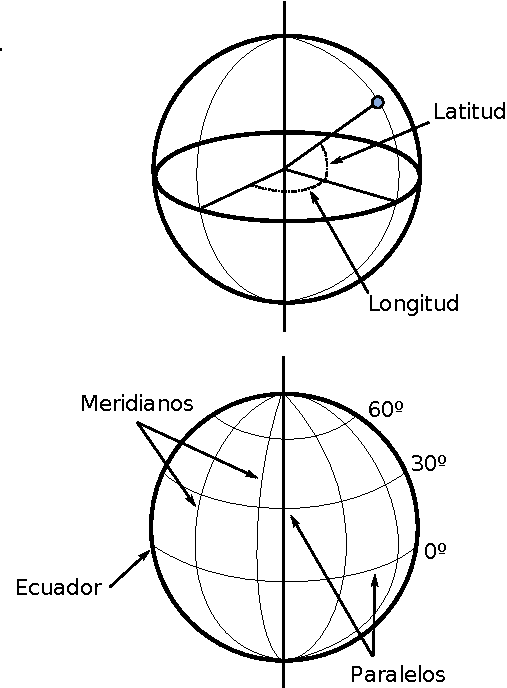
\includegraphics[width=.5\mycolumnwidth]{Fundamentos_cartograficos/Coordenadas_geograficas.pdf}
\caption{\small Esquema de los elementos del sistema de coordenadas geogr�ficas.}
\label{Fig:Coordenadas_geograficas} 
\end{figure}

La tabla \ref{Tabla:Coordenadas_ciudades} recoge las coordenadas geogr�ficas de algunas ciudades importantes, a modo de ejemplo.

\begin{table}
\begin{center}
\begin{tabular}{ccc}\toprule
\textsf{Ciudad} & \textsf{Latitud} & \textsf{Longitud}  \\ \midrule
Badajoz & 38.53 N & 6.58 O \\
Barcelona & 41.23 N & 2.11 E \\
Cadiz & 36.32 N & 6.18 O \\
Girona & 41.59 N & 2.49 E \\
Granada & 37.11 N & 3.35 O\\
Madrid & 40.24 N & 3.41 O\\
Segovia & 40.57 N & 4.07 O \\
Valencia & 39.28 N & 0.22 O\\
Zaragoza & 41.39 N & 0.52 O \\ \bottomrule
\end{tabular}
\end{center}
\caption{\small Coordenadas geogr�ficas de algunas ciudades}
\label{Tabla:Coordenadas_ciudades}
\end{table}

Las coordenadas geogr�ficas resultan de gran utilidad, especialmente cuando se trabaja con grandes regiones. No obstante, no se trata de un sistema cartesiano, y tareas como la medici�n de �reas o distancias es mucho m�s complicada. Si bien la distancia entre dos paralelos es pr�cticamente constante (es decir, un grado de latitud equivale m�s o menos a una misma distancia en todos los puntos), la distancia entre dos meridianos no lo es, y var�a entre unos 11,3 kil�metros en el Ecuador hasta los cero kil�metros en los polos, donde los meridianos convergen. \index{Distancia!entre meridianos}

\subsection{Proyecciones cartogr�ficas}

\index{Proyecci�n}

A pesar de su innegable utilidad y la potencia que nos brindan para la localizaci�n de cualquier punto sobre la superficie terrestre, un sistema de coordenadas esf�ricas tiene inconvenientes que no pueden obviarse. Por una parte, estamos m�s acostumbrados a la utilizaci�n de sistemas cartesianos en los cuales la posici�n de un punto se define mediante un par de medidas de distancia $x$ e $y$. Esta forma es mucho m�s sencilla e intuitiva, y permite una mayor facilidad de operaciones.

Por otro lado, si necesitamos crear una representaci�n visual de la informaci�n cartogr�fica, lo habitual es hacerlo en una superficie plana, ya sea a la manera cl�sica en un pliego de papel o, usando las tecnolog�as actuales, en un dispositivo tal como una pantalla.

Por todo ello, se deduce que existe una necesidad de poder trasladar la informaci�n geogr�fica (incluyendo, por supuesto, la referente a su localizaci�n) a un plano, con objeto de poder crear cartograf�a y simplificar gran n�mero de operaciones posteriores. El proceso de asignar una coordenada plana a cada punto de la superficie de la Tierra (que no es plana) se conoce como \emph{proyecci�n cartogr�fica}.

M�s exactamente, una \textit{proyecci�n cartogr�fica} es la correspondencia matem�tica biun�voca entre los puntos de una esfera o elipsoide y sus transformados en un plano \cite{Martin1983IGN}. Es decir, una aplicaci�n $f$ que a cada par de coordenadas geogr�ficas $(\phi, \lambda)$ le hace corresponder un par de coordenadas cartesianas $(x, y)$, seg�n

\begin{equation}\label{Eq:Proyecciones}
x = f(\phi, \lambda) \; ; \; y = f(\phi, \lambda)
\end{equation}

De igual modo, las coordenadas geogr�ficas puede obtenerse a partir de las cartesianas seg�n

\begin{equation}\label{Eq:Proyecciones2}
\phi = g(x,y) \; ; \; \lambda = g(x,y)
\end{equation}

Se puede pensar que podemos obtener una representaci�n plana de la superficie de una esfera o un elipsoide si tomamos esta y la extendemos hasta dejarla plana. Esto, sin embargo, no resulta posible, ya que dicha superficie no puede \emph{desarrollarse} y quedar plana. Por ello, hay que buscar una forma distinta de relacionar los puntos en la superficie tridimensional con nuevos puntos en un plano. \index{Superficie!desarrollable}

La figura \ref{Fig:Proyeccion} muestra un esquema del concepto de proyecci�n, esbozando la idea de c�mo puede establecerse la correspondencia entre puntos de la esfera y del plano.

\begin{figure}
\centering
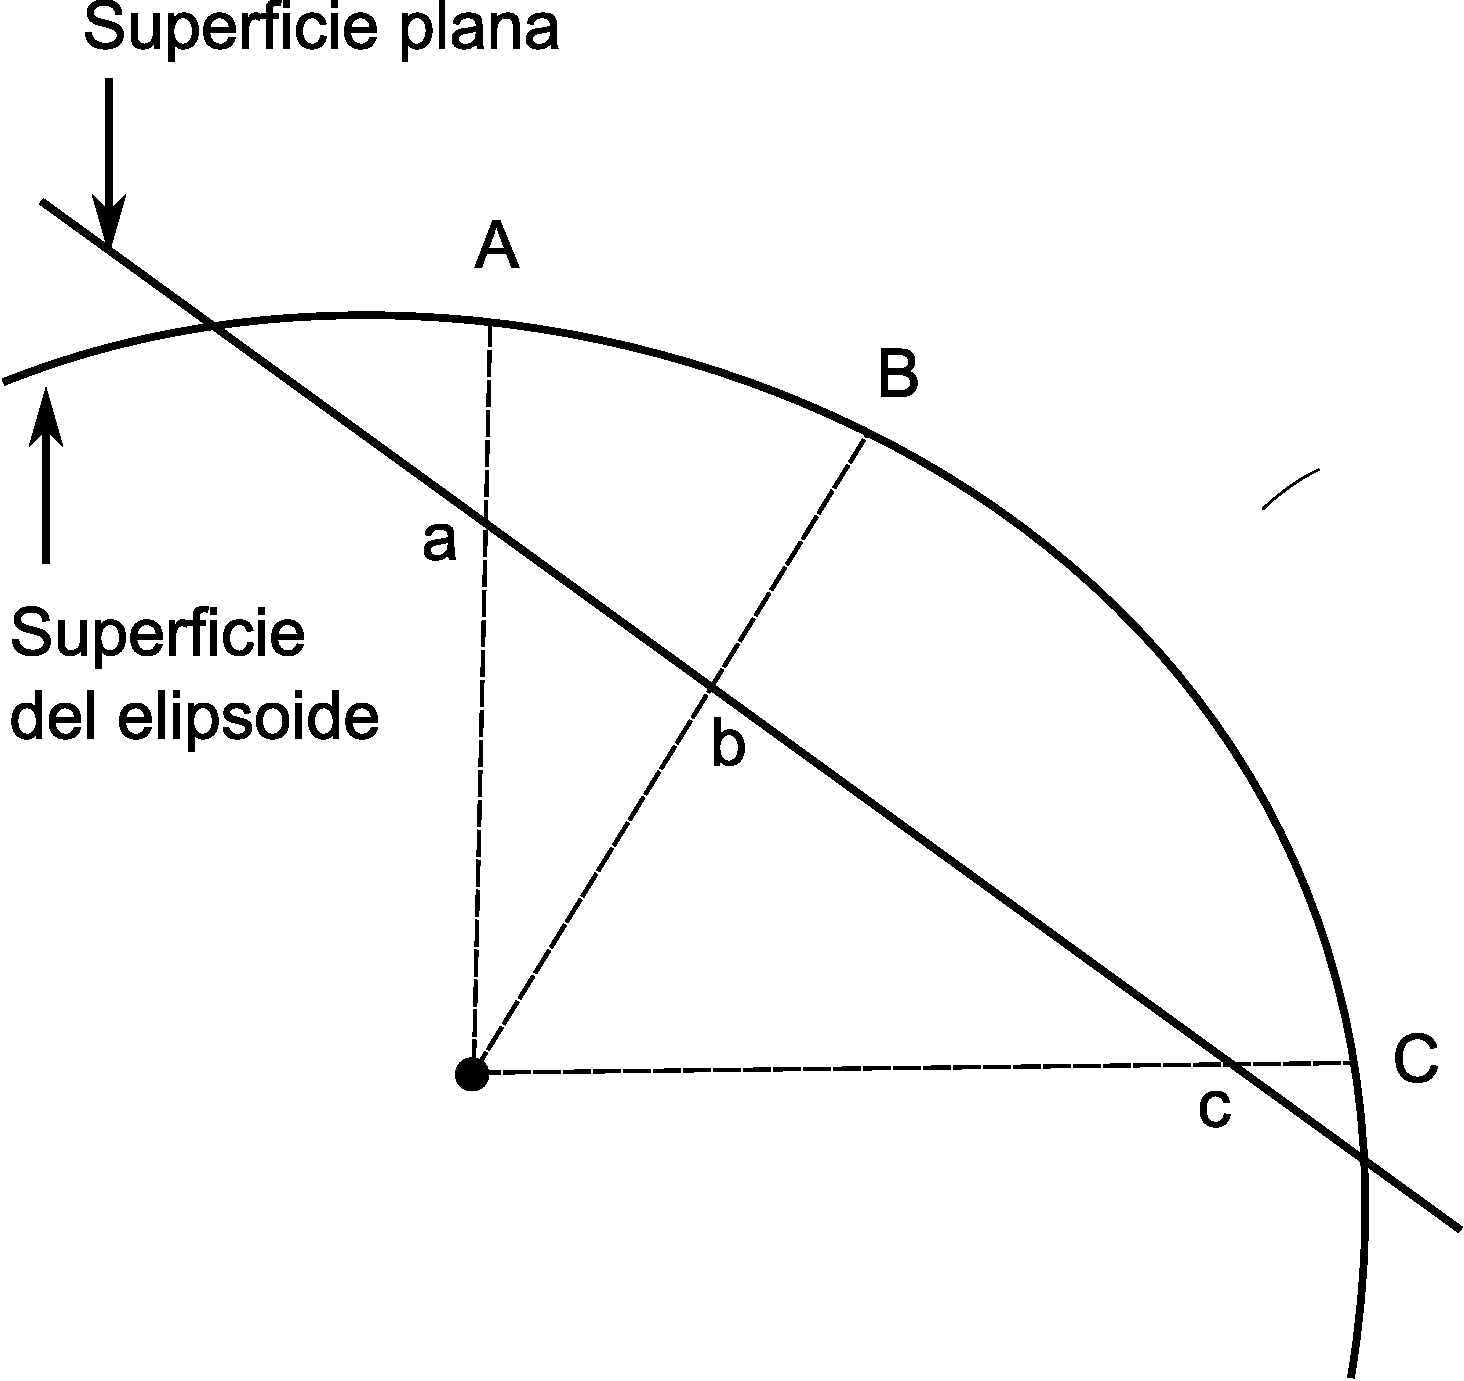
\includegraphics[width=.5\mycolumnwidth]{Fundamentos_cartograficos/Proyeccion.pdf}
\caption{\small Esquema del concepto de proyecci�n. A los puntos $A, B$ y $C$ sobre la superficie del elipsoide les asocian equivalentes $a, b$ y $c$ sobre un plano.}
\label{Fig:Proyeccion} 
\end{figure}

En ella vemos c�mo el concepto de proyecci�n se asemeja a la generaci�n de sombras, ya que a partir de un foco se trazan las trayectorias de una serie de rayos que unen dicho foco con los puntos a proyectar, y despu�s se determina el punto de contacto de esos rayos con la superficie plana. Aunque no todas las proyecciones siguen necesariamente este esquema, una parte de ellas s� que se fundamentan en un razonamiento similar a este, y el esquema mostrado sirve bien para entender el concepto y el paso de coordenadas de una superficie tridimensional a una bidimensional.

Veremos en los siguientes puntos las diferentes modificaciones que pueden introducirse sobre la forma anterior de proyectar, y que dan lugar a tipos distintos de proyecciones.

Puede apreciarse igualmente en la figura que se producen distorsiones al realizar la proyecci�n. Es decir, que ciertas propiedades no se reproducen con fidelidad al pasar puntos desde la superficie curva al plano. Por ejemplo, la distancia entre los puntos $A$ y $B$ no es igual a la existente entre los puntos $a$ y $b$. Con independencia de las caracter�sticas propias de la proyecci�n, siempre existen distorsiones. Esto es as� debido a que la esfera, como se ha dicho, no es desarrollable, mientras que el plano s� lo es, y por ello en el paso de coordenadas de uno a otra han de aparecen inevitablemente alteraciones.

%Para resumir todo lo visto hasta el momento, la figura \ref{Fig:Elementos_para_crear_proyecciones} muestra un resumen esquem�tico de c�mo a partir de la superficie terrestre, y con los elementos que hemos desarrollado en este cap�tulo, se obtienen las representaciones planas.
%
%
%\begin{figure}
%\centering
%\includegraphics[width=.75\textwidth]{Fundamentos_cartograficos/Elementos_para_crear_proyecciones.pdf}
%\caption{\small Resumen esquem�tico del proceso que va desde la concepci�n de la superficie terrestre hasta la creaci�n de una representaci�n plana mediante la aplicaci�n de una proyecci�n cartogr�fica.}
%\label{Fig:Elementos_para_crear_proyecciones} 
%\end{figure}

\subsubsection{Tipos de proyecciones}\label{TiposProyecciones}

Las proyecciones se clasifican seg�n la superficie sobre la que se proyectan los puntos. En el esquema de la figura \ref{Fig:Proyeccion}, el plano de proyecci�n es ya de por s� bidimensional. No obstante, puede realizarse la proyecci�n sobre una superficie tridimensional, siempre que esta, a diferencia de la esfera, s� sea desarrollable. Es decir, que pueda <<desenrollarse>> y convertirse en un plano sin necesidad de doblarse o cortarse. Estas otras superficies pueden emplearse tambi�n para definir una proyecci�n, de la misma forma que se hace con un plano.

Las superficies m�s habituales son el cono y el cilindro (junto con, por supuesto, el plano), las cuales, situadas en una posici�n dada en relaci�n al objeto a proyectar (esto es, la Tierra), definen un tipo dado de proyecci�n. Distinguimos as� los siguiente tipos de proyecciones:

\index{Punto de fuga}

\begin{itemize}
\item C�nicas.\index{Proyecci�n geogr�fica!C�nica} La superficie desarrollable es un cono (Figura \ref{Fig:Proyeccion_conica}), que se sit�a generalmente tangente o secante en dos paralelos a la superficie del elipsoide. En este �ltimo caso, la distorsi�n se minimiza en las �reas entre dichos paralelos, haci�ndola �til para representar franjas que no abarquen una gran distancia en latitud, pero poco adecuada para representaci�n de grandes �reas. Algunas de las proyecciones m�s conocidas de este grupo son la proyecci�n c�nica equi�rea de Albers\index{Proyecci�n geogr�fica!equi�rea de Albers} y la proyecci�n conforme c�nica de Lambert.

\begin{figure}
\centering
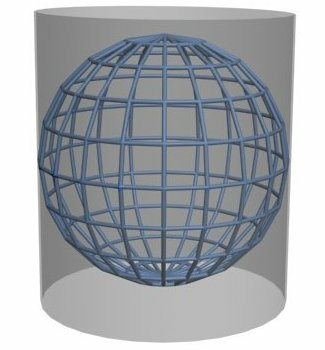
\includegraphics[width=.35\mycolumnwidth]{Fundamentos_cartograficos/Proyeccion_cilindrica.png}
\caption{\small Esquema de una proyecci�n cil�ndrica (tomado de Wikipedia)}
\label{Fig:Proyeccion_cilindrica} 
\end{figure}


\item Cil�ndricas. La superficie desarrollable es un cilindro (Figura \ref{Fig:Proyeccion_cilindrica}). Al proyectar, los meridianos se convierten en lineas paralelas, as� como los paralelos, aunque la distancia entre estos �ltimos no es constante.

En su concepci�n m�s simple, el cilindro se sit�a de forma tangente al ecuador (proyecci�n normal o simple), aunque puede situarse secante y hacerlo a los meridianos (proyecci�n transversa) o a otros puntos (proyecci�n oblicua).

La proyecci�n de Mercator, la transversa de Mercator, la cil�ndrica de Miller\index{Proyecci�n geogr�fica!cil�ndrica de Miller} o la cil�ndrica equi�rea de Lambert\index{Proyecci�n geogr�fica!cil�ndrica de Miller} son ejemplos relativamente comunes de este tipo de proyecciones.

\begin{figure}
\centering
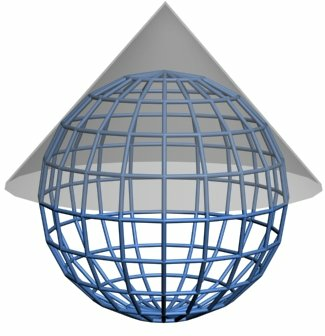
\includegraphics[width=.35\mycolumnwidth]{Fundamentos_cartograficos/Proyeccion_conica.png}
\caption{\small Esquema de una proyecci�n c�nica (tomado de Wikipedia)}
\label{Fig:Proyeccion_conica} 
\end{figure}


\item Planas o azimutales. \index{Proyecci�n geogr�fica!plana}La superficie desarrollable es directamente un plano. Seg�n el esquema de la figura \ref{Fig:Proyeccion}, tenemos distintos tipos en funci�n de la posici�n del punto de fuga.

\begin{itemize}
\item Gn�mica o central. El punto de fuga se sit�a en el centro del elipsoide. \index{Proyecci�n geogr�fica!gn�mica}
\item Estereogr�fica. El plano es tangente y el punto de fuga se sit�a en las ant�podas del punto de tangencia. La proyecci�n polar estereogr�fica es empleada habitualmente para cartografiar las regiones polares. \index{Proyecci�n geogr�fica!estereogr�fica}
\item Ortogr�fica. El punto de fuga se sit�a en el infinito. \index{Proyecci�n geogr�fica!ortogr�fica}
\end{itemize}

Existen proyecciones azimutales que no son de tipo perspectivo, es decir, que no se basan en el esquema de la figura \ref{Fig:Proyeccion}. La proyecci�n de Airy, por ejemplo, es una de ellas.

\item Algunas proyecciones no se ajustan exactamente al esquema planteado, y no utilizan una superficie desarrollable como tal sino modificaciones a esta idea. Por ejemplo, las proyecciones \emph{polic�nicas}\index{Proyecci�n geogr�fica!polic�nica} utilizan la misma filosof�a que las c�nicas, empleando conos, pero en lugar de ser este �nico, se usan varios conos, cada uno de los cuales se aplica a una franja concreta de la zona proyectada. La uni�n de todas esas franjas, cada una de ellas proyectada de forma distinta (aunque siempre con una proyecci�n c�nica), forma el resultado de la proyecci�n.

Del mismo modo, encontramos proyecciones como la proyecci�n \emph{sinusoidal}\index{Proyecci�n geogr�fica!sinusoidal}, una proyecci�n de tipo pseudocil�ndrico, o la proyecci�n de Werner, cuya superficie desarrollable tiene forma de coraz�n. Estas proyecciones son, no obstante, de uso menos habitual, y surgen en algunos casos como respuesta a una necesidad cartogr�fica concreta.
\end{itemize}

Otra forma distinta de clasificar las proyecciones es seg�n las propiedades m�tricas que conserven. Toda proyecci�n implica alguna distorsi�n (denominada \emph{anamorfosis})\index{Anamorfosis}, y seg�n c�mo sea esta y a qu� propiedad m�trica afecte o no, podemos definir los siguientes tipos de proyecciones:

\begin{itemize}
\item Equi�rea. En este tipo de proyecciones se mantiene una escala constante. Es decir, la relaci�n entre un �rea terrestre y el �rea proyectada es la misma independientemente de la localizaci�n, con lo que la representaci�n proyectada puede emplearse para comparar superficies.
\item Conformes. Estas proyecciones mantienen la forma de los objetos, ya que no provocan distorsi�n de los �ngulos. Los meridianos y los paralelos se cortan en la proyecci�n en �ngulo recto, igual que sucede en la realidad. Su principal desventaja es que introducen una gran distorsi�n en el tama�o, y objetos que aparecen proyectados con un tama�o mucho mayor que otros pueden ser en la realidad mucho menores que estos.
\item Equidistantes. En estas proyecciones se mantienen las distancias.
\end{itemize}

En los ejemplos de proyecciones que se han citado para los distintos tipos de proyecciones (c�nicas, cil�ndricas, etc.) puede verse c�mo resulta com�n especificar el tipo en funci�n de la propiedad m�trica preservada, para as� caracterizar completamente la proyecci�n.

La elecci�n de una u otra proyecci�n es funci�n de las necesidades particulares. Como ya se ha dicho, la proyecci�n polar estereogr�fica es empleada cuando se trabaja las regiones polares, ya que en este caso es la m�s adecuada. Proyecciones como la de Mercator, empleadas habitualmente, no resultan tan adecuadas en esas zonas. Asimismo, hay proyecciones que no pueden recoger todo el globo, sino solo una parte de este, por lo que no son de aplicaci�n para grandes escalas. La existencia de un gran n�mero de distintas proyecciones es precisamente fruto de las diferentes necesidades que aparecen a la hora de trabajar con cartograf�a.

\subsection{El sistema UTM}

\index{Proyecci�n geogr�fica!UTM}

De entre los cientos proyecciones de existen actualmente, algunas tienen un uso m�s extendido, bien sea por su adopci�n de forma estandarizada o sus propias caracter�sticas. Estas proyecciones, que se emplean con m�s frecuencia para la creaci�n de cartograf�a, son tambi�n las que m�s habitualmente vamos a encontrar en los datos que empleemos con un SIG, y es por tanto de inter�s conocerlas un poco m�s en detalle.

En la actualidad, una de las proyecciones m�s extendidas en todos los �mbitos es la proyecci�n universal transversa de Mercator, la cual da lugar al sistema de coordenadas UTM. Este sistema, desarrollado por el ej�rcito de los Estados Unidos, no es simplemente una proyecci�n, sino que se trata de un sistema completo para cartografiar la practica totalidad de la Tierra. Para ello, esta se divide en una serie de zonas rectangulares mediante una cuadricula y se aplica una proyecci�n y unos par�metros geod�sicos concretos a cada una de dichas zonas. Aunque en la actualidad se emplea un �nico elipsoide (WGS--84)\index{WGS--84}, originalmente este no era �nico para todas las zonas.

Con el sistema UTM, las coordenadas de un punto no se expresan como coordenadas terrestres absolutas, sino mediante la zona correspondiente y las coordenadas relativas a la zona UTM en la que nos encontremos.

La cuadricula UTM tiene un total de 60 husos\index{Huso} numerados entre 1 y 60, cada uno de los cuales abarca una amplitud de 6\degree de longitud. El huso 1 se sit�a entre los 180\degree y 174\degree O, y la numeraci�n avanza hacia el Este. 

En latitud, cada huso se divide en 20 zonas, que van desde los 80\degree S hasta los 84\degree N. Estas se codifican con letras desde la C a la X, no utiliz�ndose las letras I y O por su similitud con los d�gitos 1 y 0. Cada zona abarca 8 grados de longitud, excepto la X que se prolonga unos 4 grados adicionales. 

La figura \ref{Fig:Zonas_UTM} muestra un esquema de la cuadr�cula UTM.

\begin{figure}
\centering
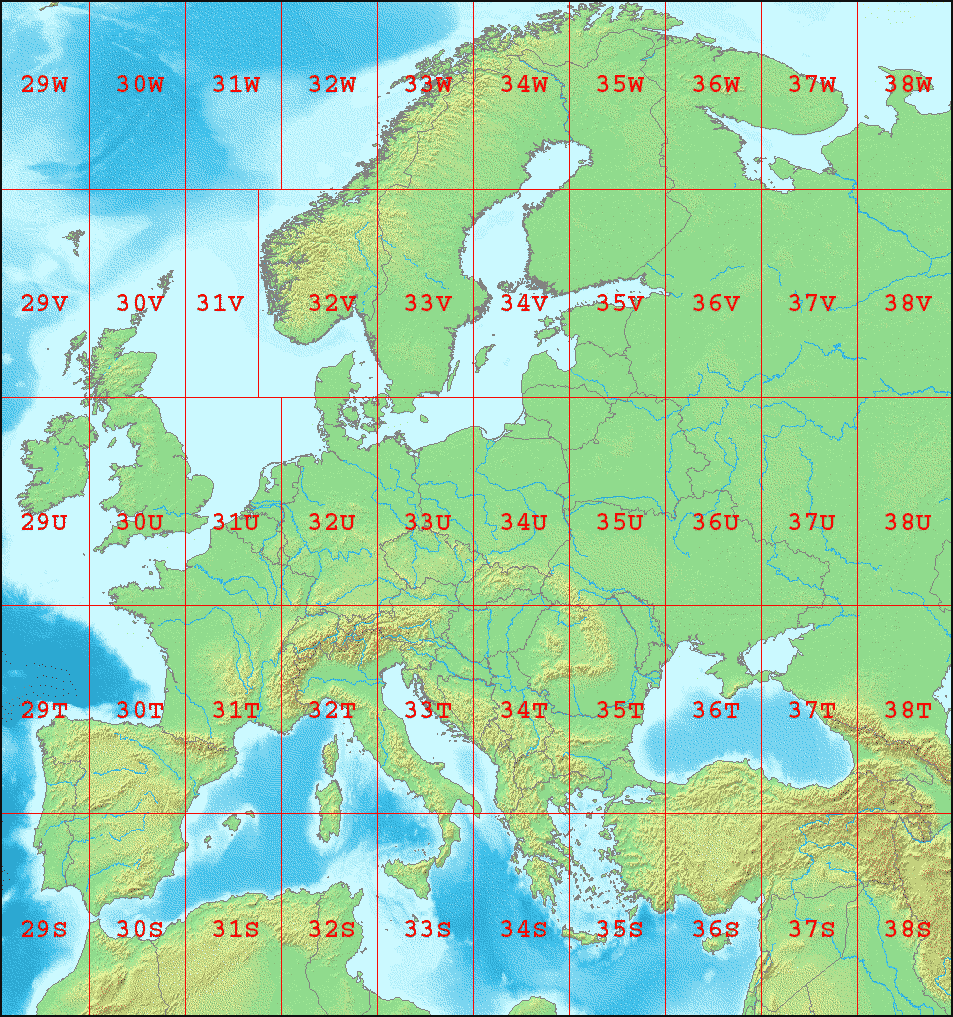
\includegraphics[width=.6\mycolumnwidth]{Fundamentos_cartograficos/Zonas_UTM.png}
\caption{\small Representaci�n parcial de la cuadr�cula UTM en Europa (tomado de Wikipedia)}
\label{Fig:Zonas_UTM} 
\end{figure}

Una zona UTM se localiza, por tanto, con un n�mero y una letra, y es en funci�n de la zona como posteriormente se dan las coordenadas que localizan un punto. Estas coordenadas se expresan en metros y expresan la distancia entre el punto y el origen de la zona UTM en concreto. El origen de la zona se sit�a en el punto de corte entre el meridiano central de la zona y el ecuador. Por ejemplo, para las zonas UTM en el huso 31, el cual va desde los 0\degree hasta los 6\degree, el origen se sit�a en el punto de corte entre el ecuador y el meridiano de 3\degree (Figura \ref{Fig:Origen_UTM}).

\begin{figure}
\centering
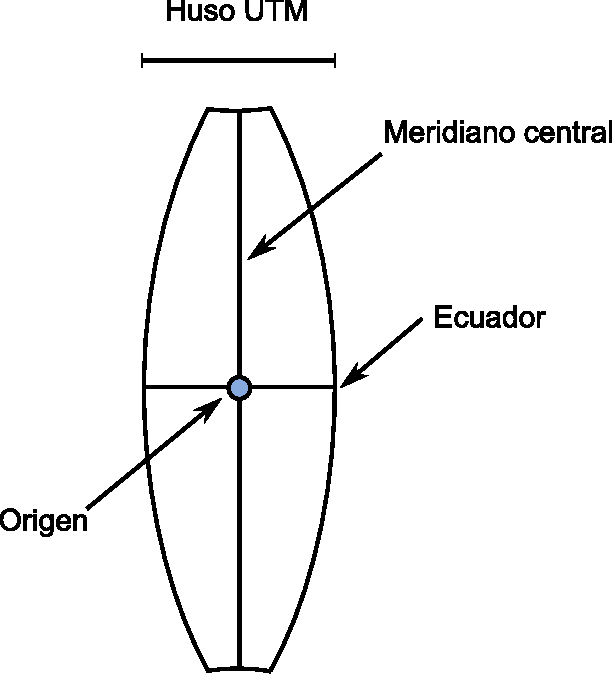
\includegraphics[width=.35\mycolumnwidth]{Fundamentos_cartograficos/Origen_UTM.pdf}
\caption{\small Determinaci�n del origen de una zona UTM}
\label{Fig:Origen_UTM} 
\end{figure}

Para evitar la aparici�n de n�meros negativos, se considera que el origen no tiene una coordenada X de 0 metros, sino de 500000. Con ello se evita que las zonas al Este del meridiano central tengan coordenadas negativas, ya que ninguna zona tiene un ancho mayor de 1000000 metros (el ancho es m�ximo en las zonas cerca del ecuador, siendo de alrededor de 668 kil�metros).

De igual modo, cuando se trabaja en el hemisferio sur (donde las coordenadas Y ser�an siempre negativas), se considera que el origen tiene una coordenada Y de 10000000 metros, lo cual hace que todas las coordenadas referidas a �l sean positivas.

Para las zonas polares no resulta adecuado emplear el sistema UTM, ya que las distorsiones que produce son demasiado grandes. En su lugar, se utiliza el sistema UPS (Universal Polar Stereographic). \index{Proyecci�n geogr�fica!UPS}

\subsection{Transformaci�n y conversi�n de coordenadas}

Una situaci�n muy habitual en el trabajo con un SIG es disponer de cartograf�a en varios sistemas de coordenadas en un mismo sistema pero con par�metros diferentes (por ejemplo, diferente datum). Para poder emplear toda esa cartograf�a de forma conjunta, resulta necesario trabajar en un sistema �nico y bien definido, lo cual hace necesario convertir al menos una parte de ella. 

Este cambio de coordenadas puede ser obligatorio a cualquier escala de trabajo, ya que las diferencias en el sistema escogido pueden aparecer por circunstancias muy diversas, incluso si todos los datos tienen un origen com�n. As�, al reunir informaci�n de varios pa�ses para crear en un SIG un mapa de todo un continente, es probable que los datos de cada pa�s est�n referidos a un sistema distinto, pero incluso trabajando en un �rea m�s reducida podemos encontrar una situaci�n similar. En Espa�a, por ejemplo, podemos encontrar cartograf�a de algunas Comunidades Aut�nomas en dos husos UTM distintos, ya que la frontera entre estos cruza y divide dichas Comunidades.

Distinguimos dos tipos de operaciones a realizar con coordenadas:

\begin{itemize}
	\item Conversi�n de coordenadas. Los sistemas de origen y destino comparten el mismo datum. Es una transformaci�n exacta y se basa en la aplicaci�n de formulas establecidas que relacionan ambos sistemas.
	\item Transformaci�n de coordenadas. El datum es distinto en los sistemas de origen y destino.
\end{itemize}

\index{Transformaci�n!de coordenadas}\index{Conversi�n!de coordenadas}\index{Coordenadas!transformaci�n}\index{Coordenadas!conversi�n}

Las proyecciones cartogr�ficas, vistas en un punto anterior, son una forma particular de conversi�n de coordenadas.

Un SIG ha de estar preparado para trabajar con cartograf�a en cualquiera de los sistemas de referencia m�s habituales y, m�s a�n, para facilitar al usuario la utilizaci�n de todo tipo de informaci�n geogr�fica con independencia del sistema de coordenadas que se emplee. Para ello, los SIG incorporan los procesos necesarios para efectuar cambios de coordenadas, de forma que para unos datos de partida se genera un nuevo conjunto de datos con la misma informaci�n pero expresada en un sistema de coordenadas distinto.

Otra forma en la que los SIG pueden implementar estas operaciones es mediante capacidades de transformaci�n y conversi�n <<al vuelo>>\index{Transformaci�n!al vuelo}, es decir, en tiempo real. De este modo, pueden introducirse en un SIG datos en sistemas de coordenadas variados, y el SIG se encarga de cambiar estos a un sistema de referencia base fijado de antemano. Este proceso tiene lugar de forma transparente para el usuario, que tiene la sensaci�n de que todos los datos estaban originalmente en el sistema de trabajo escogido.

Esto exige, l�gicamente, que todo dato geogr�fico se acompa�e de informaci�n acerca del sistema de coordenadas que se ha utilizado para crearlo, algo que no siempre sucede. Veremos m�s acerca de la importancia de este tipo de informaci�n adicional en el cap�tulo \ref{Metadatos}.

\subsection{Codificaci�n de sistemas de referencia}

Debido al elevado n�mero de distintos sistemas de referencia existentes, resulta f�cil perderse en ellos a la hora de tener que trabajar con cartograf�a en distintos sistemas. Si bien es cierto que existe un esfuerzo integrador para tratar de homogeneizar el uso de sistemas de referencia, tambi�n existen esfuerzos para intentar facilitar la gesti�n de estos y que no resulte tan complejo combinar cartograf�a producida utilizando sistemas de coordenadas diferentes.

Uno de los intentos m�s exitosos en este sentido es el desarrollado por el consorcio petrol�fero European Petroleum Survey Group (EPSG)\index{European Petroleum Survey Group (EPSG)}, el cual, consciente de la necesidad de disponer de informaci�n acerca de los distintos sistemas de coordenadas y de que esta informaci�n fuera de f�cil acceso y manejo, ha elaborado un esquema de codificaci�n espec�fico. 

\index{EPSG, c�digos}\index{European Petroleum Survey Group}

Este esquema asocia a cada sistema de coordenadas un c�digo (conocido como \emph{c�digo EPSG}) que la identifica. Paralelamente, se han documentado en un formato com�n las caracter�sticas principales de todos estos sistemas, as� como las formulaciones que permiten transformar coordenadas entre ellos.

Esta informaci�n constituye el \emph{EPSG geodetic parameter dataset}, un repositorio de los par�metros necesarios para \cite{webEPSG}

\begin{itemize}
	\item identificar coordenadas de tal modo que estas describan la posici�n de un punto de forma inequ�voca y no ambigua.
	\item definir transformaciones y conversiones que permitan pasar de un sistema de referencia a otro.
\end{itemize}

Informaci�n detallada sobre los c�digos EPSG puede encontrarse en \cite{webEPSG}.

\section{Escala}\label{Escala}
\index{Escala}

El concepto de escala es fundamental a la hora de trabajar con cartograf�a, y es uno de los valores b�sicos que definen toda representaci�n cartogr�fica. Esta representaci�n ha de tener un tama�o final manejable, con objeto de que pueda resultar de utilidad y permitir un uso pr�ctico, pero el objeto que se cartograf�a (un pa�s, un continente o bien la Tierra al completo) es un objeto de gran tama�o. Esto hace necesario que, para crear un mapa, se deba reducir o bien el objeto original o bien el objeto ya proyectado, dando lugar a una versi�n <<reducida>> que ya cumple con los requisitos de tama�o adecuado.

Es decir, imaginemos que aplicamos una proyecci�n c�nica sobre el elipsoide, empleando para ello un cono que cubra dicho elipsoide, el cual tendr� que ser, l�gicamente de gran tama�o (�hay que cubrir toda la Tierra!). Al desarrollarlo, el plano que obtenemos tiene miles de kil�metros de lado. Debemos fabricar una versi�n <<a escala>> de este, que ser� la que ya podamos utilizar.

En este contexto, la escala no es sino la relaci�n de tama�o existente entre ese gran mapa que se obtiene al desarrollar nuestro cono de proyecci�n y el que finalmente manejamos, de tama�o m�s reducido. Conociendo esta relaci�n podemos ya conocer las verdaderas magnitudes de los elementos que vemos en el mapa, ya que podemos convertir las medidas hechas sobre el mapa en medidas reales. Es importante recordar que esas medidas no son tan <<reales>>, puesto que la propia proyecci�n las ha distorsionado ---lo cual no debe olvidarse---, pero s� que son medidas en la escala original del objeto cartografiado.

La escala se expresa habitualmente como un denominador que relaciona una distancia medida en un mapa y la distancia que esta medida representa en la realidad. Por ejemplo, una escala 1:50000 quiere decir que 1 cent�metro en un mapa equivale a 50000 cent�metros en la realidad, es decir a 500 metros. Conociendo este valor de la escala podemos aplicar sencillas reglas de tres para calcular la distancia entre dos puntos o la longitud de un elemento dado, sin m�s que medirlo sobre el mapa y despu�s convertir el resultado obtenido en una medida real.

Una vez m�s es preciso insistir que lo anterior es posible siempre bajo las limitaciones que la propia proyecci�n empleada para crear el mapa tenga al respecto, y que depender�n del tipo de proyecci�n que sea en funci�n de las propiedades m�tricas que conserva.

De hecho, e independientemente del tipo de proyecci�n, la escala es completamente cierta �nicamente en determinadas partes del mapa. Cuando decimos que un mapa tiene una escala 1:50000, este valor, denominado \emph{Escala Num�rica}, se cumple con exactitud tan solo en algunos puntos o l�neas. En otros puntos la escala var�a. La relaci�n entre la escala en esos puntos y la Escala Num�rica se conoce como \emph{Factor de Escala}. \index{Escala!factor de}

A pesar de que la escala es imprescindible para darle un uso pr�ctico a todo mapa, y cualquier usuario de este debe conocer y aplicar el concepto de escala de forma precisa, los SIG pueden resultar enga�osos al respecto. Aunque la escala como idea sigue siendo igual de fundamental cuando trabajamos con informaci�n geogr�fica en un SIG, las propias caracter�sticas de este y la forma en la que dicha informaci�n se incorpora en el SIG pueden hacer que no se perciba la escala como un concepto tan relevante a la hora de desarrollar actividad con �l.

Esto es debido principalmente a que la escala tiene una relaci�n directa con la visualizaci�n, ya que se establece entre la realidad y una representaci�n visual particular, esto es, el mapa. Como ya se ha mencionado en el cap�tulo \ref{Introduccion_fundamentos}, los datos en un SIG tienen car�cter num�rico y no visual, y la representaci�n de estos se encarga de realizarla el subsistema correspondiente a partir de dichos datos num�ricos. Es decir, que en cierta medida en un SIG no es estrictamente necesaria la visualizaci�n de los datos, y cuando esta se lleva a cabo no tiene unas caracter�sticas fijas, ya que, como veremos, el usuario puede elegir el tama�o con el que estos datos se representan en la pantalla.

Un mapa impreso puede ampliarse o reducirse mediante medios fotomec�nicos. Sin embargo, no es esta una operaci�n <<natural>>, y est� claro que desde el punto de vista del rigor cartogr�fico no es correcta si lo que se hace es aumentar el tama�o del mapa. En un SIG, sin embargo, es una operaci�n m�s el elegir la escala a la que se representan los datos y modificar el tama�o de representaci�n, y esta resulta por completo natural e incluso trivial\cite{Jenerette2000BESA}.

Pese a ello, los datos tienen una escala inherente, ya que esta no est� en funci�n de la representaci�n, sino del detalle con que han sido tomados los datos, y esta escala debe igualmente conocerse para dar un uso adecuado a dichos datos. En este sentido es m�s conveniente entender la escala como un elemento relacionado con la resoluci�n de los datos, es decir, con el tama�o m�nimo cartografiado. 

Esta concepci�n no es en absoluto propia de los SIG, ya que deriva de las representaciones cl�sicas y los mapas impresos. Se sabe que el tama�o m�nimo que el ojo humano es capaz de diferenciar es del orden de 0,2 mm. Aplicando a este valor la escala a la que queremos crear un mapa, tendremos la m�nima distancia sobre el terreno que debe medirse. Por ejemplo, para el caso de un mapa 1:50000, tenemos que la m�nima distancia es de 10 metros
\index{Resoluci�n!ojo humano}

Si medimos puntos a una distancia menor que la anterior y despu�s los representamos en un mapa a escala 1:50000, esos puntos no ser�n distinguibles para el usuario de ese mapa, y la informaci�n recogida se perder�. Estos razonamientos sirven para calcular la intensidad del trabajo que ha de realizarse para tomar los datos con los que despu�s elaborar una determinada cartograf�a.

En realidad, el concepto de escala no es �nico, sino que tiene m�ltiples facetas. Por una parte la escala \emph{cartogr�fica}, que es la mera relaci�n entre el tama�o en el mapa y la realidad. Por otra, la escala \emph{de an�lisis} u \emph{operacional}\cite{Lam1992PG}, que es la que define la utilidad de los datos y lo que podemos hacer con ellos, ya que indica las limitaciones de estos. Cuando en un SIG aumentamos el tama�o en pantalla de una cierta informaci�n geogr�fica, estamos variando la escala cartogr�fica, pero no estamos modificando la escala de an�lisis. Por ello, por mucho que ampliemos no vamos a ver m�s detalles, ya que para ello ser�a necesario tomar m�s datos. \index{Escala!cartogr�fica}\index{Escala!operacional}

Veremos m�s ideas sobre la escala de an�lisis y algunas implicaciones al respecto en el cap�tulo \ref{Introduccion_procesos}, al inicio de la parte dedicada a los procesos, ya que estos conceptos son fundamentales para realizar correctamente an�lisis y operaciones como las descritas en esa parte del libro.

Un tipo de datos espaciales particulares con los que se trabaja en un SIG, los datos \emph{r�ster}, tienen a su vez un par�metro de resoluci�n, con una clara relaci�n con el concepto de escala. Veremos m�s al respecto en el cap�tulo \ref{Tipos_datos}.\index{Raster}

\section{Generalizaci�n cartogr�fica}\label{GeneralizacionCartografica}

Muy relacionado con el concepto de escala encontramos la denominada \emph{generalizaci�n cartogr�fica}\index{Generalizaci�n!cartogr�fica}. Generalizar implicar expresar alguna idea o informaci�n de forma m�s resumida, de tal modo que esta sea comprensible y pueda aprovecharse de la mejor manera posible. Cuando hablamos de cartograf�a, la generalizaci�n implica representar un dato geogr�fico a una escala menor (es decir, un tama�o mayor) del que le corresponde si se atiende al detalle que este posee.

Si resulta incorrecto como hemos visto ampliar el tama�o un mapa sin incorporar m�s datos (esto es, sin variar consecuentemente la escala de an�lisis), puede resultar igualmente err�neo <<encoger>> ese mapa y mostrar la informaci�n geogr�fica a una escala muy distinta de la que corresponde a esos datos. Si la diferencia de escala es peque�a, no existe dificultad, pero si esta diferencia es grande, la representaci�n resultante puede no ser adecuada y confusa. No solo habr� informaci�n que no se perciba, sino que parte de la informaci�n que quede patente puede no estarlo en la forma id�nea y m�s intuitiva.

Para ver un ejemplo de lo anterior, y poniendo un ejemplo un tanto extremo, pensemos en un mapa del mundo en el que se representen todas las calles y caminos existentes. Esta informaci�n tiene una escala adecuada para ser mostrada en un callejero local cuya escala nominal suele ser del orden de 1:5000, pero a la escala 1:1000000, adecuada para un mapa mundial, representar todo su detalle resulta innecesario. La representaci�n resultante va a tener una densidad excesiva, y muchos de sus elementos no podr�n distinguirse debido a su cercan�a.

En caso de que esta representaci�n no se haga sobre papel sino sobre una pantalla y trabajando con un SIG, la situaci�n es similar y resulta incluso m�s necesario aplicar alguna forma de generalizaci�n. A las limitaciones de la visi�n humana han de sumarse las limitaciones de resoluci�n que el propio dispositivo presenta. En la situaci�n del ejemplo anterior, muchos elementos del mapa (calles, edificios, etc.), ocupar�an por su tama�o un mismo y �nico punto en la pantalla (veremos m�s adelante que cada uno de estos puntos se conoce como \emph{p�xel}\index{Pixel}), por lo que resultar�a imposible distinguirlos o detallarlos m�s all� de ese nivel de resoluci�n.

A lo anterior debemos a�adir el hecho de que producir esa representaci�n, aunque sea sobre un solo p�xel, puede requerir gran cantidad de procesos y operaciones, ya que el conjunto de calles que se contienen en �l pueden presentar gran complejidad, tanto mayor cuanto mayor sea el nivel de detalle con que han sido recogidas en los datos. Es decir, que en el trabajo con un SIG la generalizaci�n no tiene importancia �nicamente para la visualizaci�n en s�, sino tambi�n para el rendimiento del propio SIG a la hora de producir dicha visualizaci�n.

Aunque en las situaciones anteriores la generalizaci�n puede llevarse a cabo eligiendo qu� elementos representar y cu�les no, esta selecci�n no recoge en s� toda la complejidad de la generalizaci�n, ya que esta es un conjunto m�s complejo de procesos y transformaciones gr�ficas \cite{Robinson1978Wiley}.

En ocasiones, el proceso de generalizaci�n es necesario por razones distintas a lo visto en el ejemplo anterior, y requiere diferentes operaciones. Por ejemplo, podemos crear un mapa del mundo que contenga v�as de comunicaci�n, pero no todas, sino solo las principales autopistas de cada pa�s. En este caso, no vamos a encontrar problemas con distintas carreteras que se solapan en la representaci�n, ni tampoco un volumen excesivo de datos, pero debemos igualmente <<adaptar>> la representaci�n a la escala, es decir, efectuar alg�n tipo de generalizaci�n. 

Si en ese mapa representamos una carretera con un ancho de 20 metros a escala 1:1000000, el tama�o que tendr� en el mapa ser� de tan solo 0,02 mil�metros. Este ancho es pr�cticamente nulo y no tiene sentido representar esa carretera de esta forma, sino darle un ancho mayor. Aunque no se est� dibujando con exactitud la magnitud real de ese elemento, el resultado es mucho mejor desde todos los puntos de vista. Esta es otra forma de generalizaci�n que busca tambi�n mejorar la calidad de la representaci�n y la transmisi�n de la informaci�n que contiene.

La generalizaci�n, por tanto, es un proceso que tiene como objetivo la producci�n de una imagen cartogr�fica legible y expresiva, reduciendo el contenido del mapa a aquello que sea posible y necesario representar. Para ello, se enfatiza aquello que resulta de importancia y se suprime lo que carece de ella \cite{Anon2002EUITP}. 

\subsection{Operaciones de generalizaci�n}

Existen diversas operaciones que se emplean en el proceso de generalizaci�n. Algunas de las m�s relevantes son las siguientes \cite{McMaster1992AAG}:

\begin{itemize}
\item Simplificaci�n. Se trata de crear elementos m�s sencillos que sean m�s f�ciles y r�pidos de representar. Los elementos originales se sustituyen por estos m�s sencillos, de tal modo que se mantienen las caracter�sticas visuales principales pero las operaciones con los datos se optimizan.
\item Suavizado. Se sustituyen formas angulosas por otras m�s suaves y de menor complejidad.
\item Agregaci�n. Un conjunto de varios objetos se sustituye por uno nuevo con un menor n�mero. Por ejemplo, al representar una ciudad, no dibujar cada una de las casas, sino solo el contorno de cada manzana. La figura \ref{Fig:Generalizacion_agregacion} muestra un ejemplo de esta t�cnica aplicado a elementos lineales, en particular carreteras.
\item Exageraci�n. En ocasiones, mantener el objeto a la escala que le corresponde har�a que no se pudieran apreciar las caracter�sticas de este. En este caso, se exagera su tama�o para que pueda interpretarse con mayor facilidad y no perder informaci�n en la representaci�n.
\item Desplazamiento. Un objeto se representa en una posici�n distinta a la que le corresponde, con el fin de garantizar su visibilidad y obtener un resultado m�s claro.
\end{itemize}

\index{Generalizaci�n!cartogr�fica!tipos}

\begin{figure}
\centering
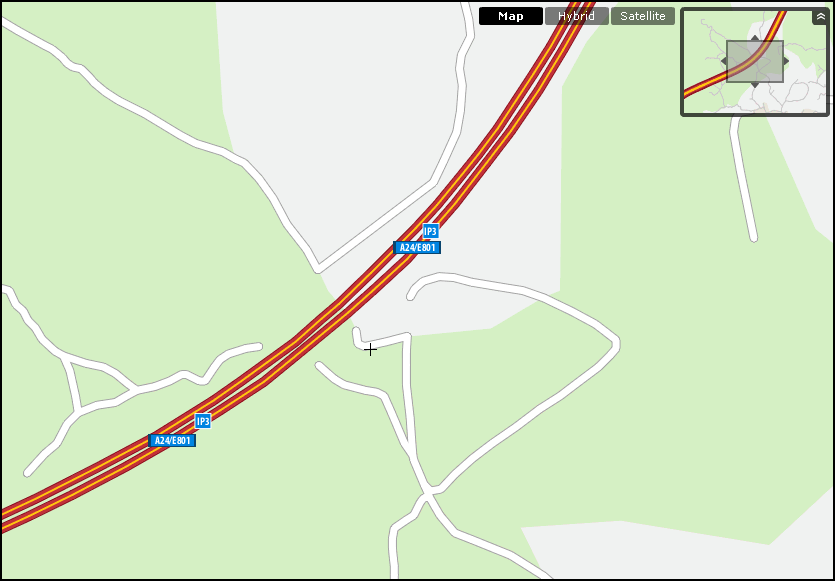
\includegraphics[width=.6\mycolumnwidth]{Fundamentos_cartograficos/Generalizacion_agregacion.png}
\caption{\small Un ejemplo de generalizaci�n por agregaci�n. Dos carreteras pr�cticamente paralelas y unidas se representan como dos elementos en el mapa, pero en el localizador de la parte superior izquierda, a escala de menor detalle, se generalizan como una �nica (Tomado de Yahoo Maps).}
\label{Fig:Generalizacion_agregacion} 
\end{figure}

Combinando operaciones como las anteriores de forma adecuada, se obtiene una cartograf�a mucho m�s �til, en la cual la informaci�n que contiene resulta m�s accesible y pr�ctica, con un mayor potencial desde todos los puntos de vista. En el caso de trabajar en un SIG, algunas de estas operaciones, como pueden ser la simplificaci�n o la agregaci�n, tiene tambi�n un efecto beneficioso sobre el propio manejo de los datos dentro del SIG.

Estas operaciones se enumeran aqu� como ideas a aplicar para efectuar la generalizaci�n de un documento geogr�fico, como corresponde a este cap�tulo de fundamentos y conceptos cartogr�ficos b�sicos. No obstante, estas mismas operaciones tambi�n las veremos en otras partes del libro, ya que no son exclusivas de esta parte. Por su importante papel en la representaci�n visual de los datos, veremos m�s al respecto en la parte dedicada a visualizaci�n. Algunos algoritmos para la simplificaci�n y suavizado de l�neas\index{Suavizado!de l�neas} los estudiaremos en la parte dedicada a procesos, particularmente en el apartado \ref{Generalizacion_lineas}.

\subsection{Generalizaci�n en el contexto de un SIG}\label{Generalizacion_en_SIG}

La generalizaci�n es importante en un SIG debido a la variedad de escalas posibles que puede tener la informaci�n con que se trabaja, as� como por la variedad de escalas de representaci�n que pueden definirse gracias a la flexibilidad que el propio SIG presenta en sus capacidades de visualizaci�n. Existen diversas formas de enfocar inicialmente el problema de obtener un juego de datos �ptimo para ser representado en cada caso y una representaci�n �ptima de este.

La mayor problem�tica se encuentra en el manejo de datos con gran precisi�n y gran volumen ---como, por ejemplo, esos datos de calles y v�as de todo el mundo--- al representarlos a una escala de menor detalle, aunque el proceso de generalizaci�n no es necesario exclusivamente en este caso, sino en muchos otros con independencia del volumen y la escala original. 

Una aproximaci�n b�sica puede ser trabajar con todo el conjunto de datos y generalizarlo a medida que sea necesario en funci�n de la escala de trabajo en cada momento. Es decir, si el usuario decide visualizar todo un continente, el SIG no traza todas las calles de ese continente, sino que se seleccionan de forma autom�tica los objetos a ser visualizados y despu�s se crea la representaci�n. Las operaciones de generalizaci�n se llevan a cabo en el momento mismo en que el usuario lo necesita.

Este tipo de generalizaci�n <<al vuelo>>\index{Generalizaci�n!cartogr�fica!al vuelo} no resulta, sin embargo, �ptimo, y en la mayor�a de los casos es inviable o no proporciona los resultados esperados. Esto es as� debido a que se ha de trabajar con el gran volumen de datos original, y generalizar estos es una tarea suficientemente compleja como para que los algoritmos encargados de hacerlo no lo hagan de forma fluida. No ha de olvidarse que, mientras que la raz�n fundamental de la generalizaci�n en el contexto de la cartograf�a cl�sica es la mera visualizaci�n y la transmisi�n de la informaci�n, en el entorno de un SIG tambi�n existen razones relacionadas con la eficiencia de los procesos, como ya se ha mencionado. Aplicando esta metodolog�a, la generalizaci�n no es ventajosa en t�rminos de c�mputo, sino que, por el contrario, puede incluso suponer una carga adicional al proceso de visualizaci�n.

Aun en el caso de que el volumen de datos no fuera grande y no existieran problemas de rendimiento, una generalizaci�n por completo automatizada no garantiza un resultado �ptimo. Aun existiendo algoritmos y formulaciones matem�ticas que permiten generalizar de forma relativamente adecuada (algunos de los cuales los veremos m�s adelante en este libro), el proceso global de generalizaci�n combina varios procedimientos distintos, y en conjunto conforma un proceso no exento de subjetividad. La labor tradicional del cart�grafo no puede automatizarse de forma total, y se hace necesario cierto trabajo manual para obtener un resultado de calidad o evaluar el generado por un procedimiento autom�tico.

Por todo lo anterior, la forma de incorporar la generalizaci�n dentro de un SIG suele basarse en un enfoque multi--escalar, en el cual se maneja informaci�n de una misma zona de estudio a diferentes escalas, y se usa en cada momento aquella que resulte m�s conveniente. Si trabajara con cartograf�a en papel, ser�a equivalente a tener varios mapas de una zona a diferentes escalas.

Por ejemplo, en un mapa con n�cleos de poblaci�n a escala 1:25000\index{Escala} se almacenar� cada ciudad como un pol�gono que delimite su contorno. Esa misma informaci�n a escala 1:1000000 se almacenar� como un �nico punto cada ciudad, ya que el tama�o de esta es demasiado peque�o en la representaci�n, y no tiene sentido el empleo de tanto detalle. Para convertir un mapa en otro se ha producido un proceso de simplificaci�n, convirtiendo pol�gonos en puntos.

Si incorporamos ambos mapas dentro de un SIG, podemos utilizar el que corresponda en funci�n de la escala requerida. De este modo, la generalizaci�n no es una tarea que el propio SIG desarrolle, sino que cuando esta es necesaria puede recurrir a una informaci�n ya generalizada de antemano. El rendimiento del proceso es mayor, y adem�s el dato generalizado puede haber sido elaborado de la forma m�s conveniente.

El concepto de \emph{capa},\index{Capa} que veremos en el cap�tulo \ref{Introduccion_datos} y que es vital para la idea actual de un SIG, permite este manejo simult�neo de informaci�n a distintas escalas.

En la figura \ref{Fig:SIG_multi_escala} puede verse un esquema de lo anterior. A medida que variamos la escala de representaci�n, la informaci�n que vemos representada tiene una escala distinta y podr�a tambi�n tener un distinto origen. Incluso el tipo de informaci�n que vemos var�a, ya que las representaciones m�s globales son de tipo gr�fico, creadas a partir de los propios datos almacenados como objetos (calles, carreteras, etc.), mientras que la de mayor detalle es una fotograf�a a�rea.


\begin{figure}
\centering
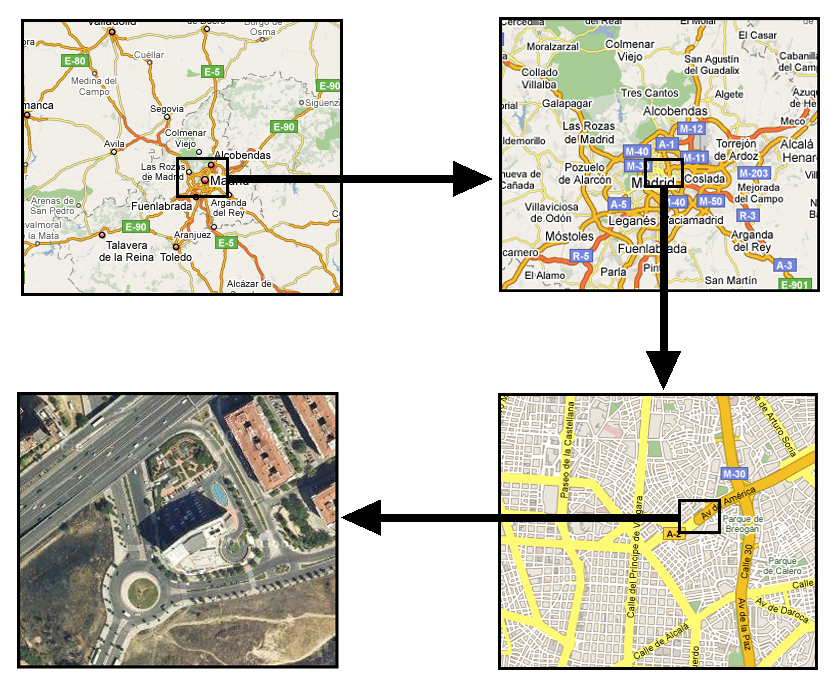
\includegraphics[width=.9\textwidth]{Fundamentos_cartograficos/SIG_multi_escala.png}
\caption{\small En un SIG es habitual manejar informaci�n a diferentes escalas. En funci�n de la escala de representaci�n, la informaci�n visualizada ser� una u otra.}
\label{Fig:SIG_multi_escala} 
\end{figure}

En el caso de im�genes tales como esa fotograf�a a�rea, existen adem�s en un SIG una serie de procesos que tambi�n pueden considerarse como parte de la generalizaci�n, y que ata�en m�s al rendimiento que a la representaci�n. Para entenderse esto pi�nsese que las im�genes se componen de elementos denominados \extr{p�xeles}, que son peque�os puntos, cada uno de los cuales tendr� un color asociado (esto lo veremos con mucho m�s detalle en el cap�tulo \ref{Tipos_datos}). El numero de estos p�xeles en una imagen grande es muy superior al de una pantalla (una pantalla tambi�n se divide en puntos, si te acercas a una lo podr�s ver claramente). 

El proceso de representaci�n de la imagen en la pantalla consiste en calcular qu� color asignar a cada p�xel de la pantalla en funci�n de los de la imagen, pero este proceso, si se utiliza la imagen completa, es muy costoso en t�rminos de c�mputo, ya que implica procesar toda la informaci�n de la imagen, que puede ser del orden de centenares de millones de p�xeles. Si representamos una porci�n de esa imagen (una porci�n del territorio que cubre), podemos solo trabajar con los p�xeles en esa zona, pero la representaci�n de toda la imagen hace necesario procesar todos los valores que contiene.\index{Pixel}

Este proceso en realidad puede verse como un tipo de generalizaci�n <<al vuelo>>. Ya dijimos que este ten�a principalmente dos problemas: el rendimiento y la imposibilidad de obtener resultados �ptimos de forma automatizada. En el caso de im�genes, existe el problema del rendimiento, pero es posible automatizar la creaci�n de datos a diferente escala de trabajo. Esto es as� debido a que la representaci�n de elementos tales como carreteras o lagos se hace mediante una interpretaci�n de esos objetos, y este proceso es en cierta medida subjetivo, como vimos.  En el caso de im�genes no hay que interpretar objeto alguno, ya que esos objetos ya <<est�n>> representados en la imagen, y �nicamente es necesario disminuir la escala.

\begin{figure}
\centering
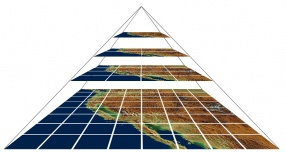
\includegraphics[width=.45\textwidth]{Fundamentos_cartograficos/Piramide.png}
\caption{\small Pir�mides de representaci�n con im�genes preparadas a distintas escalas (Fuente: OSGeo).}
\label{Fig:Piramides} 
\end{figure}

Los algoritmos para llevar a cabo este proceso se conocen como de \emph{remuestreo}\index{Remuestreo}, y los veremos con detalle en el cap�tulo \ref{Algebra_de_mapas}. Algunos SIG utilizan estos algoritmos para hacer m�s fluido el manejo de grandes im�genes mediante la creaci�n de las denominadas \emph{pir�mides}. Cuando el usuario introduce en el SIG una imagen de gran tama�o, este prepara varias versiones de esa imagen a distintas escalas de detalle, de forma que posteriormente pueda recurrir a la que sea m�s conveniente en cada caso en funci�n de la escala de representaci�n. Es decir, el SIG realiza la <<generalizaci�n>> de esa imagen de forma autom�tica, siendo necesario proporcionarle �nicamente la imagen de mayor detalle. La figura \ref{Fig:Piramides} ilustra gr�ficamente esto. \index{Pir�mides}


\section{Resumen}

La cartograf�a y la geodesia son ciencias que aportan un importante conjunto de conocimientos y elementos al mundo de los SIG, y su estudio es fundamental para cualquier trabajo con un SIG.

La geodesia se encarga de estudiar la forma de la Tierra, con objeto de posteriormente poder localizar de forma precisa los puntos sobre esta mediante un sistema de coordenadas. Dos conceptos b�sicos en geodesia son el \emph{geoide} y el \emph{elipsoide}, superficies de referencia que modelizan la forma de la Tierra. El primero es la superficie formada por los puntos en los que el campo gravitatorio tiene una misma intensidad, y se obtiene prolongando la superficie de los oc�anos en reposo bajo la superficie terrestre. El segundo es un objeto definido por una ecuaci�n y una serie de par�metros, que permite asimilar la Tierra a una superficie matem�tica.

El conjunto de un elipsoide y un punto de tangencia con la superficie terrestre (Punto Fundamental), forma un \emph{datum}.

Para asignar coordenadas a un punto en funci�n de los elementos anteriores es necesario definir un sistema de referencia. Las coordenadas geogr�ficas han sido utilizadas tradicionalmente, y son de utilidad para grandes zonas. Otro tipo de coordenadas m�s intuitivas son las cartesianas, y para su obtenci�n se requiere el concurso de una proyecci�n cartogr�fica que convierta coordenadas espaciales en coordenadas planas. Hay muchos tipos de proyecciones, siendo el sistema UTM uno de los m�s extendidos.

En el �mbito de la cartograf�a, hemos visto en este cap�tulo la importancia del concepto de escala, que no pierde su papel fundamental al trabajar en un SIG en lugar de hacerlo con cartograf�a impresa. Estrechamente relacionada con la escala encontramos la \emph{generalizaci�n}, que comprende una serie de procesos encaminados a la obtenci�n de una representaci�n lo m�s clara posible de una serie de datos a una escala dada.

%\bibliographystyle{unsrt}
%\bibliography{../../Libro_SIG}

